\chapter{On the production of entangled beams from a metastable helium BEC}
\label{Peaks}
\graphicspath{{Figures/Peaks/}{Figures/Common/}}

In this chapter we investigate the production of paired atom laser beams from a metastable helium condensate due to an unusual scattering process.  Radio-frequency outcoupling is used to extract atoms from a Bose-Einstein condensate to initiate scattering between trapped and untrapped atoms.  The unequal strengths of the interactions for different internal states allows an energy-momentum resonance which leads to the scattering of atoms from the zero-velocity condensate into modes of opposite momenta.  This process is shown to be the result of dynamical instabilities within the condensate that originate from a process analogous to optical parametric down-conversion, giving rise to entanglement between the unstable modes.  These unstable modes are outcoupled to form scattered beams well-separated from the main atom laser profile, which are observed experimentally.

The results presented in \sectionref{Peaks:PerturbativeApproach} of this chapter are in preparation for submission, while the results presented in \sectionref{Peaks:3DCalculation} of this chapter have been published in~\citet{Dall:2009}.  All of the theoretical work in these papers was my own work with the exception of the classical propagation discussed at the end of \sectionref{Peaks:AbsorbingBoundaryTricks}.

\section{Introduction}
Sources of matter waves gained a dramatic improvement with the achievement of Bose-Einstein condensation (BEC) in dilute gases and the development of the atom laser~\citep{Anderson:1995vn,Mewes:1997}. Like optical lasers before them, atom lasers can produce Heisenberg-limited beam profiles~\citep{Busch:2002zr,Riou:2006uq} and promise high spectral density through their dramatically lower linewidth~\citep{Wiseman:1997ba}. Another exciting possibility resulting from having such a coherent source of atoms is the generation of nonclassical matter waves such as entangled beams. Entangled beams are useful for tests of quantum mechanics and are required to perform Heisenberg-limited interferometry~\citep{Dowling:1998,Reid:1988}.  In this chapter, we show that the asymmetric scattering lengths between internal states of metastable helium (He*) cause well-defined peaks in the output of an atom laser.  These peaks are due to a dynamical instability in the condensate that originates from a process that generates entanglement.

A nonlinear process is required to produce entanglement, and one of the advantages of atomic systems over optical systems is that there are strong inherent nonlinearities due to atomic interactions, although these interactions can also lead to complications. These nonlinearities allow certain analogues of nonlinear optical experiments such as four-wave mixing, parametric down-conversion and Kerr squeezing to be performed directly in the atomic sample~\citep{WallsMilburn}. All of these produce non-classical states in optical systems. Four-wave mixing in a trapped BEC has been demonstrated experimentally in configurations where three distinct momentum states generated a fourth~\citep{Deng:1999qy} and where two momentum states generated a pair of correlated atomic beams~\citep{Vogels:2002}. These experiments demonstrated that the output phase was coherent, but the correlation properties were not measured. More recently the pair correlations in a spontaneous scattering of two colliding condensates were measured using the single-atom detectors available for He* atoms~\citep{Perrin:2007}.

Using these existing sources of entangled pairs of atoms for interferometric experiments will be complicated by the high densities of the sources, where the nonlinearities that generated the correlations ultimately degrade the long-term coherence of the sample. While recent experiments have increased the coherence of atom interferometers by several orders of magnitude by reducing the nonlinearities with a Feschbach resonance~\citep{Fattori:2008,Gustavsson:2008}, this precludes the production of entangled pairs.  In the scheme presented here the nonlinear interactions are used to drive dynamical instabilities in the condensate, but the resulting untrapped beams that propagate in free space are dilute, potentially avoiding the decoherence problem.  We show that pairs of beams can be produced simply by the process of radio-frequency (rf) outcoupling from a He* BEC, without the need for Feschbach resonances or scattering pulses.  Unlike previous methods, which required pairs of atoms travelling at high kinetic energies as a source, this process involves scattering between atoms initially in the same zero-momentum state to create states with nonzero momentum.  Semiclassical and field-theoretic simulations of the experiment show that the beams are generated by the same parametric down-conversion process that generates entangled optical beams.  Although the beams in the present experiment will not retain all of the original non-classical correlations produced by the dynamical instabilities, some will remain and a future experiment is proposed that may enable the full correlations produced by the dynamical instabilities to be extracted from the condensate.

\section{The metastable helium `Peaks' experiment}
\label{Peaks:ExperimentalSetup}

The experimental setup for creating He* BEC has been reported elsewhere~\citep{Dall:2007a}. The experiment discussed in this section was performed by \emph{Robert Dall}, \emph{Lesa Byron} and \emph{Andrew Truscott} at the Research School of Physics and Engineering, ANU.

Starting from an almost pure BEC containing up to $2\times 10^6$ atoms, an atom laser beam was created by using rf photons to spin flip the BEC atoms from the $m_F=1$ magnetically trapped state to the $m_F=0$ untrapped state.  After outcoupling, atoms in the atom laser beam fell under gravity for a distance of $\unit[4]{cm}$ until they hit a double-stacked multichannel plate (MCP). The phosphor screen was imaged with a charge-coupled-device (CCD) camera with a resolution of approximately $\unit[150]{\micro m}$ at the MCP. To remove any nonuniformities caused by spatial variations in the gain of the MCP, all images were divided by a flat-field image produced by dropping atoms from a MOT onto the detector. Since the MOT temperature is of order $\sim\unit[1]{mK}$, the spatial profile of the MOT uniformly illuminates the MCP. Although $m_F=-1$ atoms are produced by the outcoupling, especially for high rf powers, they are in general accelerated away from the detector by the magnetic trap field. Those that are accelerated towards the detector do not show up in the images since they arrive much earlier than the CCD trigger time.

\figureref{Peaks:ExperimentalResults} shows the dramatic change in the atom laser spatial profile when the dynamical instabilities in the condensate are excited.  In the case of low outcoupling Rabi frequencies (upper row), this process does not occur and we see the usual double-peaked He*-atom laser profile~\citep{Dall:2007} (see also \sectionref{BackgroundTheory:TransverseProfile}). When the Rabi frequencies are high enough to drive the instabilities (lower row), the atoms in the atom laser beam are scattered to form a halo around the main atom laser beam.  Due to conservation of energy, the outer diameter of this halo corresponds to a maximum kinetic energy given by the chemical potential.  As well as the ring structure, four peaks are observed on the outskirts of the profile.
% Each peak contains 11\%--14\% of the total outcoupled atoms, in agreement with the value of 11\% obtained from the simulation results shown in the lower row of \figureref{Peaks:ExperimentalResults}.

These peaks arise from two momentum-correlated cones of particles scattering out of the condensate and falling to the detector, as shown in \figureref{Peaks:Schematic}.  The cones themselves are generated by a dynamical instability that populates momentum modes lying along the weak trapping axis, which expand to rings due to the mean-field repulsion in the tight trapping direction as they leave the BEC.  Atoms in these cones then fall under gravity onto the detector, where the time-integrated flux is converted to a spatial density distribution, and each momentum ring appears as a double peak.  The background halo is produced during the initial switch-on of the atom laser during which the peaks produced by the instabilities sweep in position from the main atom laser profile towards their final position in \figureref{Peaks:ExperimentalResults}.

A summary of the relevant parameters of the experiment is given in \tableref{Peaks:ExperimentalParameters}.

\begin{figure}
    \centering
        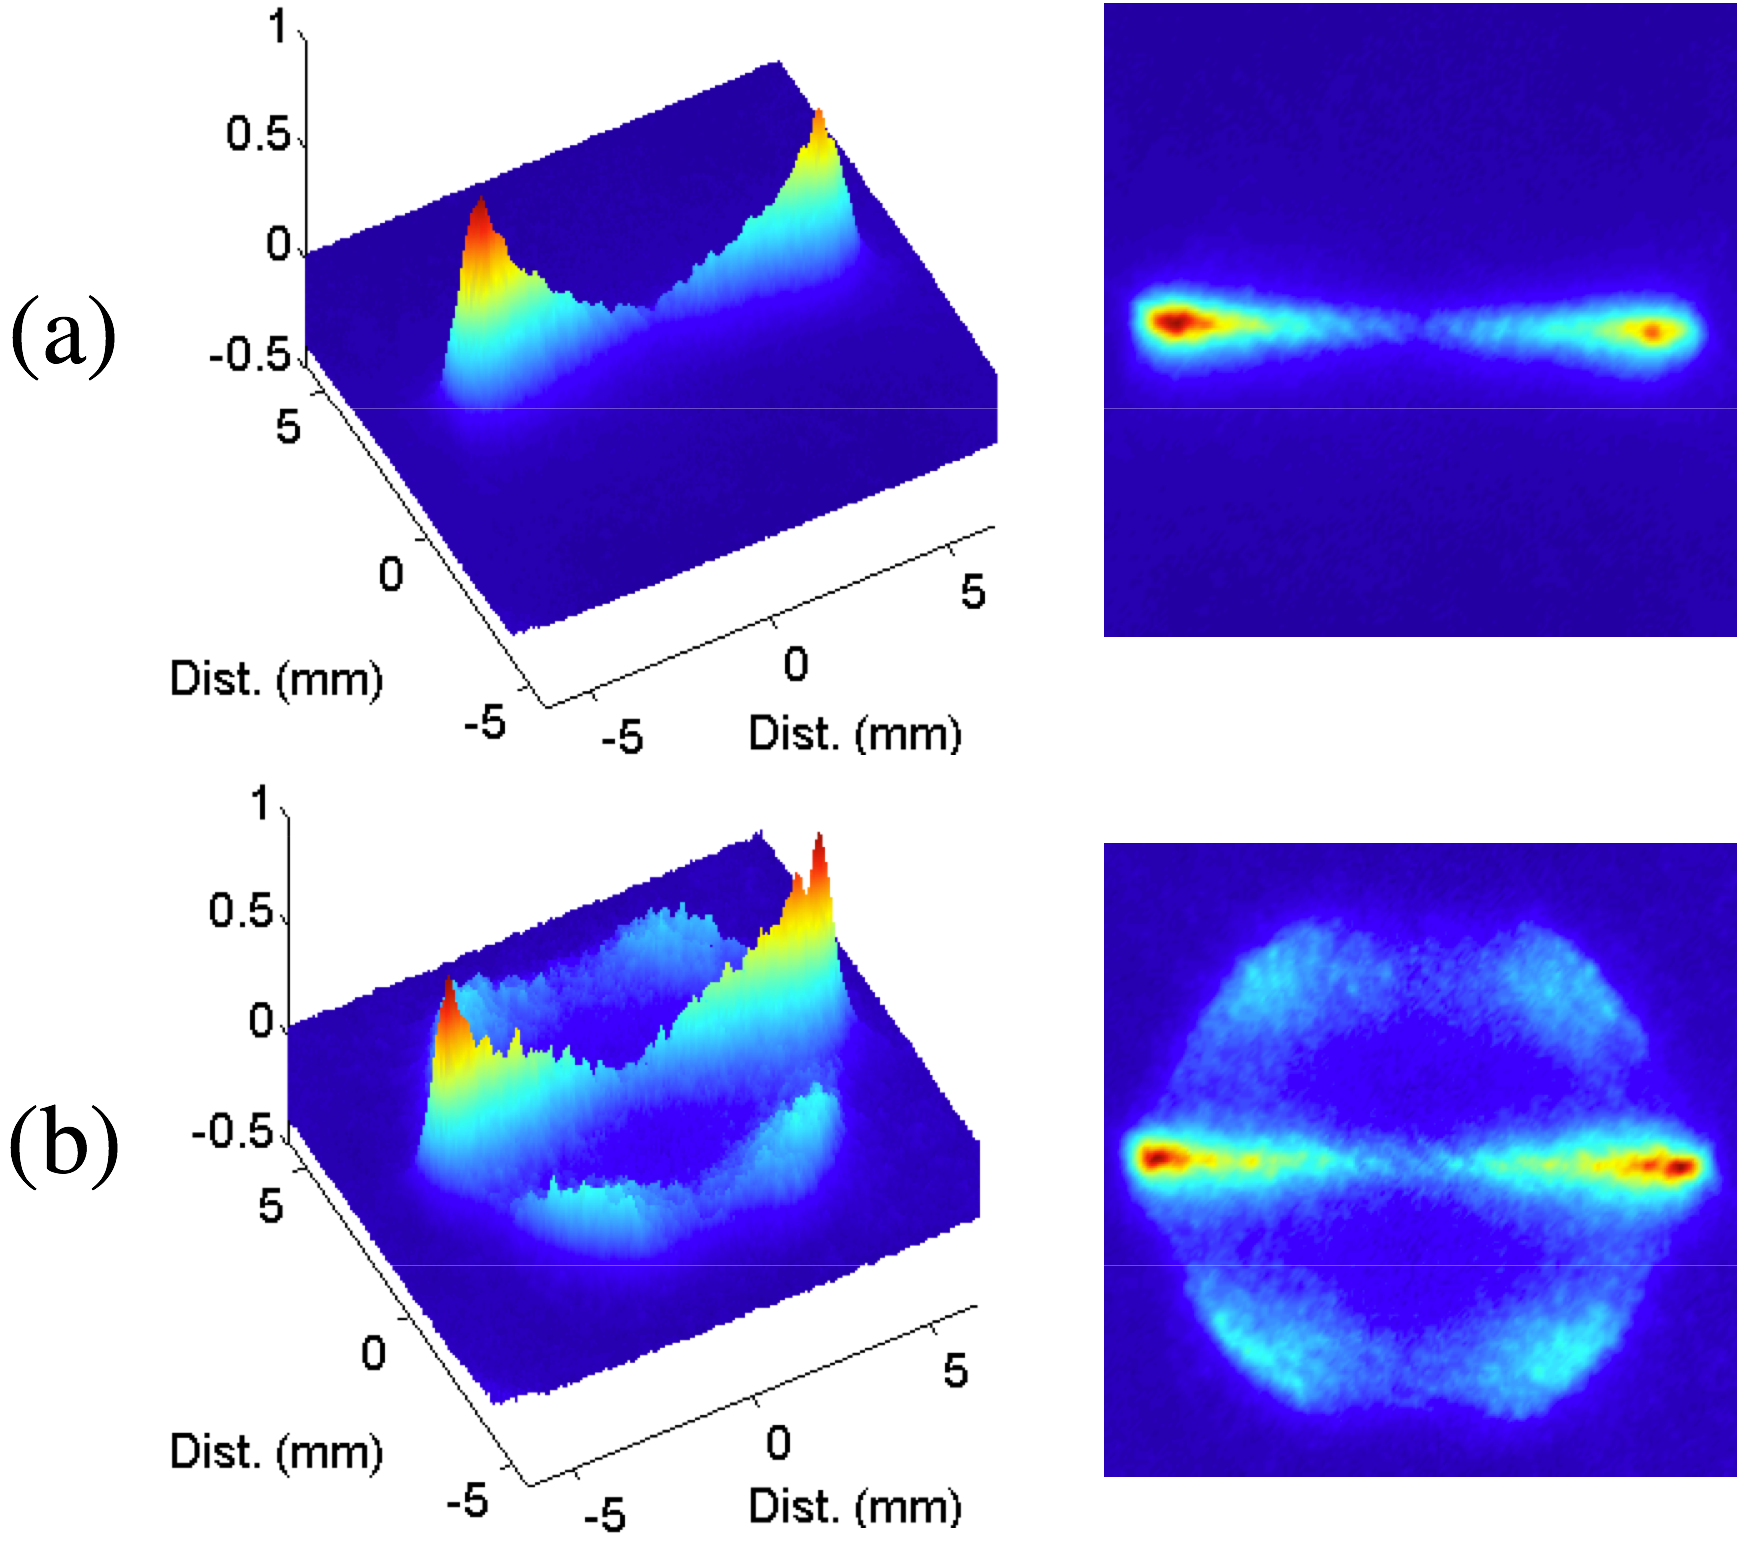
\includegraphics[height=3in]{ExperimentalResults}
    \caption{Experimental results. The difference between (a) and (b) is that the outcoupling Rabi frequency has been increased by an order of magnitude in (b).}
    \label{Peaks:ExperimentalResults}
\end{figure}

\begin{figure}
    \centering
        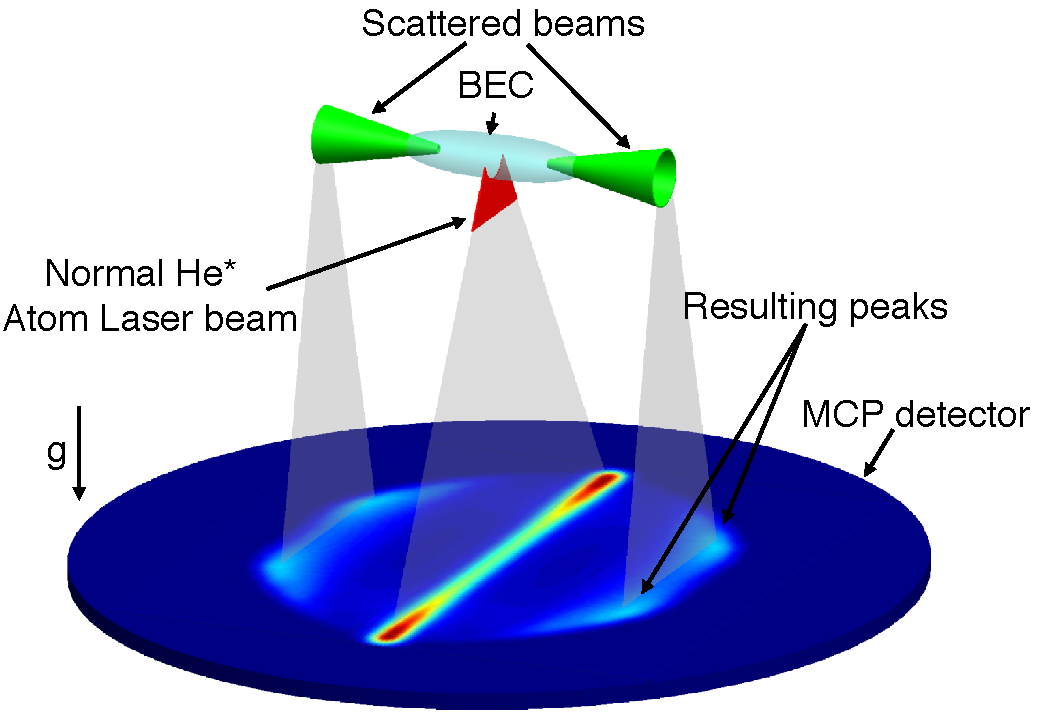
\includegraphics[height=3in]{Schematic}
    \caption{Schematic of the experimental setup}
    \label{Peaks:Schematic}
\end{figure}


\begin{table}
    \centering
    \begin{tabular}{ccc}
    \toprule
    Parameter & Value\\
    \midrule
    Condensate number & $N = 2\times 10^6$\\
    Radial trapping frequency & $\omega_r = 2 \pi \times \unit[1020]{Hz}$\\
    Axial trapping frequency & $\omega_z = 2\pi \times \unit[55]{Hz}$\\
    Outcoupling Rabi frequency & $\Omega = 2\pi \times \unit[6.5]{kHz}$\\
    Quasimolecule $S=0$ scattering length & $a_{S=0}=\unit[9.46]{nm}$\\
    Quasimolecule $S=2$ scattering length & $a_{S=2}=\unit[7.51]{nm}$\\
    Penning ionisation rate  & $\Kunpol = \unit[7.7\times 10^{-17}]{m\textsuperscript{3}}$ & \citep{Stas:2006kx}\\
    \bottomrule
    \end{tabular}
    \caption{Experimental parameters for the metastable helium BEC under consideration.  FIXME: Review this table.}
    \label{Peaks:ExperimentalParameters}
\end{table}

\section{Overview of Bogoliubov theory}
\label{Peaks:ElementaryExcitations}

The observed features in the atom laser profile presented in the previous section are caused by a dynamical instability in the condensate. The modes that are dynamically unstable are identified in the next section, in which the excitation spectrum of the condensate is obtained. In this section an overview is given of the Bogoliubov theory which is used to obtain the excitation spectrum of the condensate and to determine its stability. More comprehensive treatments of the Bogoliubov theory are given in~\citep{PethickSmith} and in a number of review articles~\citep{Leggett:2001,Ozeri:2005,Proukakis:2008}.

The problem is to determine the response of the condensate to small fluctuations about the mean-field. Typically the condensate is stable to such fluctuations, and their energy spectrum determines the phase and group velocities of the excitations.  In the case that the condensate is dynamically unstable some modes will undergo exponential growth, which corresponds to the generalised energy spectrum containing nonzero imaginary components. As a concrete example of the techniques demonstrated in this section, we consider a single-component condensate described by the Hamiltonian
\begin{align}
    \label{Peaks:ElementaryExcitationsExampleHamiltonian}
    \hat{H} &= \int d \vect{x}\, \hat{\Psi}^\dagger \left( -\frac{\hbar^2 \nabla^2}{2 M} + V(\vect{x}) + \frac{1}{2} U \hat{\Psi}^\dagger \hat{\Psi} - \mu \right) \hat{\Psi},
\end{align}
where an arbitrary energy offset $\mu$ has been included. This term is introduced for calculational reasons and has no physical influence on the Hamiltonian\footnote{The energy offset cannot affect any observable expectation values as although it contributes a different energy offset for states with different total number, these states are uncoupled due to the conservation of particle-number.}.

The principal idea in finding the excitation spectrum of \eqref{Peaks:ElementaryExcitationsExampleHamiltonian} is to take advantage of the usefulness of the Gross-Pitaevskii equation in describing the mean-field of the condensate to enable the quantum-mechanical fluctuations about the mean-field to be considered. To this end the deviation operator $\delta \hat{\Psi} = \hat{\Psi} - \Psi$ is defined, where $\Psi = \mean{\hat{\Psi}}$, and $\delta \hat{\Psi}$ is considered to be a small quantity\footnote{For $\delta\hat{\Psi}$ to be considered a small quantity, the mean field $\mean{\hat{\Psi}}$ must be non-zero. However the state of condensates with a large number of atoms is well approximated by either a state with well-defined total number or as a mixture over global phase of coherent states (see \sectionref{BackgroundTheory:GrossPitaevskiiEquation}), for both of these the mean field $\mean{\hat{\Psi}}$ is zero. Despite this, as any \emph{physical} expectation value is independent of the choice of global phase, the analysis presented here can be performed for a coherent state with a given global phase and the results then averaged over that global phase. As all physical expectation values are independent of the global phase this averaging step cannot change the results and can be omitted.}. The Hamiltonian \eqref{Peaks:ElementaryExcitationsExampleHamiltonian} can then be expanded in powers of $\delta \hat{\Psi}$,
\begin{align}
    \label{Peaks:HamiltonianPowerSeriesExpansion}
    \hat{H} &= \hat{H}_0 + \hat{H}_1 + \hat{H}_2 + \hat{H}_3 + \hat{H}_4,
\end{align}
where $\hat{H}_n$ contains terms of order $(\delta\hat{\Psi})^n$. The excitation spectrum of the Hamiltonian $\hat{H}$ is then approximately given by the eigenvalue spectrum of the lowest order non-trivial term in \eqref{Peaks:HamiltonianPowerSeriesExpansion}.

The zeroth order term in \eqref{Peaks:HamiltonianPowerSeriesExpansion}
\begin{align}
    \hat{H}_0 &= \int d \vect{x}\, \Psi^* \left( -\frac{\hbar^2 \nabla^2}{2M} + V(\vect{x}) + \frac{1}{2} U \big|\Psi\big|^2 - \mu \right) \Psi
\end{align}
is simply a constant and represents the total energy of the unexcited mean-field. The first order term is of the form
\begin{align}
    \hat{H}_1 &= \int d \vect{x}\, \delta \hat{\Psi}^\dagger \left(i \hbar \frac{\partial \Psi}{\partial t} \right)  + \int d \vect{x}\, \left(i \hbar \frac{\partial \Psi}{\partial t} \right)^* \delta \hat{\Psi},
\end{align}
where the mean-field $\Psi$ evolves as
\begin{align}
    i \hbar \frac{\partial\Psi}{\partial t} &= \left(-\frac{\hbar^2 \nabla^2}{2 M} + V(\vect{x}) + U \big| \Psi\big|^2 - \mu \right) \Psi.
\end{align}

Although the first order term $\hat{H}_1$ is nonzero, it does not affect the evolution of the deviation operator:
\begin{align}
    i \hbar \frac{\partial }{\partial t}\hat{\Psi} &= \comm{\hat{\Psi}, \hat{H}}\\
    i \hbar \frac{\partial }{\partial t}\delta{\hat{\Psi}} + i \hbar \frac{\partial \Psi}{\partial t} &= \comm{\Psi, \hat{H}} + \comm{\delta\hat{\Psi}, \hat{H}}\\
    i \hbar \frac{\partial }{\partial t}\delta \hat{\Psi} &= \comm{\delta \hat{\Psi}, \hat{H}} - i \hbar \frac{\partial  \Psi}{\partial t}\\
    &= \comm{\delta \hat{\Psi}, \hat{H}_1} + \comm{\delta \hat{\Psi}, \hat{H}_2 + \hat{H}_3 + \hat{H}_4} - i \hbar \frac{\partial\Psi }{\partial t}\\
    &= i \hbar \frac{\partial \Psi}{\partial t} + \comm{\delta \hat{\Psi}, \hat{H}_2 + \hat{H}_3 + \hat{H}_4} - i \hbar \frac{\partial \Psi}{\partial t}\\
    &= \comm{\delta \hat{\Psi}, \hat{H}_2 + \hat{H}_3 + \hat{H}_4}. \label{Peaks:DeviationOperatorEvolution}
\end{align}
As $\hat{H}_1$ does not occur in \eqref{Peaks:DeviationOperatorEvolution}, it does not affect the evolution of the deviation operators and so will not contribute to the excitation spectrum\footnote{Typical treatments of the Bogoliubov theory consider the restricted case of a static condensate density and choose $\mu$ as the chemical potential such that $\displaystyle \frac{\partial \Psi}{\partial t} = 0$, and hence $\hat{H}_1=0$. As shown by \eqref{Peaks:DeviationOperatorEvolution}, this choice of $\mu$ is unnecessary as $\hat{H}_1$ does not influence the evolution of $\delta\hat{\Psi}$, \emph{independent} of the choice of $\mu$ and even in the general case of a non-stationary mean field. This latter case is considered in \sectionref{Peaks:PerturbativeApproach}.}.

The first physically important term in \eqref{Peaks:HamiltonianPowerSeriesExpansion} is
\begin{align}
    \begin{split}
        \hat{H}_2 &= \int d \vect{x}\, \delta \hat{\Psi}^\dagger \left(-\frac{\hbar^2 \nabla^2}{2 M} + V(\vect{x}) + 2 U\big|\Psi\big|^2 -\mu \right)\delta\hat{\Psi}\\
         &\relphantom{=} + \frac{1}{2} U\int d \vect{x}\, \left(\Psi^2 \delta \hat{\Psi}^\dagger\delta \hat{\Psi}^\dagger  +  (\Psi^*)^2 \delta \hat{\Psi} \,\delta \hat{\Psi}\right).
    \end{split}
    \label{Peaks:HamiltonianPowerSeriesQuadraticTerm}
\end{align}
As the deviation operator $\delta \hat{\Psi}$ is small compared to the mean field $\Psi$, the higher-order contributions $\hat{H}_3$ and $\hat{H}_4$ to the total Hamiltonian can be neglected compared to $\hat{H}_2$. The excitation spectrum of the condensate about the mean field $\Psi$ is then given by the energy spectrum of $\hat{H}_2$.

To avoid directly solving the infinite dimensional eigenvalue problem $\hat{H}_2 \ket{\Psi} = E \ket{\Psi}$ for the condensate excitation spectrum, it is desired to apply a linear transformation to $\hat{H}_2$ that will diagonalise it in the form
\begin{align}
    \label{Peaks:QuadraticHamiltonianAnsatz}
    \hat{H}_2 &= \sum_i \hbar \omega_i \hat{\Lambda}_i^\dagger \hat{\Lambda}_i^{\phantom{\dagger}},
\end{align}
for some boson annihilation operators $\hat{\Lambda}_i$ and real frequencies $\omega_i$. In this form, the Hamiltonian can be simply interpreted as representing a set of modes with energies $\hbar \omega_i$, which is the condensate excitation spectrum. The eigenvalues of $\hat{H}_2$ can also be identified as $\{n \hbar \omega_i : n > 0 \}$. It is not possible in general to transform $\hat{H}_2$ into the form \eqref{Peaks:QuadraticHamiltonianAnsatz} if the Hamiltonian possesses any instabilities~\citep{Leonhardt:2003}, however one frequently considers the excitation spectrum of the ground state which is stable by definition and in this case such a transformation is always possible.

In the general case, we look for the operators $\hat{\Lambda}_i$ satisfying
\begin{align}
    \label{Peaks:ElementaryExcitationsEvolution}
    i \hbar \frac{\partial }{\partial t}\hat{\Lambda}_i &= \comm{\hat{\Lambda}_i, \hat{H}_2 } = - \hbar \omega_i \hat{\Lambda}_i
\end{align}
where $\omega_i$ is real if and only if $\hat{\Lambda}_i$ is a boson annihilation operator~\citep{Leonhardt:2003}. In the case that $\omega_i$ is complex, boson annihilation operators can be constructed from the $\hat{\Lambda}_i$ as discussed in \appendixref{FloquetAppendix}. Hence $\hbar\omega_i$ can be considered to be a generalised energy spectrum of the condensate where nonzero imaginary components correspond to dynamical instabilities of the condensate. Note that although the eigenvalues of $\hat{H}_2$ must be real as it is Hermitian, the eigenvalues of \eqref{Peaks:ElementaryExcitationsEvolution} need not be real. For example, the Hamiltonian for degenerate parametric down-conversion $\hat{H} = \hbar\chi \left(\hat{a}\hat{a} + \hat{a}^\dagger \hat{a}^\dagger \right)$ is Hermitian but the corresponding eigenvalues of \eqref{Peaks:ElementaryExcitationsEvolution} are pure imaginary. In this case the occupation of the mode $\hat{a}$ undergoes exponential growth. The case of complex eigenvalues $\omega_i$ is discussed further in \sectionref{Peaks:ExperimentEigenvalues} and \appendixref{FloquetAppendix}.

Equation \eqref{Peaks:ElementaryExcitationsEvolution} is most easily solved by expanding the $\hat{\Lambda}_i$ in a complete, linearly independent basis $\{\hat{\Upsilon}_j\}$ such that $\hat{\Lambda}_i = \vect{c}_i^\dagger \hat{\vect{\Upsilon}}$ where $\vect{c}_i$ is a complex vector, $\vect{c}_i^\dagger$ denotes the conjugate-transpose, and $\hat{\vect{\Upsilon}}$ is the column vector formed by the complete basis $\{\hat{\Upsilon}_j\}$. For the case of \eqref{Peaks:HamiltonianPowerSeriesQuadraticTerm}, an appropriate basis is $\{\hat{\Upsilon}_j\} = \{\delta\hat{\Psi}, \delta\hat{\Psi}^\dagger\}$. As the Hamiltonian $\hat{H}_2$ is quadratic, its commutator with every operator $\hat{\Upsilon}_j$ will be linear in the operators $\{\hat{\Upsilon}_j\}$. Defining the complex matrix $\mathcal{H}$ to represent this relationship
\begin{align}
    \label{Peaks:ScriptHRelationshipToHamiltonian}
    \sum_k \mathcal{H}_{jk} \hat{\Upsilon}_k &= \comm{\hat{\Upsilon}_j, \hat{H}_2}
\end{align}
permits \eqref{Peaks:ElementaryExcitationsEvolution} to be recast as an eigenvalue problem in $\mathcal{H}$,
\begin{align}
    \comm{\vect{c}_i^\dagger \hat{\vect{\Upsilon}}, \hat{H}_2} &= \vect{c}_i^\dagger \mathcal{H} \hat{\vect{\Upsilon}} = - \hbar \omega_i \vect{c}_i^\dagger \hat{\vect{\Upsilon}}, \label{Peaks:ElementaryExcitationsEigenvalueProblemWithOperators}\\
    \implies \vect{c}_i^\dagger \mathcal{H} &= - \hbar \omega_i \vect{c}_i^\dagger \label{Peaks:ElementaryExcitationsEigenvalueProblem}
\end{align}
where the last line follows as the components of $\hat{\vect{\Upsilon}}$ are linearly independent. If the mean-field $\Psi$ is time-independent, then the matrix $\mathcal{H}$ will also be time-independent and \eqref{Peaks:ElementaryExcitationsEigenvalueProblem} represents an eigenvalue problem for the left eigenvectors $\vect{c}_i^\dagger$ and eigenvalues $-\hbar \omega_i$ of the matrix $\mathcal{H}$. If the mean-field $\Psi$ simply evolves due to a global phase rotation, this can be cancelled by appropriate choice of the arbitrary energy offset $\mu$ making $\mathcal{H}$ time-independent.  In the case of the condensate ground state, that offset will be the chemical potential of the condensate. The eigenvalues $\{\hbar \omega_i\}$ then represent the generalised excitation spectrum of the condensate about the mean field, which was to be determined. 

It is important to note that for the eigenvalues of $\mathcal{H}$ to determine the solution to \eqref{Peaks:ElementaryExcitationsEvolution} the matrix $\mathcal{H}$ must be constant. In the next section these techniques will be generalised to the case of a \emph{periodic} mean-field in which the time-dependence of the matrix $\mathcal{H}$ cannot be removed by any analytic transformation.

In the case of a homogenous condensate ($V(\vect{x}) = 0$) the matrix $\mathcal{H}$ can be diagonalised analytically to give the condensate excitation spectrum as
\begin{align}
    \hbar \omega(\vect{k}) &= \sqrt{\varepsilon(\vect{k})\left(\varepsilon(\vect{k}) + 2 n U \right)},
    \label{Peaks:BogoliubovSpectrum}
\end{align}
where $\vect{k}$ is the wavevector, $\displaystyle \varepsilon(\vect{k}) = \frac{\hbar^2 \vect{k}^2}{2 M}$ is the free-particle energy spectrum and $n = \big|\Psi \big|^2$ is the condensate density. Equation~\eqref{Peaks:BogoliubovSpectrum} is known as the Bogoliubov excitation spectrum~\citep{Bogoliubov:1947}.  

In the limit of large wavenumbers, the Bogoliubov excitation spectrum becomes
\begin{align}
    \hbar \omega(\vect{k}) &\approx \varepsilon(\vect{k}) + n U,
\end{align}
i.e.\ that of a free particle shifted by the mean field experienced by the rest of the condensate.  It is important to note that this spectrum is that of \emph{excitations} to the condensate, not of particles \emph{added} to the system with wavenumber $\vect{k}$.  The energy of a thermal particle added to the system will be given by the excitation spectrum \emph{plus} the chemical potential, i.e.\ the energy required to add an atom to the system $n U$.  In the limit of large wavenumbers the energy of a thermal particle is
\begin{align}
    E_\text{thermal}(\vect{k}) &\approx \varepsilon(\vect{k}) + 2 n U.
    \label{Peaks:ThermalParticleEnergySpectrum}
\end{align}
Thermal particles therefore experience twice the mean-field experienced by the condensate.  This is because the thermal atoms can be distinguished from the atoms in the condensate, while the atoms in the condensate cannot be distinguished from one another.

The interested reader is referred to the review paper by~\citet{Ozeri:2005} for further details about Bogoliubov theory in Bose-Einstein condensates.

\section{Condensate excitations in the perturbative regime}
\label{Peaks:PerturbativeApproach}
%While the argument in the previous section gives a qualitative explanation for the four-wave mixing process observed in He*, it is not entirely satisfying. In this section an approximate analytic expression for the excited modes of the He* system will be obtained and investigated using Bogoliubov stuff.

The observed features in the atom laser profile presented in \sectionref{Peaks:ExperimentalSetup} are caused by a dynamical instability in the condensate that causes the formation of momentum excitations in a narrow range of momenta along the weak trapping axis. During outcoupling these excitations are accelerated along the tight trapping directions forming the momentum cones pictured in \figureref{Peaks:Schematic}. The detection process vertically integrates this momentum profile leading to the observed peaks in \figureref{Peaks:ExperimentalResults}.

The dynamical instability is due to the significantly different scattering lengths between the Zeeman levels of He*. In a later section a full multimode quantum-field calculation will be discussed and its results presented, but it is enlightening to first consider a simplified model in which the energy spectrum (and stability) of small excitations to the condensate can be obtained.

The simplified model to be considered is that of a homogenous spinor condensate consisting of two levels with Rabi oscillations coupling the two levels. The approximation that the condensate is homogenous (known as the local density approximation~\cite{Stamper-Kurn:1999,Zambelli:2000}) is justified if the excitations under consideration have wavelengths much smaller than the Thomas-Fermi radius in that dimension. The local density approximation will hold for this system along the axial direction as the axial momentum of the features observed in \figureref{Peaks:ExperimentalResults} corresponds to an excitation wavelength of $\sim \unit[5]{\micro m}$, significantly smaller than the Thomas-Fermi radius in the axial direction of $z_\text{TF} = \unit[175]{\micro m}$. 

The second approximation made in this model is to neglect the antitrapped state $m_F=-1$. Any density in this state leaves the condensate very rapidly due to the combined effects of both the mean-field repulsion and the magnetic field gradient. A classical particle in the centre of the condensate under the influence of the same effective potential experienced by the $m_F=-1$ atoms would reach a momentum equal to the momentum width of the condensate (and hence no longer be able to couple to the stationary atoms in the middle of the condensate) in $\sim\unit[80]{\micro s}$, significantly shorter than the inverse Rabi frequency of $\sim \unit[300]{\micro s}$.

With these approximations made, the Hamiltonian for this system is
\begin{align}
    \label{Peaks:InitialHamiltonian}
    \begin{split}
    \hat{H} &= \sum_i \int d\vect{x}\, \hat{\Psi}_i^\dagger \left(\frac{-\hbar^2 \nabla^2}{2 M} - \mu\right)\hat{\Psi}_i^{\phantom{\dagger}} + \frac{1}{2} \sum_{i j} U_{i j}\int d\vect{x}\, \hat{\Psi}_i^\dagger \hat{\Psi}_j^\dagger \hat{\Psi}_j^{\phantom{\dagger}} \hat{\Psi}_i^{\phantom{\dagger}}\\
            &\phantom{=} + \hbar \Omega \int d\vect{x}\, \left(\hat{\Psi}_1^\dagger \hat{\Psi}_0^{\phantom{\dagger}} + \hat{\Psi}_0^\dagger \hat{\Psi}_1^{\phantom{\dagger}}\right),
    \end{split}
\end{align}
where $U_{ij} = 4\pi \hbar^2 a_{ij}/M$ is the nonlinear interaction strength, $a_{ij}$ is the \emph{s}-wave scattering length between internal states $i$ and $j$, $\Omega$ is the Rabi frequency which is taken to be real, and $\mu$ is an energy offset which has been included to cancel the global phase rotation which would otherwise be present. The equations of motion corresponding to this Hamiltonian are
\begin{subequations}
    \label{Peaks:OperatorEquationsOfMotion}
    \begin{align}
    i \hbar \frac{\partial }{\partial t}\hat{\Psi}_1  &= -\frac{\hbar^2}{2M}\nabla^2 \hat{\Psi}_1  + U \left(\hat{\Psi}_1^\dagger \hat{\Psi}_1^{\phantom{\dagger}} + \hat{\Psi}_0^\dagger \hat{\Psi}_0^{\phantom{\dagger}}\right) \hat{\Psi}_1 + \hbar \Omega \hat{\Psi}_0 - \mu \hat{\Psi}_1,  \\
    i \hbar \frac{\partial }{\partial t}\hat{\Psi}_0 &= -\frac{\hbar^2}{2M} \nabla^2 \hat{\Psi}_0 + U \left(\hat{\Psi}_1^\dagger \hat{\Psi}_1^{\phantom{\dagger}} + \kappa \hat{\Psi}_0^\dagger \hat{\Psi}_0^{\phantom{\dagger}} \right) \hat{\Psi}_0 + \hbar \Omega \hat{\Psi}_1 - \mu \hat{\Psi}_0,
    \end{align}
\end{subequations}
where $U=U_{11}=U_{10}$ and $\kappa = U_{00}/U_{11}$.  For metastable helium in the $F=1$ manifold, $\kappa \approx 0.74$~\citep{Leo:2001}, while for Rubidium in the $F=1$ manifold, $\kappa = 1.002$~\cite{Kempen:2002,Widera:2006}.

\subsection{The dynamical steady-state}
\label{Peaks:MeanFieldPeriodicity}

The excitation spectrum of a condensate can be obtained by approximating each field operator as a complex number (the mean-field) plus a small fluctuation term, and then either diagonalising the Hamiltonian~\cite{Bogoliubov:1947,FetterWalecka} or diagonalising the linearised equations of motion for the fluctuations themselves (see \sectionref{Peaks:ElementaryExcitations}). It is the latter approach that will be taken here, but with the difference that the mean-field about which the linearisation procedure will take place is itself \emph{time-dependent}.

The mean-field state that we wish to consider is one that corresponds to the state of the BEC in the experiment. At $t=0$ all of the population in this state will be in the $m_F=1$ level, representing the original trapped BEC, while the $m_F=0$ atom laser level will be initially unpopulated. Rabi oscillations will transfer population between these two levels, and it will be shown that these oscillations are periodic.

The method for diagonalising the evolution equations of the linearised fluctuations to obtain the excitation spectrum is the same method used to determine the stability of fixed points of systems of nonlinear ordinary differential equations. As mentioned in the previous section, this method relies critically on the fact that it is a stationary solution about which the equations are linearised. Floquet's Theorem~\citep{AppliedNonlinearDynamics} allows the stability of \emph{periodic} solutions to be considered, and it is this theorem that will be used to determine the stability of the condensate about these mean-field dynamics. It will now be shown that the mean-field evolution of \eqref{Peaks:OperatorEquationsOfMotion} is periodic.

Within the local density approximation we can assume that the mean-field remains homogeneous; only the excitations will have spatial dependence. The equations of motion for the mean-field then reduce to the following ordinary differential equations,
\begin{subequations}
    \label{Peaks:MeanFieldEquationsOfMotion}
    \begin{align}
    i \hbar \frac{d }{dt}\Psi_1 &= U\left(\abs{\Psi_1}^2 + \abs{\Psi_0}^2\right)\Psi_1 + \hbar \Omega \Psi_0 - \mu \Psi_1,\\
    i \hbar \frac{d }{dt}\Psi_0 &= U\left(\abs{\Psi_1}^2 + \kappa \abs{\Psi_0}^2\right)\Psi_0 + \hbar \Omega \Psi_1 - \mu \Psi_0.
    \end{align}
\end{subequations}

Although solving \eqref{Peaks:MeanFieldEquationsOfMotion} for $\kappa \neq 1$ is intractable analytically, it can at least be shown that the solutions are periodic up to a global phase rotation, and exactly periodic for appropriate choice of the arbitrary energy offset $\mu$. This can be shown by recognising these equations as modified optical Bloch equations \citep[\S 5.B]{Scully} containing a nonlinear term but with no damping. Defining $\Psi_i = c_i\sqrt{n}$ where $n = \abs{\Psi_1}^2 + \abs{\Psi_0}^2$ is the total density, the equations of motion for the density matrix terms $\rho_{10} = c_{1}^{}c_{0}^*$ and $w = \rho_{11}-\rho_{00} = \abs{c_1}^2 - \abs{c_0}^2$ are
\begin{subequations}
    \label{Peaks:OpticalBlochEquations}
    \begin{align}
        \frac{d}{dt}\rho_{10} &= -i\frac{g}{2} (1-w)\rho_{10} + i \Omega w,\\
        \frac{d }{dt}w &= -4 \Omega \Im\{\rho_{10}\},
    \end{align}
\end{subequations}
where $g = n U (1-\kappa)/\hbar$. As the evolution is purely Hamiltonian, these equations conserve the expectation value of the Hamiltonian. In particular as the number of atoms is also conserved, the mean energy per particle given by
\begin{align}
    E &= \frac{\mean{\hat{H}}}{\mean{\hat{N}}} = -\frac{1}{8}\hbar g(1 - w)^2 + 2 \hbar \Omega \Re\{\rho_{10}\}
    \label{Peaks:OpticalBlochEnergy}
\end{align}
is conserved. The solutions to \eqref{Peaks:OpticalBlochEquations} are visualised in \figureref{Peaks:BlochSphere}.

As the evolution is purely Hamiltonian, the state can be described by a point on the surface of the Bloch sphere (see \figureref{Peaks:BlochSphere}).  The state is however not completely free to move on this sphere as the energy per particle $E$ must be conserved by its motion.  Equation~\eqref{Peaks:OpticalBlochEnergy} is a holonomic constraint, which together with the identity $w^2 + 4 \abs{\rho_{10}}^2 = 1$ reduce the number of degrees of freedom of the solution from three $(w,\, 2\Re\{\rho_{10}\},\, 2\Im\{\rho_{10}\})$ to one, restricting the system's motion to a one-dimensional subset of the surface of the Bloch sphere (lines of constant colour in \figureref{Peaks:BlochSphere}).  

There exists an extension to the Poincaré-Bendixson theorem which states that for certain manifolds, including the sphere $S^2$, all possible paths traced out by a $C^2$ action (which includes paths in phase space from a sufficiently smooth Hamiltonian) must approach or be periodic cycles, go to fixed points, or be a curve that covers the entire surface \citep{Schwartz:1963}.  The last possibility is only possible on manifolds equivalent to a torus \citep{Schwartz:1963}, which the sphere is not.

In \sectionref{MethodsAppendix:OpticalBlochPeriodicityProof} it is shown that the fixed points in the current system are unreachable, meaning that they either cannot be reached in normal evolution, or are a trivial case of periodicity where nothing changes.  The final possibility consistent with the theorem proved in \citep{Schwartz:1963} is that some trajectories may approach a limit cycle.  In \sectionref{MethodsAppendix:OpticalBlochPeriodicityProof} it is also shown that limit cycles cannot exist in this system.  Consequently, all trajectories in this system must be periodic.

Although it follows from the periodicity of the evolution of the state on the Bloch sphere that all physical expectation values are periodic (as they must be independent of the global phase), the global phase rotation must be cancelled for the wavefunctions themselves to be periodic. This can be achieved by appropriate choice of the energy offset $\mu$. It is the periodicity of the order parameters $\Psi_i$ that will enable the stability of the condensate to excitations to be determined.

\begin{figure}
    \centering
    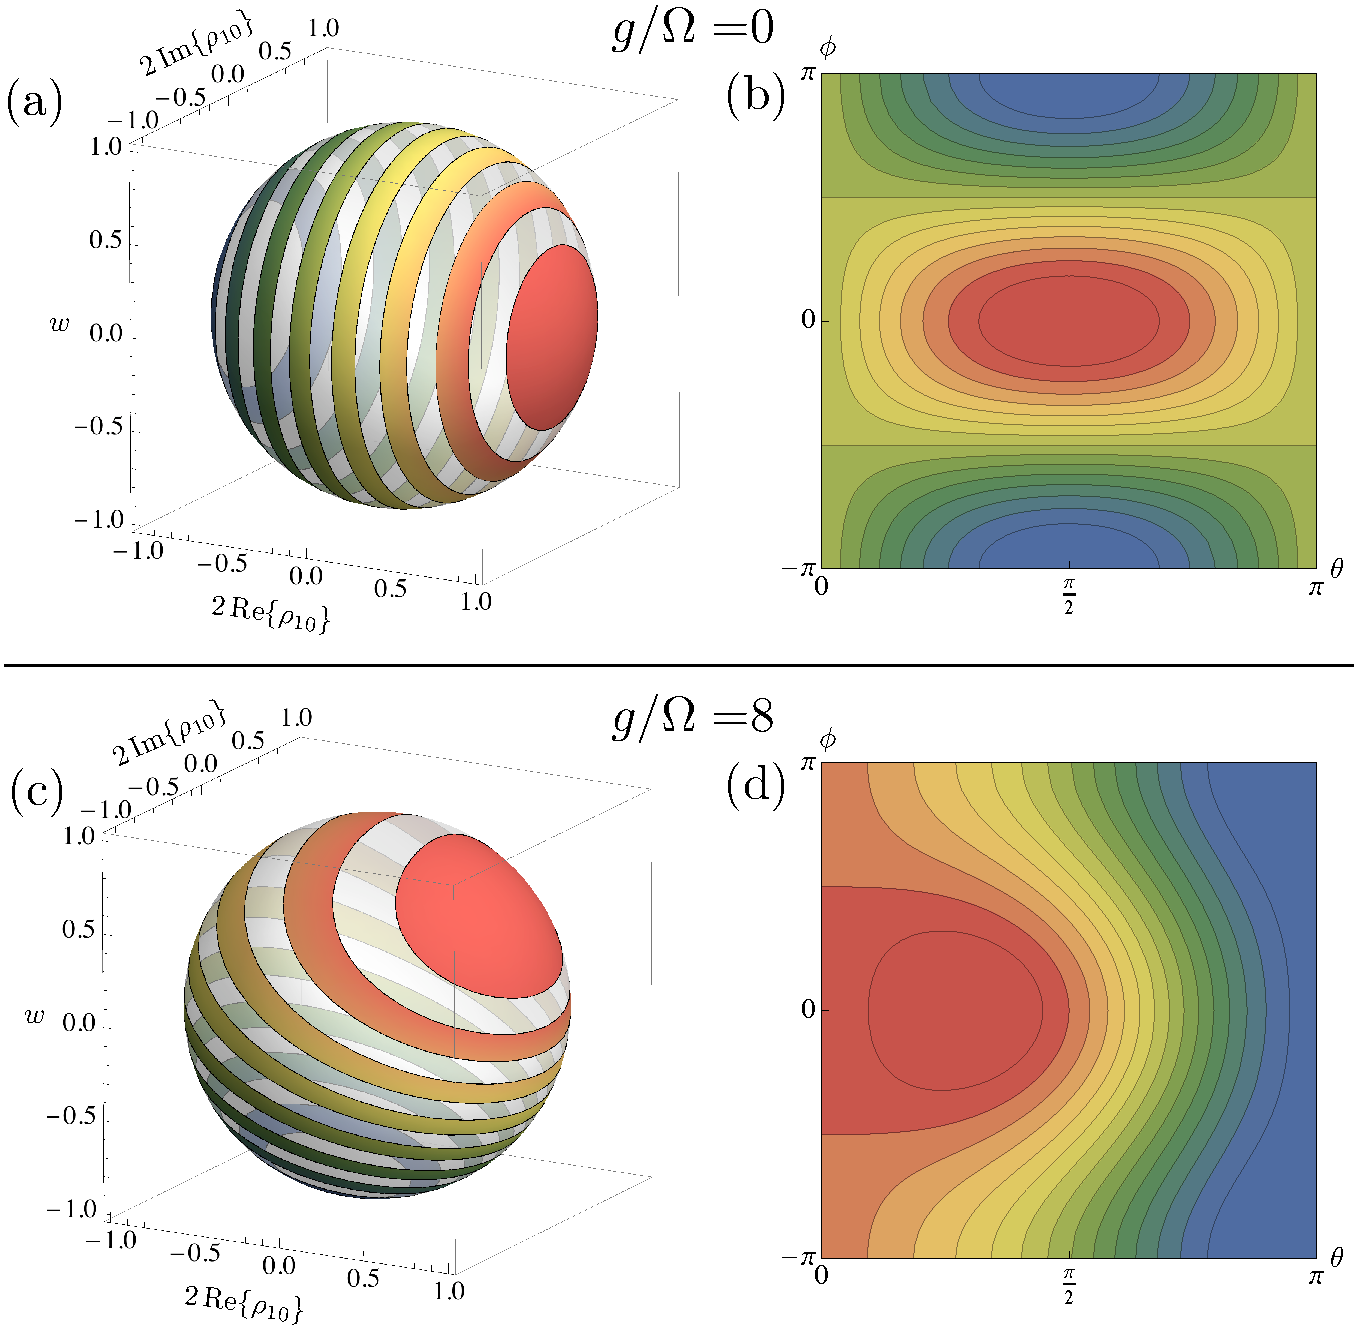
\includegraphics[width=13cm]{BlochSpheres}
    \caption{Bloch sphere representation of the evolution described by \eqref{Peaks:OpticalBlochEquations}. The upper figures (a) and (b) represent the case of the usual optical Bloch equations with no damping ($g/\Omega=0$), middle figures (c) and (d) illustrate the effect of the nonlinear term on the evolution with $g/\Omega = 8$, and the lower figures (e) and (f) illustrate the limit where the nonlinear term dominates ($g/\Omega \rightarrow \infty$). The left figures (a), (c), (e) illustrate the Bloch sphere coloured according to the energy per particle $E$ [see~\eqref{Peaks:OpticalBlochEnergy}]. The system is constrained to move on lines of constant colour. Bands have been removed from these spheres for illustration purposes only. The right figures (b), (d), (f) are contour plots of the energy per particle $E$ over the surface of the Bloch sphere.
     \label{Peaks:BlochSphere}}
\end{figure}

\subsection{Excitation dynamics}

The evolution of small perturbations about the mean-field dynamics of a condensate define both the excitation spectrum of the condensate and its stability to perturbations. 
%These perturbations not only arise from experimental uncertainties, but are an  inescapable consequence of quantum mechanics due to the fluctuations of the vacuum itself.
To determine the evolution of these excitations the mean-field dynamics must be separated from that of the excitations. To this aim we define the deviation operators $\delta\hat{\Psi}_i = \hat{\Psi}_i - \mean{\hat{\Psi}_i}$ and treat $\delta\hat{\Psi}_i$ as a small quantity. In this case the $\mean{\hat{\Psi}_i}=\Psi_i$ are themselves time dependent, obeying the equations for the mean-field \eqref{Peaks:MeanFieldEquationsOfMotion}.

The equations of motion for the deviation operators are obtained by replacing the field operators $\hat{\Psi}_i$ in the operator evolution equations \eqref{Peaks:OperatorEquationsOfMotion} with $\Psi_i + \delta \hat{\Psi}_i$ and keeping only terms up to first order in the deviation operators. Applying this procedure gives
\begin{subequations}
    \label{Peaks:DeviationOperatorsEvolutionXSpace}
    \begin{align}
        \begin{split}
            i \hbar \frac{\partial }{\partial t}\delta \hat{\Psi}_1 =& U\left[ \left(2\abs{\Psi_1}^2+\abs{\Psi_0}^2 \right)\delta \hat{\Psi}_1 + \Psi_1^2\delta\hat{\Psi}_1^\dagger + \Psi_1\Psi_0\delta\hat{\Psi}_0^\dagger + \Psi_0^*\Psi_1\delta\hat{\Psi}_0\right]\\
                    & - \frac{\hbar^2}{2M}\nabla^2 \delta \hat{\Psi}_1 +\hbar \Omega\delta\hat{\Psi}_0- \mu \delta \hat{\Psi}_1,
        \end{split}\\
        \begin{split}
        i \hbar \frac{\partial }{\partial t}\delta \hat{\Psi}_0 =& U\left[\left(2\kappa \abs{\Psi_0}^2 +\abs{\Psi_1}^2\right)\delta\hat{\Psi}_0 + \kappa \Psi_0^2 \delta\hat{\Psi}_0^\dagger + \Psi_1\Psi_0\delta\hat{\Psi}_1^\dagger + \Psi_1^*\Psi_0\delta\hat{\Psi}_1\right]\\
                    & -\frac{\hbar^2}{2M}\nabla^2 \delta \hat{\Psi}_0 +\hbar \Omega\delta\hat{\Psi}_1 - \mu \delta\hat{\Psi}_0.
        \end{split}
    \end{align}
\end{subequations}

Having assumed the mean-field (but not the fluctuations) to be homogenous, the evolution equations are spatially translation-invariant and will take their simplest form in a Fourier basis. Performing the Fourier transform of \eqref{Peaks:DeviationOperatorsEvolutionXSpace} yields
\begin{subequations}
    \label{Peaks:DeviationOperatorsEvolutionKSpace}
    \begin{align}
        \begin{split}
            i \hbar \frac{\partial }{\partial t}\delta \hat{\Psi}_1(\vect{k}) =& U\left[ \left(2\abs{\Psi_1}^2+\abs{\Psi_0}^2 \right)\delta \hat{\Psi}_1(\vect{k}) + \Psi_1^2\delta\hat{\Psi}_1^\dagger(-\vect{k}) + \Psi_1\Psi_0\delta\hat{\Psi}_0^\dagger(-\vect{k}) + \Psi_0^*\Psi_1\delta\hat{\Psi}_0(\vect{k})\right]\\
                    & +\frac{\hbar^2 \vect{k}^2}{2M} \delta \hat{\Psi}_1(\vect{k}) +\hbar \Omega\delta\hat{\Psi}_0(\vect{k})- \mu \delta \hat{\Psi}_1(\vect{k}),
        \end{split}\\
        \begin{split}
        i \hbar \frac{\partial}{\partial t} \delta \hat{\Psi}_0(\vect{k}) =& U\left[\left(2\kappa \abs{\Psi_0}^2 +\abs{\Psi_1}^2\right)\delta\hat{\Psi}_0(\vect{k}) + \kappa \Psi_0^2 \delta\hat{\Psi}_0^\dagger(-\vect{k}) + \Psi_1\Psi_0\delta\hat{\Psi}_1^\dagger(-\vect{k}) + \Psi_1^*\Psi_0\delta\hat{\Psi}_1(\vect{k})\right]\\
                    & +\frac{\hbar^2 \vect{k}^2}{2M} \delta \hat{\Psi}_0(\vect{k}) +\hbar \Omega\delta\hat{\Psi}_1(\vect{k}) - \mu \delta\hat{\Psi}_0(\vect{k}).
        \end{split}
    \end{align}
\end{subequations}

In this form, it is clear that the Fourier modes are almost completely decoupled from each other. Each deviation operator $\delta\hat{\Psi}_i(\vect{k})$ is only coupled to $\left\{\delta\hat{\Psi}_j(\vect{k}),\, \delta\hat{\Psi}_j^\dagger(-\vect{k})\right\}$, with each $\delta\hat{\Psi}_i^\dagger(-\vect{k})$ also only coupled to this same set. This can be exploited to write the equations \eqref{Peaks:DeviationOperatorsEvolutionKSpace} in matrix form as
\begin{align}
    \label{Peaks:DeviationOperatorsMatrixEvolution}
    i \hbar \frac{\partial }{\partial t}\hat{\vect{\Upsilon}}(\vect{k}) &= \mathcal{H}(\vect{k}) \hat{\vect{\Upsilon}}(\vect{k}),
\end{align}
where
\begin{align}
    \hat{\vect{\Upsilon}}(\vect{k}) &= 
    \begin{pmatrix}
        \delta\hat{\Psi}_1(\vect{k}) &
        \delta\hat{\Psi}_1^\dagger(-\vect{k}) &
        \delta\hat{\Psi}_0(\vect{k}) &
        \delta\hat{\Psi}_0^\dagger(-\vect{k})
    \end{pmatrix}^\text{T},\\
    \mathcal{H}(\vect{k}) &= 
    \begin{pmatrix}
        \varepsilon(\vect{k}) + q_{1} - \mu & v_{11} & u_{01} + \hbar \Omega & v_{10}\\
        -v_{11}^* & -\varepsilon(\vect{k}) - q_1 + \mu & -v_{10}^* & -u_{10} - \hbar \Omega\\
        u_{10} + \hbar \Omega & v_{10} & \varepsilon(\vect{k}) + q_0 - \mu & \kappa v_{00}\\
        -v_{10}^* & -u_{01} - \hbar \Omega & -\kappa v_{00}^* & -\varepsilon(\vect{k}) - q_0 + \mu
    \end{pmatrix},\label{Peaks:HMatrix}
\end{align}
and $q_1 = U\left(2\abs{\Psi_1}^2+\abs{\Psi_0}^2\right)$, $q_0 = U\left(2\kappa \abs{\Psi_0}^2 + \abs{\Psi_1}^2\right)$, $u_{ij} = U\Psi_i^*\Psi_j$, $v_{ij} = U\Psi_i\Psi_j$, and $\displaystyle \protect{\varepsilon(\vect{k}) = \frac{\hbar^2 \vect{k}^2}{2M}}$.

Note that the matrix $\mathcal{H}(\vect{k})$ is not the Hamiltonian, but is related to it by \eqref{Peaks:ScriptHRelationshipToHamiltonian}. As a consequence, although it will be shown later that in some circumstances $\mathcal{H}(\vect{k})$ contains complex eigenvalues and is hence not Hermitian, this in no way conflicts with the requirement that the Hamiltonian $\hat{H}$ must be Hermitian and only have real eigenvalues.

If the coefficients of the matrix $\mathcal{H}(\vect{k})$ were not time-dependent, the excitation spectrum of the condensate could simply be obtained from the eigenvalues of $\mathcal{H}(\vect{k})$. Non-zero imaginary components for these eigenvalues would indicate the corresponding mode to be unstable\footnote{This is true independent of the sign of the imaginary component as the eigenvalues come in pairs with opposite imaginary components. A full discussion of this issue is given in \appendixref{FloquetAppendix}.}. Before continuing with the general case of $\kappa \neq 1$, in the next section the limit in which all scattering lengths are equal ($\kappa=1$) will be considered and some familiar results recovered.

\subsection{Excitation spectra in the $\kappa = 1$ limit}
\label{Peaks:Kappa1Limit}
In the limit that all the scattering lengths are the same ($\kappa = 1$), the nonlinear term in \eqref{Peaks:MeanFieldEquationsOfMotion} only contributes to a rotation of the global phase of the spinor condensate. In this case the dynamics can be solved analytically and familiar excitation spectra recovered.

The general solution to \eqref{Peaks:MeanFieldEquationsOfMotion} for $\kappa = 1$ is
\begin{subequations}
    \label{Peaks:Kappa1MeanFieldSolution}
    \begin{align}
        \Psi_1(t) &= \cos(\Omega t) \Phi_+ + \sin(\Omega t) \Phi_-, \\
        \Psi_0(t) &= -i\sin(\Omega t) \Phi_+ + i\cos(\Omega t) \Phi_-,
    \end{align}
\end{subequations}
for some complex constants $\Phi_\pm$, and where the chemical potential $\mu = n U$ has cancelled the global phase rotation. This solution can be viewed as a linear basis transformation from $\hat{\Psi}_i$ to $\hat{\Phi}_\pm$, which are the eigenvectors of the Rabi coupling term in \eqref{Peaks:InitialHamiltonian}. Performing this change of basis on the original Hamiltonian \eqref{Peaks:InitialHamiltonian} yields a Hamiltonian of the same form, but without the Rabi coupling term. The equations of motion for the deviation operators $\delta\hat{\Phi}_\pm$ therefore give a matrix of precisely the same form as \eqref{Peaks:HMatrix} but in terms of $\Phi_\pm$ and $\delta\hat{\Phi}_\pm$ instead of the $\Psi_i$ and $\delta\hat{\Psi}_i$, and with $\Omega$ replaced by 0. This new matrix $\mathcal{H}'(\vect{k})$ is time-independent and can be diagonalised to give the eigenvalues
\begin{subequations}
    \label{Peaks:Kappa1Eigenvalues}
    \begin{align}
        \hbar \omega_\uparrow(\vect{k}) &= \sqrt{\varepsilon(\vect{k})\left(\varepsilon(\vect{k}) + 2 n U\right)},\\
        \hbar \omega_\downarrow(\vect{k}) &= \varepsilon(\vect{k}),
    \end{align}
\end{subequations}
where $\displaystyle\varepsilon(\vect{k}) = \frac{\hbar^2\vect{k}^2}{2M}$, $n= \abs{\Psi_1}^2 + \abs{\Psi_0}^2$ and the remaining two eigenvalues are the negatives of \eqref{Peaks:Kappa1Eigenvalues}. The first of these, $\hbar \omega_\uparrow(\vect{k})$, is the usual Bogoliubov spectrum~\citep{Bogoliubov:1947} corresponding to excitations in the total condensate density. The second eigenvalue $\hbar \omega_\downarrow(\vect{k})$ is the free particle spectrum; this excitation only changes the relative densities of the two states without affecting the total density, hence not affecting the nonlinear term in the Hamiltonian \eqref{Peaks:InitialHamiltonian}.

The Hamiltonian for the condensate excitations that corresponds to the eigenvalues \eqref{Peaks:Kappa1Eigenvalues} is (refer to \sectionref{Peaks:ElementaryExcitations})
\begin{align}
    \hat{H} &= \sum_{i=\uparrow,\downarrow}\int d\vect{k}\, \hbar \omega_i(\vect{k}) \hat{\Lambda}_i^\dagger(\vect{k}) \hat{\Lambda}_i^{\phantom{\dagger}}(\vect{k}),
\end{align}
where the $\hat{\Lambda}_{\uparrow,\downarrow}(\vect{k})$ obey boson commutation relations and are the corresponding normalised eigenvectors to the eigenvalues in \eqref{Peaks:Kappa1Eigenvalues}. The normalised eigenvectors for the negatives of those eigenvalues are the $\hat{\Lambda}_{\uparrow, \downarrow}^\dagger(-\vect{k})$.

\subsection[Floquet's theorem]{Floquet's theorem~\citep[\S 3.2]{AppliedNonlinearDynamics}}
\label{Peaks:FloquetsTheorem}

Having considered the limit of equal scattering lengths, it now remains to determine the energy spectrum and condensate stability in the general case of $\kappa \neq 1$. Analytic results cannot be obtained in this limit, but numeric results corresponding to the experimental situation in \sectionref{Peaks:ExperimentalSetup} can be obtained.

In the general case, the excitation spectrum cannot be obtained from the eigenvalues of the matrix $\mathcal{H}(\vect{k})$ in \eqref{Peaks:HMatrix} as the matrix's entries are themselves time-dependent. However, due to the periodicity of the mean-field wavefunctions demonstrated in \sectionref{Peaks:MeanFieldPeriodicity}, the entries of $\mathcal{H}(\vect{k})$ are themselves periodic, which enables Floquet's theorem to be applied.

Floquet's theorem proves that the matrix solution to the initial-value problem
\begin{subequations}
    \label{Peaks:FloquetMatrixIVP}
    \begin{align}
        \frac{d}{dt}\vect{\Pi}(t) &= \vect{A}(t) \vect{\Pi}(t),\\
        \vect{\Pi}(0) &= \mathbb{I},
    \end{align}
\end{subequations}
where $\mathbb{I}$ is the $n \times n$ identity matrix and $\vect{A}(t)$ a periodic $n \times n$ matrix with period $T$ can be written in the form
\begin{align}
    \vect{\Pi}(t) = \vect{P}(t) \exp(-i\vect{Q} t),
    \label{Peaks:FloquetSolution}
\end{align}
for some constant matrix\footnote{There are differing definitions of the matrix $\vect{Q}$. While it is usual in quantum mechanics literature~\citep{Shirley:1965,Hanggi:1998,Garrison:1999} to define \eqref{Peaks:FloquetSolution} with the $-i$ in the exponent,  in mathematics literature~\citep{Moulton:1958,AppliedNonlinearDynamics} the $-i$ is omitted.} $\vect{Q}$ and $\vect{P}(t)$ a matrix of periodic functions with period $T$ and $\vect{P}(0) = \mathbb{I}$. The matrix solution $\vect{\Pi}(t)$ is the general solution to the related linear system
\begin{align}
    \frac{d}{dt}\vect{x}(t) &= \vect{A}(t) \vect{x}(t),
    \label{Peaks:FloquetVectorIVP}
\end{align}
for any initial condition $\vect{x}(0)$ where $\vect{x}(t)$ is a vector. Every solution $\vect{x}(t)$ to this problem can be written in terms of the matrix $\vect{\Pi}(t)$ using
\begin{align}
    \vect{x}(t) &= \vect{\Pi}(t) \vect{x}(0),
\end{align}
as is easily verified. The matrix solution $\vect{\Pi}(t)$ thus completely determines the behaviour of all solutions to \eqref{Peaks:FloquetVectorIVP}.

The eigenvalues of $\vect{Q}$ are known as \emph{Floquet exponents} (or \emph{characteristic exponents}) and determine the long-term growth or decay of the solutions to \eqref{Peaks:FloquetVectorIVP}. These eigenvalues can be obtained from the \emph{monodromy matrix},
\begin{align}
    \label{Peaks:MonodromyMatrix}
    \mathcal{M} &= \vect{\Pi}(T) = \exp(-i\vect{Q} T),
\end{align}
as $\vect{P}(T) = \vect{P}(0) = \mathbb{I}$. The existence and uniqueness of the solution to \eqref{Peaks:FloquetMatrixIVP} guarantees that $\vect{\Pi}(t)$ and hence $\mathcal{M}$ will be invertible. The Floquet exponents $\xi_i$ can therefore be obtained from the eigenvalues $\lambda_i$ of the monodromy matrix using $\lambda_i = \exp(-i\xi_i T)$.\footnote{Note that the Floquet exponents are only defined modulo $2 \pi/T$ as $\displaystyle\lambda = \exp(-i\xi T) = \exp\left[-i \left(\xi + n \frac{2 \pi}{T}\right)T\right]$ for any integer $n$.} It is the Floquet exponents of the matrix $\mathcal{H}(\vect{k})$ that we wish to calculate in order to determine the stability of the condensate to excitations.

\subsection{Determination of the dynamical instabilities}
\label{Peaks:ExperimentEigenvalues}

The method outlined in the previous section for determining the Floquet exponents of the system \eqref{Peaks:DeviationOperatorsMatrixEvolution} requires knowledge of its period $T$, and hence the period of the mean field dynamics given by \eqref{Peaks:MeanFieldEquationsOfMotion}. Although this period cannot be determined analytically, it can be found numerically.

It was shown in \sectionref{Peaks:MeanFieldPeriodicity} that up to a global phase rotation $\displaystyle f(T) = e^{i 2\pi \Delta \nu T}f(0)$, the mean fields $\Psi_j(t)$ are periodic. The mean fields $\Psi_j(t)$ can be therefore written in the form
\begin{align}
    \label{Peaks:MeanFieldFourierDecomposition}
    \Psi_j(t) = \sum_{n=-\infty}^\infty \alpha_{j,n} \exp\left[i 2\pi \left( n \nu_0 + \Delta\nu\right)t \right],
\end{align}
for some complex constants $\alpha_{j, n}$, fundamental frequency $\nu_0 = T^{-1}$, and frequency offset $\Delta \nu$. In this form, the $\Psi_j(t)$ are not exactly periodic as $\Psi_j(T) = \exp(i\Delta \nu T)\Psi_j(0)$, but this frequency offset can be cancelled by an appropriate choice of the energy offset $\mu = -2 \pi \hbar\Delta \nu$ in \eqref{Peaks:InitialHamiltonian}.

The period $T$ and frequency offset $\Delta\nu$ in \eqref{Peaks:MeanFieldFourierDecomposition} can be determined from the Fourier transform of $\Psi_j(t)$, which will have sharp peaks at the frequencies $n \nu_0 + \Delta \nu$ (see \figureref{Peaks:MeanFieldFourierTransform}). Choosing the energy offset $\mu=-2 \pi \hbar \Delta\nu$, the frequency offset in \eqref{Peaks:MeanFieldFourierDecomposition} can be cancelled making the $\Psi_j(t)$ with this energy offset exactly periodic with period $T$. \figureref{Peaks:MeanFieldFourierTransform} illustrates the Fourier transform of the numerical solutions for $\Psi_j(t)$ for a Rabi frequency of $\Omega = 2 \pi \times \unit[3]{kHz}$ from which the period $T=\unit[150]{\micro{}s}$ and frequency offset $\Delta \nu = \unit[-1.78]{kHz}$ have been obtained.

\begin{figure}
    \centering
    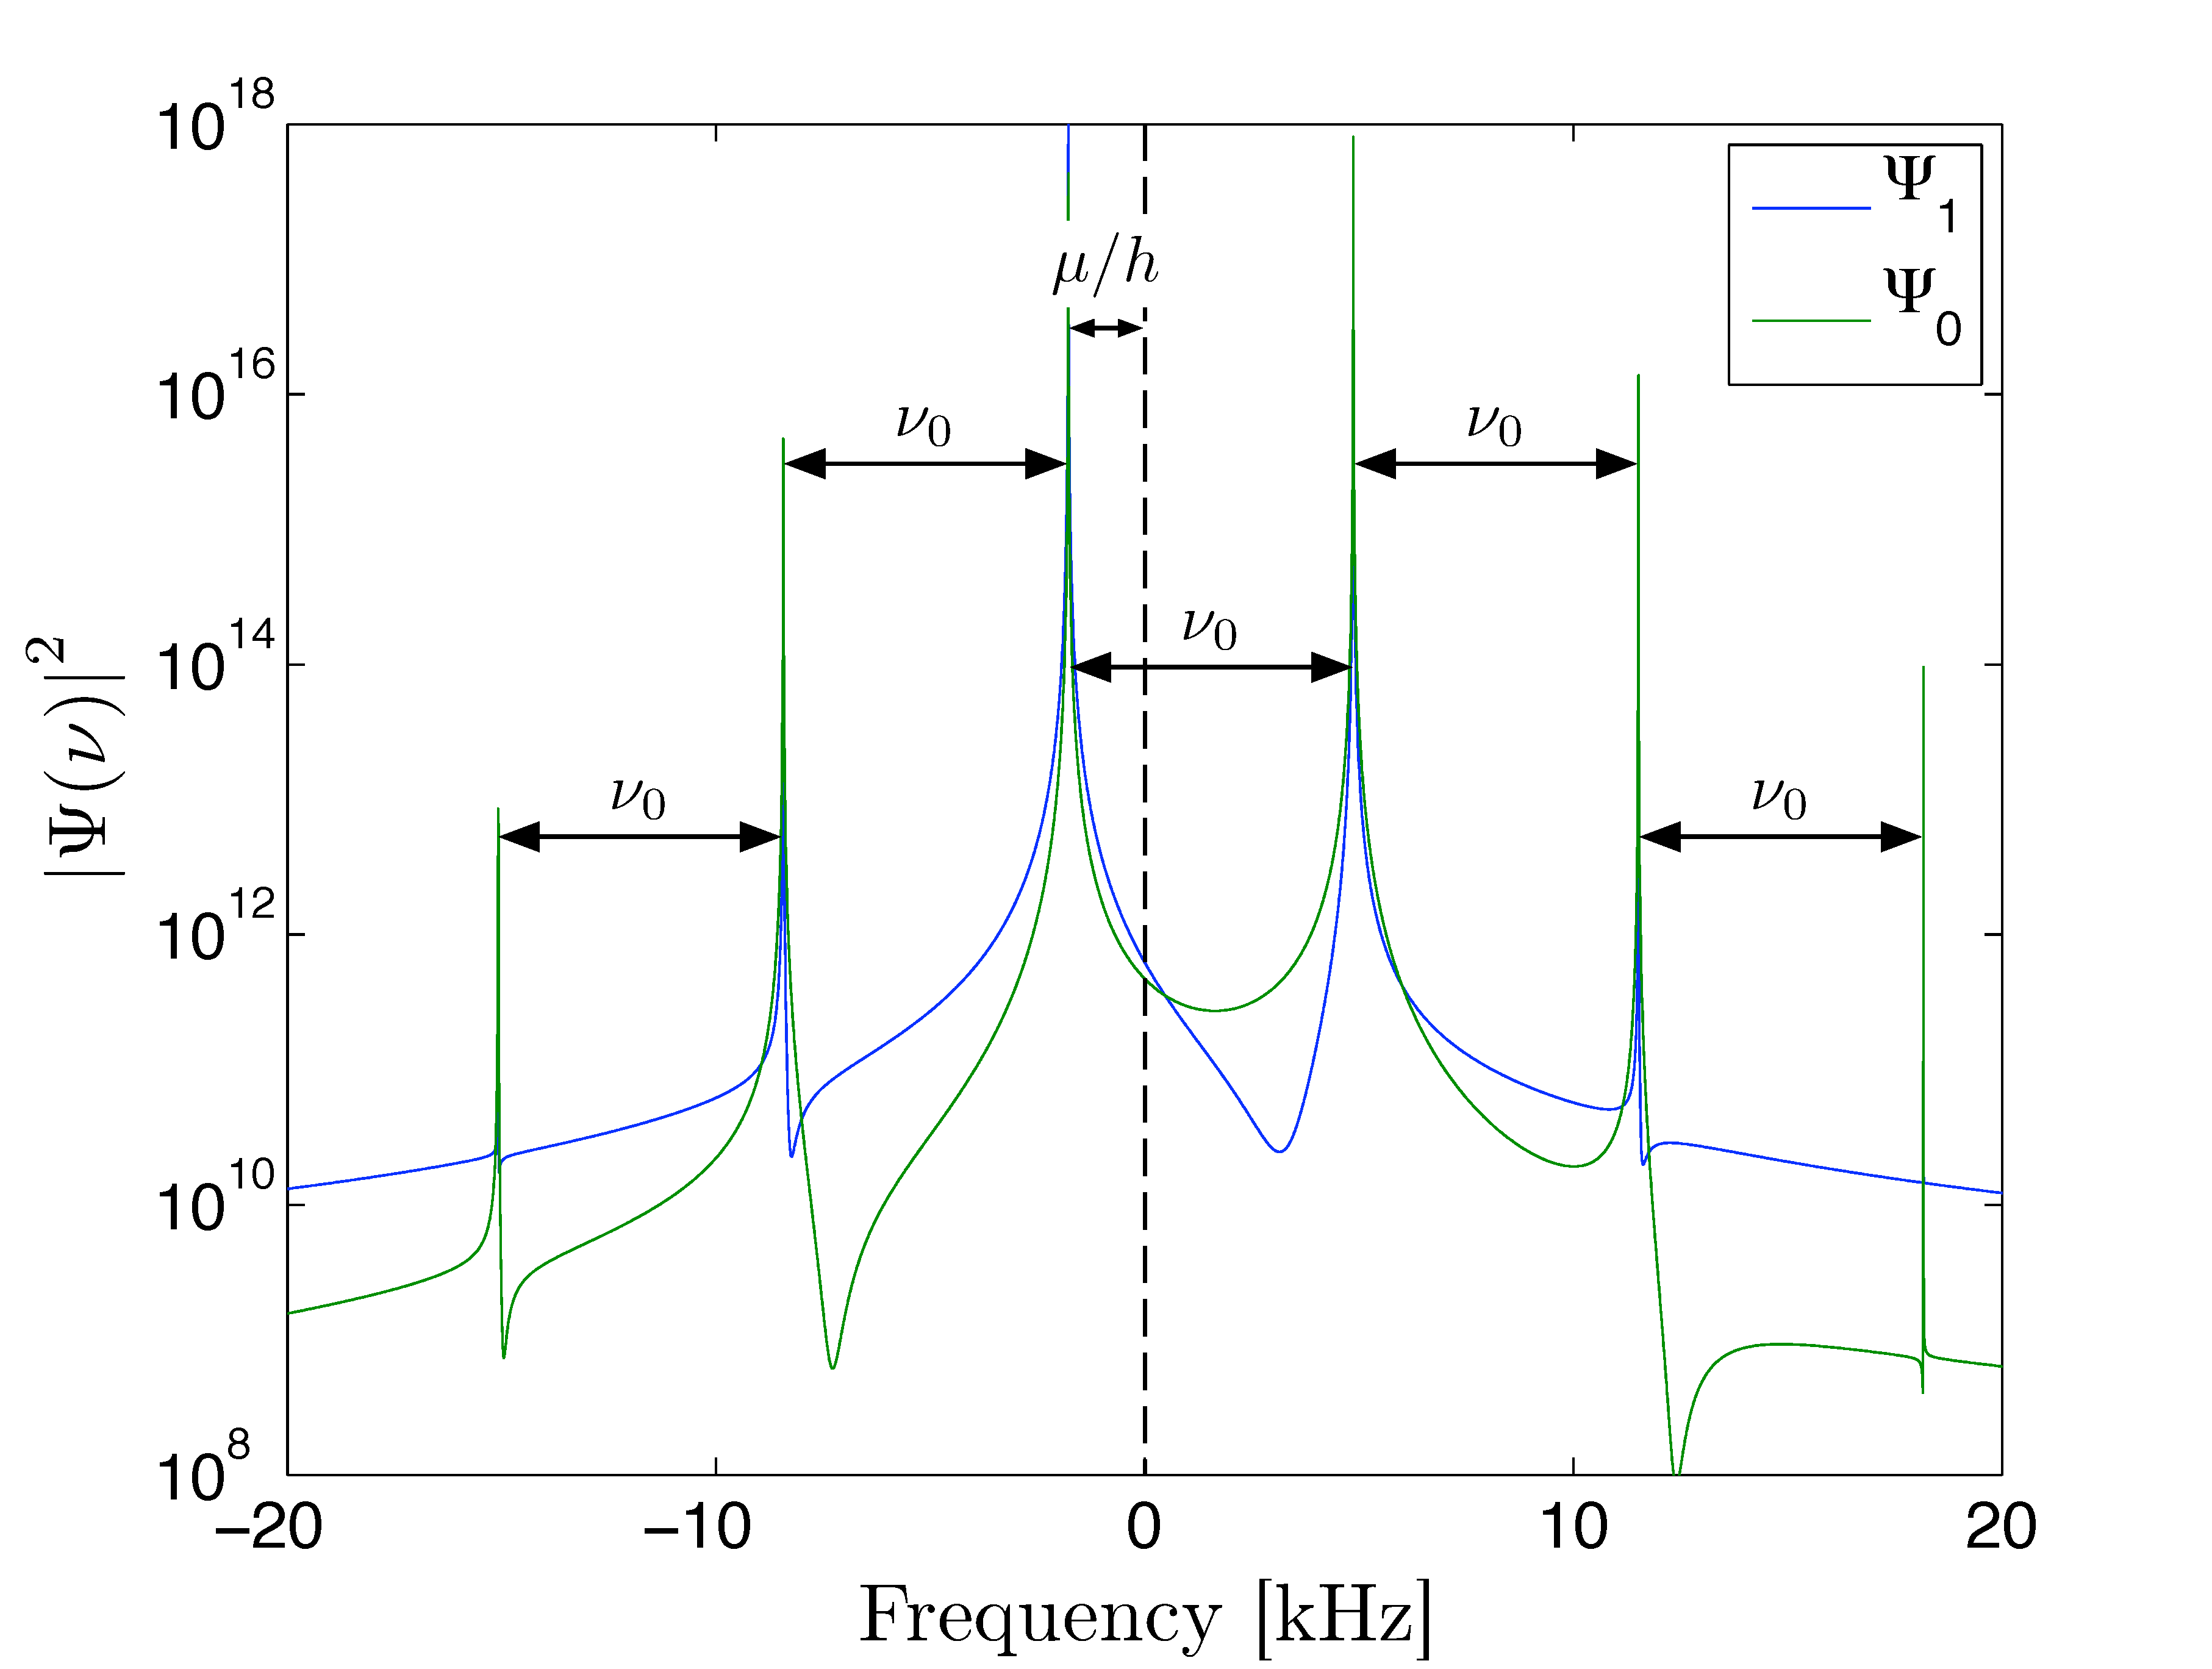
\includegraphics[width=14cm]{MeanFieldFourierTransform}
    \caption{Temporal Fourier transform of the calculated mean field evolution defined by \eqref{Peaks:MeanFieldEquationsOfMotion} for the centre of the condensate defined by the experimental parameters given in \tableref{Peaks:ExperimentalParameters}. The frequency $\nu_0$ is the inverse period of the system, and $\Delta\nu$ represents the global phase rotation. From the data in this figure the values $\nu_0 = \unit[6.65]{kHz}$ and $\Delta\nu = \unit[-1.78]{kHz}$ can be determined, giving the period as $T=\unit[150]{\micro{}s}$. \label{Peaks:MeanFieldFourierTransform}}
\end{figure}

The period and energy offset determined, it remains to calculate the mono\-dromy matrix $\mathcal{M}(\vect{k})$ from which the Floquet exponents may be derived. This is achieved by numerically solving the related matrix problem to \eqref{Peaks:DeviationOperatorsMatrixEvolution} from $t=0$ to $t=T$ [refer to \eqref{Peaks:MonodromyMatrix}]. Noting that the matrix $\mathcal{H}(\vect{k})$ only depends on $k = \abs{\vect{k}}$, the solutions for the Floquet exponents $\xi(\vect{k}) = \omega(\vect{k}) + i\gamma(\vect{k})$ are illustrated in \figureref{Peaks:CondensateEigenvalues}.

In the limit that the mean-field is time-independent (a degenerate case of periodicity), the Floquet exponents $\xi(\vect{k})$ are related to the eigenvalues $\lambda(\vect{k})$ of the matrix $\mathcal{H}$ by $\xi(\vect{k}) = \lambda(\vect{k}) / \hbar$. It was previously stated that eigenvalues of $\mathcal{H}(\vect{k})$ with nonzero imaginary components would be unstable, this is also true for the Floquet exponents $\xi(\vect{k})$.

\begin{figure}
    \centering
    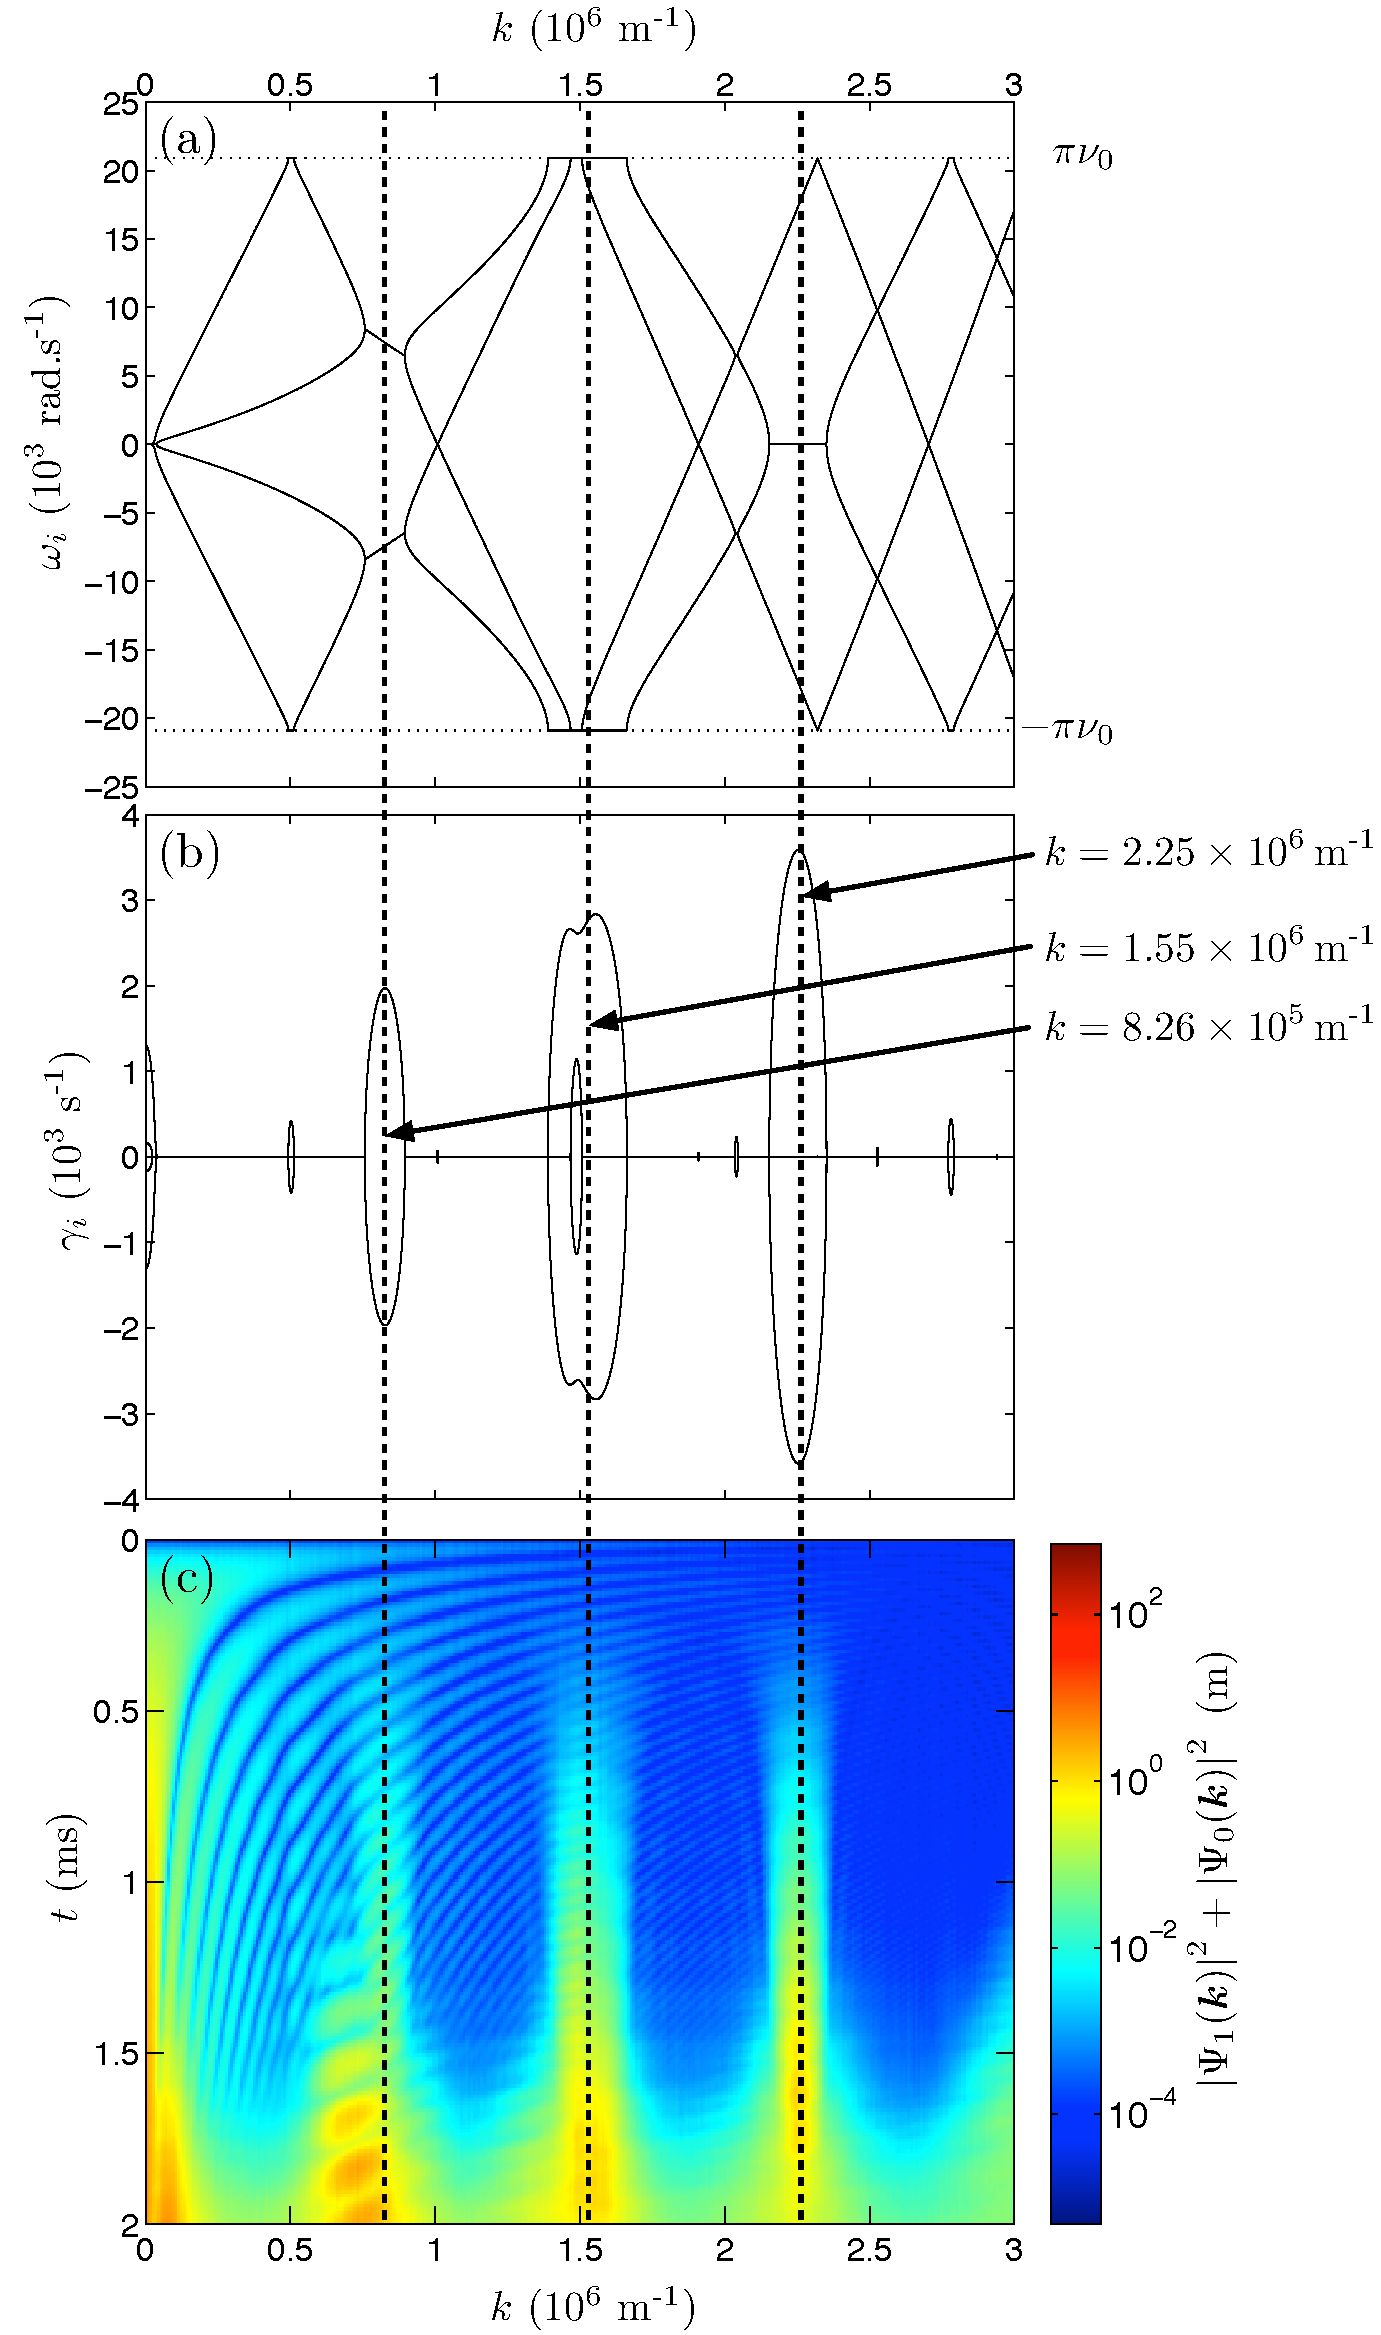
\includegraphics[height=19cm]{CondensateEigenvalues}
    \caption{Illustration of the Floquet exponents for $\mathcal{H}(\vect{k})$ and comparison to a corresponding truncated Wigner simulation for $\Omega = 2\pi \times \unit[3]{kHz}$.
        Upper figure (a) displays the real part $\omega_i$ of the Floquet exponents. As the $\omega_i$ can only be determined up to a multiple of $2\pi\nu_0$ [see \eqref{Peaks:AmbiguityFloquetExponent}], they have been reduced modulo $2\pi\nu_0$ into the range $\left[-\pi\nu_0,\, \pi\nu_0\right]$.
        The middle figure (b) shows the imaginary part $\gamma_i$ of the Floquet exponents, which indicate an instability for the corresponding wavenumber when they are nonzero.  Note that what appears to be a horizontal line at $\gamma_i=0$ is not an axis, but a plot of the $\gamma_i$ which are mostly zero.
        Lower figure (c) shows the results of a 1D truncated Wigner simulation corresponding to the system under consideration in (a) and (b). The truncated Wigner simulation exhibits growth in the same modes predicted from the results of the perturbative analysis shown in (b). The truncated Wigner results shown are the average of 500 realisations.
        \label{Peaks:CondensateEigenvalues}}
\end{figure}

The temporal periodicity of the system implies that the real components $\omega_i(\vect{k})$ of the Floquet exponents are only uniquely defined modulo $2\pi \nu_0$ (see \figureref{Peaks:CondensateEigenvalues}(a)). This is because any eigenvalue $\lambda$ of the monodromy matrix $\mathcal{M}(\vect{k})$ corresponds to infinitely many Floquet exponents,
\begin{align}
    \label{Peaks:AmbiguityFloquetExponent}
    \lambda = \exp\left[-i \left(\omega + 2 \pi n \nu_0 + i \gamma\right)T\right] = \exp\left[-i\left(\omega + i \gamma\right)T\right].
\end{align}
This does not hinder our understanding of the system as our primary interest is in the stability of the condensate to excitations, which is determined by the $\gamma_i(\vect{k})$.

The normalised eigenvectors of the system are not always annihilation or creation operators; as is discussed in \appendixref{FloquetAppendix}, this is only true when the Floquet exponents are purely real. When the Floquet exponents have a nonzero imaginary component, annihilation and creation operators can be constructed from linear combinations of the eigenvectors. Not being eigenvectors, these operators will therefore have nontrivial evolution. As is shown in \appendixref{FloquetAppendix}, Floquet exponents with nonzero imaginary parts come in pairs of the form $\omega(\vect{k}) \pm i \gamma(\vect{k})$. From the corresponding eigenvectors to these Floquet exponents the bosonic annihilation operator $\hat{\Lambda}(\vect{k}, t)$ can be formed, which evolves as
\begin{subequations}
    \label{Peaks:DynamicalInstability}
    \begin{align}
        \hat{\Lambda}(\vect{k}, nT) &= e^{i n\omega(\vect{k}) T} \left( \sinh(n\gamma(\vect{k}) T) \hat{\Lambda}'^\dagger(-\vect{k}, 0) + \cosh(n\gamma(\vect{k}) T) \hat{\Lambda}(\vect{k}, 0)\right),\\
        \hat{\Lambda}'(\vect{k}, nT) &= e^{-i n \omega(\vect{k}) T} \left( \sinh(n\gamma(\vect{k}) T) \hat{\Lambda}^\dagger(-\vect{k}, 0) + \cosh(n\gamma(\vect{k}) T) \hat{\Lambda}'(\vect{k}, 0)\right),
    \end{align}
\end{subequations}
where $n$ is a positive integer, and where $\hat{\Lambda}'(\vect{k}, t)$ will be equal to $\hat{\Lambda}(\vect{k}, t)$ in some circumstances as discussed in \appendixref{FloquetAppendix}. Due to the exponential growth in \eqref{Peaks:DynamicalInstability}, the mode corresponding to $\hat{\Lambda}(\vect{k})$ represents a dynamical instability of the condensate.

The behaviour of the dynamical instabilities is governed by \eqref{Peaks:DynamicalInstability} only while the unstable modes have a small occupation compared to the condensate, and scattering between the unstable modes can be neglected. \figureref{Peaks:CondensateEigenvalues}(c) shows the results of a truncated Wigner simulation of the Hamiltonian \eqref{Peaks:InitialHamiltonian}, which is in excellent agreement with the location of the dynamical instabilities as determined by the Floquet exponents [see \figureref{Peaks:CondensateEigenvalues}(b)]. For later times, there is an additional mode undergoing growth, $k \approx \unit[7.5\times 10^5]{m}^{-1}$. This mode is the result of scattering between the dynamical instabilities, a process neglected the perturbative approach taken in this section. 

\parasep

In summary, the procedure used to find the Floquet exponents of $\mathcal{H}(\vect{k})$, and hence the stability of the condensate to excitations is:
\begin{enumerate}
    \item Numerically solve \eqref{Peaks:MeanFieldEquationsOfMotion} with $\mu=0$ for a long time $t \gg T$ where $T$ is the periodicity of the solution.
    \item Perform the temporal Fourier transform of the solutions obtained for $\Psi_i(t)$ to accurately determine the period $T$ and the value of the energy offset $\mu$ required to cancel any global phase evolution to make the wavefunctions themselves periodic (see \figureref{Peaks:MeanFieldFourierTransform}).
    \item Using the calculated period and energy offset, numerically solve the related matrix problem to \eqref{Peaks:DeviationOperatorsMatrixEvolution} for a range of values of $\vect{k}$ to obtain the monodromy matrix $\mathcal{M}(\vect{k})$. In this calculation the matrix $\vect{A}(t)$ in \eqref{Peaks:FloquetMatrixIVP} is $\displaystyle -\frac{i}{\hbar}\mathcal{H}(\vect{k}, t)$.
    \item Calculate the eigenvalues $\lambda_i$ of $\mathcal{M}(\vect{k})$ and determine the Floquet exponents $\xi_i$ using $\protect{\lambda_i = \exp(-i \xi_i T)}$ (see \figureref{Peaks:CondensateEigenvalues}). The real parts of these Floquet exponents gives the energy spectrum, with nonzero imaginary parts giving the growth rate for the corresponding instability.
\end{enumerate}

\subsection{Discussion of the dynamical instabilities}
\label{Peaks:DynamicalInstabilitiesDiscussion}

The dynamics of the dynamical instability $\hat{\Lambda}(\vect{k})$ described by \eqref{Peaks:DynamicalInstability} are the same as those of the amplified modes in non-degenerate parametric down-conversion~\citep{WallsMilburn}.  In parametric down-conversion, a non-linear crystal produces pairs of EPR-entangled\footnote{EPR entanglement was proposed by Einstein, Podolsky and Rosen~\citep{Einstein:1935} as a demonstration that quantum mechanics could not simultaneously be local, real and complete.  Their preferred option of local and real but \emph{incomplete} has since been demonstrated to be incorrect~\citep{Aspect:1982uq}.  For more information about EPR entanglement, see~\citep[Chapter 18]{Scully}.} photons at frequencies $\omega_1$ and $\omega_2$ from a classical seed beam at frequency $\omega = \omega_1 + \omega_2$.  Analogously, in the case of the He* BEC discussed at the start of this chapter, the evolution represented by \eqref{Peaks:DynamicalInstability} will result in the spontaneous formation of EPR-entangled pairs of excitations, one in each of the $\hat{\Lambda}(\pm \vect{k})$ modes. Although these modes will be entangled upon production, it does not necessarily follow that parts of the outcoupled atom laser will be entangled; the entangled $\hat{\Lambda}(\vect{k})$ modes are each superpositions of $m_F=1$ and $m_F=0$ states, but only the $m_F=0$ atoms can leave the condensate. However, if the $m_F=1$ components of the entangled modes are outcoupled faster than the time to undergo half an oscillation in the trap and reverse their momenta ($\unit[9]{ms}$), then number difference squeezing between the atom laser components with opposite axial momenta may be observed.

The unstable excitations would not necessarily be expected to form along the tight trapping directions. Of the three most unstable modes in \figureref{Peaks:CondensateEigenvalues}, the shortest wavelength for these excitations is $\lambda \approx \unit[3]{\micro m}$ which is not significantly smaller than the Thomas-Fermi radius in this dimension of $\rho_\text{TF} = \unit[9.4]{\micro m}$. Hence the local density approximation will not be satisfied in this dimension as the condensate density decays to zero over a distance a few times larger than the size of the excitation itself.  However, as the Thomas-Fermi radius in the axial dimension is $z_\text{TF} = \unit[175]{\micro m}$, the local density approximation will be a good approximation for describing the excitations along that dimension. Therefore excitations should form along the axial dimension.

This effect also depends on the scattering length for collisions between $m_F=0$ atoms being significantly smaller than both the 1--1 and 1--0 scattering lengths as no instabilities were found in the $\kappa = 1$ limit (see \sectionref{Peaks:Kappa1Limit}). 
Consequently, this effect would not be expected to be observed in atoms like $\nucl{87}{Rb}$ for which $\kappa = 1.002$~\citep{Kempen:2002,Widera:2006}.

Verification that the $\hat{\Lambda}(\vect{k})$ quasiparticles are the origin of the peak-like structure observed in the experiment required a full 3D field calculation, which is discussed in \sectionref{Peaks:3DCalculation}.  The argument made in this section that the observed structure is due to the formation of pairs of quasiparticles driven by a spontaneous four-wave mixing process indicates that a Gross-Pitaevskii model will be unable to reproduce the observations. Such a mean-field model will be insufficient due to the absence of the vacuum fluctuations which are critical to all spontaneous processes.

\section{Full 3D calculation}
\label{Peaks:3DCalculation}
In the previous section it was found that the process of outcoupling from the He* BEC discussed in \sectionref{Peaks:ExperimentalSetup} results in certain modes within the condensate becoming unstable. It was argued that these instabilities are the original cause of the observed structure in \figureref{Peaks:ExperimentalResults}. However, it is not immediately clear that these instabilities will not be suppressed by Penning ionisation which causes $m_F=0$ atoms to ionise but not pure samples of $m_F=1$ atoms (see \sectionref{BackgroundTheory:PenningIonisation} and \appendixref{PenningIonisationAppendix}). To verify that the instabilities are not suppressed and that they do cause the observed structure, a detailed numerical simulation of the experiment was performed.

The master equation that describes the experiment described in \sectionref{Peaks:ExperimentalSetup} is given by
\begin{align}
    \label{Peaks:MasterEquation}
    \frac{d }{d t}\hat{\rho} &= \frac{-i}{\hbar} [\hat{H},\, \hat{\rho} ] + \frac{9}{2} K^\text{(unpol)}_{^{4}\text{He}} \int d \vect{x}\, \mathcal{D}\left[\hat{\Xi}_{S=0,m_S=0} \right] \hat{\rho},
\end{align}
where $\displaystyle\hat{\Xi}_{S, m_S}$ is the annihilation operator for the quasimolecular state with total hyperfine spin $S$ and projection $m_S$, $\mathcal{D}[\hat{c}]\hat{\rho} \equiv \hat{c}\hat{\rho}\hat{c}^\dagger - \frac{1}{2}(\hat{c}^\dagger \hat{c} \hat{\rho} + \hat{\rho} \hat{c}^\dagger \hat{c})$ is the usual decoherence superoperator, and the second term\footnote{The reason for the difference between the ${54}/{5}$ factor in~\citet{Dall:2009} and the $9/2$ factor in \eqref{Peaks:MasterEquation} is a difference of a factor of $\sqrt{2}$ in the definition of $\hat{\Psi}_{J=0}^{\text{(mol)}}$ in~\citep{Dall:2009} and $\displaystyle\hat{\Xi}_\ket{S=0, m_S=0}$ here, and a calculational error of the order of 20\% in~\citep{Dall:2009}.} on the RHS in \eqref{Peaks:MasterEquation} is due to Penning ionisation (refer to \sectionref{BackgroundTheory:PenningIonisation} and \appendixref{PenningIonisationAppendix}) with $K^\text{(unpol)}_{^{4}\text{He}}=\unit[7.7\times 10^{-17}]{m\textsuperscript{3}s\textsuperscript{-1}}$ the Penning ionisation rate for an unpolarised thermal sample of He*~\citep{Stas:2006kx}. The Hamiltonian in \eqref{Peaks:MasterEquation} is given by
\begin{align}
    \label{Peaks:3DHamiltonian}
    \begin{split}
    \hat{H} &= \sum_i \int d\vect{x}\, \hat{\Psi}_i^\dagger \left(\frac{-\hbar^2 \nabla^2}{2 M} + V_i(\vect{x})\right)\hat{\Psi}_i^{\phantom{\dagger}} + \frac{1}{2}\sum_{S, m_S} g_{S}\int d\vect{x}\, \hat{\Xi}_{S, m_S}^\dagger \hat{\Xi}_{S, m_S}^{\phantom{\dagger}}\\
            &\phantom{=} + \sqrt{2} \hbar \Omega \sum_{i j}\int d\vect{x}\, \hat{\Psi}_i^\dagger \left(\delta_{i, j+1} + \delta_{i, j-1}\right) \hat{\Psi}_j^{\phantom{\dagger}},
    \end{split}
\end{align}
$\displaystyle \hat{\Psi}_i$ is the annihilation operator for the atomic state $\displaystyle \ket{F=1, m_F=i}$, $V_i(\vect{x})$ is the potential experienced by that state, and $g_S = 4 \pi \hbar^2 a_S/M$ is the nonlinear interaction strength, and $a_S$ is the $s$-wave scattering length for the total hyperfine spin $S$ channel (refer to \sectionref{BackgroundTheory:AtomicScattering}). The quasi-molecular annihilation operator $\displaystyle \hat{\Xi}_{S, m_S}$ is defined in terms of the atomic annihilation operators and the appropriate Clebsch-Gordan coefficients~\citep{Ho:1998}. For example $\displaystyle \hat{\Xi}_{S=0, m_S=0} = \frac{1}{\sqrt{3}} \left( 2 \hat{\Psi}_1 \hat{\Psi}_{-1} - \hat{\Psi}_0 \hat{\Psi}_0\right)$.

In the first instance, we wish to verify the results of the previous section within a fully three-dimensional model and determine the pattern that would be observed on the detector in this case. Although a similar system was solved with the GP equation in \sectionref{BackgroundTheory:TransverseProfile} when the transverse profile of a He* atom laser was considered, it is not possible to solve the system corresponding to \eqref{Peaks:MasterEquation} with available computational infrastructure. The difference between these two systems is in the axial dimension.

When modelling the transverse profile of the atom laser, the tight aspect ratio of the condensate meant that outcoupled atoms would be accelerated much more along the radial trapping directions than along the axial trapping direction. This permitted the use of a much larger spatial grid separation in the axial dimension than in the radial dimensions. In the present system it is expected that there will exist instabilities with momenta that correspond to a substantial fraction of that which the atom laser would have after leaving the condensate ($\sim \unit[2 \times 10^6]{m\textsuperscript{-1}}$ as compared to $\sim \unit[4 \times 10^6]{m\textsuperscript{-1}}$). In the present case the spatial grid separation in the axial dimension must be comparable to that used in the radial dimensions. Exacerbating this problem is that the tighter aspect ratio in the experiment described in this chapter requires this significantly smaller spatial grid separation be used over a larger range. To perform a simulation using a method similar to that used in \sectionref{BackgroundTheory:TransverseProfile}, approximately $\unit[500]{GiB}$ of memory would be needed simply to store the wavefunctions for the system. Additional approximations are necessary to make this system tractable.

One of the most effective ways to reduce the size of a problem is by reducing its dimensionality. Although the master equation \eqref{Peaks:MasterEquation} possesses no continuous symmetries, near the BEC it is approximately cylindrically symmetric. The only term breaking this cylindrical symmetry is the gravitational potential $V_\text{grav}(\vect{x}) =- M \vect{g} \cdot \vect{x}$ where $\vect{g}$ is the gravitational field strength. While this term can be neglected over the region close to the BEC as it varies by only $10\%$ of the chemical potential of the BEC, it certainly cannot be neglected when considering the propagation of the atom laser onto the detector located $\unit[4]{cm}$ below. However, as discussed in \sectionref{BackgroundTheory:TransverseProfile} the evolution of the atom laser in the region below the BEC is well described by free fall with the exception of fine-scale interference effects. In this chapter it is only the large-scale structure that is of interest, enabling a classical description for the atom laser to be used after it leaves the immediate vicinity of the condensate where the important dynamics will occur.

Another demonstration of the validity of the assumption of cylindrical symmetry is that the gravitational sag of the centre of the condensate from the centre of the trap is only $\unit[0.2]{\micro m}$, which is small compared to the Thomas-Fermi radius in the tight trapping dimensions of $r_\text{TF} = \unit[9.4]{\micro m}$. Consequently, atoms will be repelled from the condensate almost symmetrically. Such a situation was observed earlier in \sectionref{BackgroundTheory:TransverseProfile}.

To solve the system corresponding to the master equation \eqref{Peaks:MasterEquation}, a two-step method is used. First, the system is modelled either with a GP equation or a Truncated Wigner method in a restricted cylindrical region enclosing the condensate using absorbing boundary layers (see \sectionref{BackgroundTheory:AbsorbingBoundaryLayers}) to prevent the atom laser interacting with the artificial boundary conditions. Second, the momentum density that left the simulation region (calculated using a method described in \sectionref{Peaks:AbsorbingBoundaryTricks}) is then propagated classically to determine the profile on the detector, which is located $\unit[4]{cm}$ below the BEC. This two-step procedure will permit the use of cylindrical symmetry to reduce the dimensionality of the computational domain while still considering the full three-dimensional behaviour of the system.

\subsection{Choice of artificial boundary conditions}

The freedom of choice for the artificial boundary conditions (refer to \sectionref{BackgroundTheory:AbsorbingBoundaryLayers}) can be used to ensure the accurate calculation of all terms in \eqref{Peaks:MasterEquation} and \eqref{Peaks:3DHamiltonian}. With the exception of the kinetic energy term, all terms in these equations are local in space hence their accurate calculation is guaranteed by any spatial representation. It is appropriate therefore to use the freedom in the choice of the artificial boundary conditions to permit the solution to be equivalently represented as a sum of the eigenfunctions of the kinetic energy operator,
\begin{align}
    \label{Peaks:SpectralRepresentation}
    f(x) &= \sum c_n g_n (x)
\end{align} 
where $f(x)$ is the spatial representation of the solution, $g_n(x)$ are the eigenfunctions of the kinetic energy and hence Laplacian operator, and $\left\{c_n\right\}$ are complex constants which form an equivalent representation of the solution (the \emph{spectral} representation~\citep{SpectralMethods}). Equation~\eqref{Peaks:SpectralRepresentation} can be viewed as a change of basis for the solution from the spectral or momentum representation to the spatial representation. This change of basis is invertible as the $g_n(x)$ are orthogonal and complete. For rectangular domains the eigenfunctions $g_n(x)$ are the complex exponentials, which imply periodic boundary conditions. The Fourier transform and its inverse connect the spatial and spectral representations of the solution on this domain.

In this chapter it is desired to make use of the cylindrical symmetry of the system, hence it is appropriate to represent the solution as a sum of the cylindrically-symmetric eigenfunctions of the Laplacian operator: Bessel functions. The artificial boundary conditions implied by the use of Bessel functions are analyticity at the origin, and Dirichlet boundary conditions at the edge of the domain where the solution is zero. The spatial and spectral representations of the solution are connected by the Hankel transform~\citep[Chapter 15]{ArfkenWeber} and its inverse. The use of the Bessel basis and the Hankel transform to solve the GP equation is described in~\citep{Ronen:2006}.

Although the Bessel basis is arguably a more useful basis for cylindrically-symmetric problems, the choice of boundary conditions is artificial and for the results presented in~\citep{Dall:2009} a Fourier basis was used on a domain symmetric about the origin. When using a Fourier basis for cylindrical coordinates, care must be taken due to the form of the Laplacian operator,
\begin{align}
    \nabla^2 u(r, z) &= \left(\frac{\partial^2 }{\partial r^2} + \frac{1}{r}\frac{\partial }{\partial r} + \frac{\partial^2 }{\partial z^2}\right)u(r, z).
\end{align}
In particular, the radial grid must be chosen to exclude the origin due to the apparent divergence in the $r^{-1}$ term in the Laplacian. Note that this is divergence is not real; for sufficiently well-behaved $u(r, z)$, $\nabla^2 u(r, z)$ will be continuous at the origin.

The reason for the choice of the Fourier basis over the Bessel basis in~\citep{Dall:2009} was purely practical: the tools available at the time were not capable of using the Bessel basis. As discussed in \appendixref{ToolsAppendix}, this shortcoming has since been rectified and all results presented in this chapter have been calculated using the Bessel basis, but differ negligibly from the results presented in~\citep{Dall:2009}.

\subsection{Calculation of the momentum flux density}
\label{Peaks:AbsorbingBoundaryTricks}

As discussed previously, it is necessary to calculate the momentum density that leaves the simulation region near the condensate to be able to propagate the atom laser classically onto the MCP detector below the condensate. The simulation will necessarily make use of an absorbing boundary layer (refer to \sectionref{BackgroundTheory:AbsorbingBoundaryLayers}) to prevent the outgoing atom laser interacting with the artificial boundary conditions at the edge of the computational domain.  In the case of a perfect absorbing boundary layer the dynamics inside the `region of interest' (see \figureref{Peaks:RegionOfInterest}) will be exactly the same as if the problem were solved on the infinite domain. We wish to calculate the time-integrated momentum density flux $\int \Phi(\vect{k}, t) \, dt$ leaving the region of interest where $\Phi(\vect{k}, t)$ is the momentum density flux leaving the region of interest at time $t$.

\begin{figure}
    \centering
    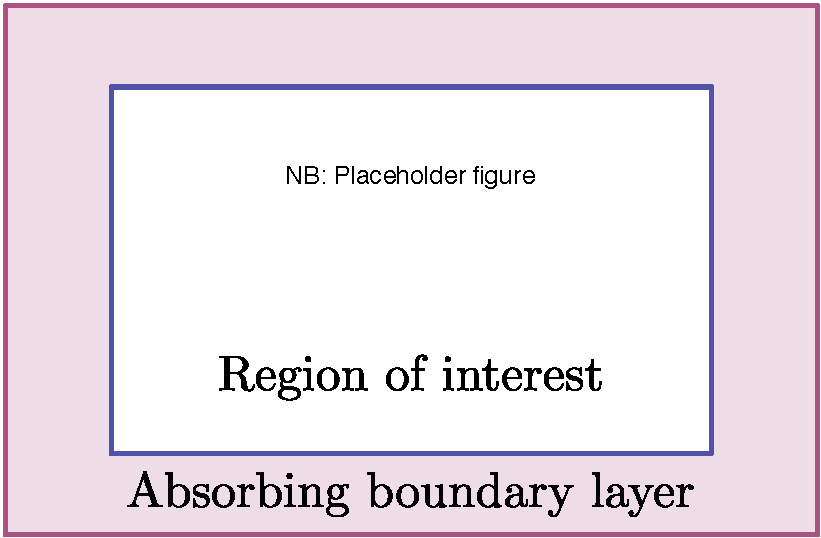
\includegraphics[width=8cm]{RegionOfInterest}
    \caption{A snapshot of the total density from a GP simulation corresponding to the system under discussion in this chapter. It can be observed that the atom laser density is decaying within the absorbing boundary layer. The region of interest and absorbing boundary layer are marked. The region of interest is the entire computational domain except for the absorbing boundary layer. The absorbing boundary layer has a width of $\unit[5]{\micro m}$. \label{Peaks:RegionOfInterest}}
\end{figure}

The rate and distribution with which momentum leaves the region of interest can be determined by considering the equation of motion for the wavenumber density in the region of interest,
\begin{align}
    \frac{\partial }{\partial t}\abs{\widetilde{\psi}_\text{roi}(\vect{k}, t)}^2 &= 2 \Re \left\{ \widetilde{\psi}_\text{roi}^*(\vect{k}, t) \frac{\partial }{\partial t}\widetilde{\psi}_\text{roi}(\vect{k}, t) \right \},
\end{align}
where $\widetilde{\psi}_\text{roi}(\vect{k}, t)$ is the Fourier transform of the restricted wavefunction $\psi_\text{roi}(\vect{x}, t)$, which is defined to be nonzero only within the region of interest. The equation of motion for $\widetilde{\psi}_\text{roi}(\vect{k}, t)$ is
\begin{align}
    \label{Peaks:PsikROIEquationOfMotion}
    \frac{\partial}{\partial t} \widetilde{\psi}_\text{roi}(\vect{k}, t) &= -\frac{i}{\hbar} \mathcal{F}\left[\left(-\frac{\hbar^2 \nabla^2}{2M} + V(\vect{x}) + U \abs{\psi_\text{roi}(\vect{x}, t)}^2\right) \psi_\text{roi}(\vect{x}, t)\right](\vect{k}),
\end{align}
where $\mathcal{F}[f(\vect{x})](\vect{k})$ denotes the Fourier transform of the function $f(\vect{x})$. While the potential and interaction terms in \eqref{Peaks:PsikROIEquationOfMotion} redistribute momentum, it is only due to the kinetic term that momentum will leave the region of interest. To see that this is true, consider a Hamiltonian with no kinetic term. In this case the local phase of the wavefunction will rotate, but the density distribution will remain unchanged. Hence it will be the kinetic term in \eqref{Peaks:PsikROIEquationOfMotion} that will determine the momentum density flux leaving the region of interest.

The Fourier transform of the kinetic term in \eqref{Peaks:PsikROIEquationOfMotion} can be evaluated to give the momentum density flux $\Phi(\vect{k}, t)$ leaving the region of interest in terms of a surface integral over the boundary of the region of interest,
\begin{align}
    \Phi(\vect{k}, t) & = -\frac{\partial }{\partial t}\abs{\widetilde{\psi}_\text{roi}(\vect{k}, t)}^2\bigg|_\text{kinetic}\\
    & = -2 \Re \left\{ \frac{i \hbar}{2 M} \widetilde{\psi}_\text{roi}^*(\vect{k}, t) \frac{1}{(2 \pi)^{\frac{3}{2}}}\oiint e^{-i \vect{k}\cdot \vect{x}} \Big[ \nabla \psi_\text{roi}(\vect{x}, t) + i \vect{k} \psi_\text{roi}(\vect{x}, t)\Big] \cdot d \vect{A} \right\}.
    \label{Peaks:MomentumDensityFluxSurfaceIntegral}
\end{align}
The $\psi_\text{roi}(\vect{x}, t)$ and $\nabla\psi_\text{roi}(\vect{x}, t)$ terms to be evaluated at the boundary in \eqref{Peaks:MomentumDensityFluxSurfaceIntegral} should be understood to be defined by the limit from the interior of the region of interest. While \eqref{Peaks:MomentumDensityFluxSurfaceIntegral} is the most direct way of evaluating $\Phi(\vect{k}, t)$, it is a computationally inefficient method as it requires the calculation of a surface integral for every point $\vect{k}$ at which we wish to evaluate $\Phi(\vect{k}, t)$. 

A more efficient method can be found by instead considering the evolution of the wavenumber density on the entire computational domain. The momentum flux density that left the region of interest enters the absorbing boundary layer through a term like \eqref{Peaks:MomentumDensityFluxSurfaceIntegral}, but leaves at a slightly later time due to the negative imaginary potential. As it is not the temporal dynamics of $\Phi(\vect{k}, t)$ in which we are interested, but just the distribution of momentum that left the region of interest at \emph{any} time, this delay is unimportant. On the entire computational domain, the two kinetic transport terms will cancel leaving the term due to the negative imaginary potential. Assuming that the mean-field interaction energy of the wavefunction reaching the absorbing boundary layer is small compared to its kinetic energy, the momentum flux density leaving the computational domain is given by
\begin{align}
    \label{Peaks:MomentumDensityFlux}
    \Phi(\vect{k}, t)&=\frac{2}{\hbar} \Re \left\{ \widetilde{\psi}^*(\vect{k}, t) \mathcal{F}'\left[ V_I(\vect{x}) \psi(\vect{x}, t)\right](\vect{k}) \right\},
\end{align}
where $\mathcal{F}'$ is the appropriate Fourier-like transform that connects the spatial and spectral representations of the wavefunction $\psi$, and guarantees the artificial boundary conditions are satisfied. Equation \eqref{Peaks:MomentumDensityFlux} is a more efficient method of evaluating $\Phi(\vect{k}, t)$ than \eqref{Peaks:MomentumDensityFluxSurfaceIntegral} as it only requires two Fourier-like transforms to evaluate $\Phi(\vect{k}, t)$ for all $\vect{k}$, instead of one surface integral \emph{for each} $\vect{k}$.

The information provided by either \eqref{Peaks:MomentumDensityFluxSurfaceIntegral} or \eqref{Peaks:MomentumDensityFlux} will only be as good as the absorbing boundary layer. While for a perfect absorbing boundary layer $\int \Phi(\vect{k}, t)\, dt$ would exactly equal the lost momentum density from the region of interest, for an imperfect absorbing boundary layer $\int \Phi(\vect{k}, t)\, dt$ will also include contributions due to any reflection from or transmission through the boundary layer. 

An example calculation of $\Phi(\vect{k}, t)$ for a finite absorbing boundary layer is given in \sectionref{MethodsAppendix:MomentumDensityFluxExampleCalculation}. There it is demonstrated that $\Phi(\vect{k}, t)$ is an accurate method for determining the rate of loss of momentum density from a region of space for the same range of momenta for which the absorbing boundary layer is itself accurate.

\parasep

The simulations described in the remainder of this chapter use the method presented in this section to determine the momentum distribution of atoms that have the left computational domain. This momentum distribution is then propagated classically under gravity to find the corresponding density distribution on the MCP detector below the condensate. This classical propagation was performed by \emph{Mattias Johnsson}. Note that due to the use of cylindrical symmetry, the correct Fourier-like transform for use in \eqref{Peaks:MomentumDensityFlux} is the Hankel (or Bessel) transform~\citep{ArfkenWeber}.

\subsection{Equations of motion}
\label{Peaks:3DEquationsOfMotion}

Having described the calculational techniques that will be used, we now turn to the description of the Gross-Pitaevskii and Truncated Wigner equations that were used to model the experiment. The GP equations that correspond to the master equation \eqref{Peaks:MasterEquation} are
\begin{subequations}
    \label{Peaks:3DGPEquations}
    \begin{align}
        \begin{split}
            i \hbar \frac{\partial }{\partial t}\Psi_1 &= \frac{-\hbar^2 \nabla^2}{2 M} \Psi_1 + \big(V_\text{trap}(\vect{x}) - i V_I(\vect{x})\big)\Psi_1 + \sqrt{2} \hbar \Omega \Psi_0 \\
            & \relphantom{=} + c_0 \sum_j \abs{\Psi_j}^2 \Psi_1 + c_2\left(\abs{\Psi_1}^2 + \abs{\Psi_0}^2 - \abs{\Psi_{-1}}^2 \right) \Psi_1 + c_2 \Psi_{-1}^*\Psi_0^2 \\
            & \relphantom{=} - i \hbar\frac{3}{2}K^\text{(unpol)}_{^{4}\text{He}} \left(2\abs{\Psi_{-1}}^2 \Psi_1 - \Psi_{-1}^* \Psi_0^2\right),
        \end{split}\\
        \begin{split}
            i \hbar \frac{\partial }{\partial t}\Psi_0 &= \frac{-\hbar^2 \nabla^2}{2 M} \Psi_0 + \big(\hbar \Delta - i V_I(\vect{x}) \big)\Psi_0 + \sqrt{2} \hbar \Omega \Psi_1 + \sqrt{2}\hbar\Omega \Psi_{-1} \\
            & \relphantom{=} + c_0 \sum_j \abs{\Psi_j}^2 \Psi_0 + c_2\left(\abs{\Psi_1}^2 + \abs{\Psi_{-1}}^2 \right) \Psi_0 + 2 c_2 \Psi_{0}^*\Psi_1\Psi_{-1} \\
            & \relphantom{=} - i \hbar\frac{3}{2}K^\text{(unpol)}_{^{4}\text{He}} \left(\abs{\Psi_{0}}^2 \Psi_0 - 2\Psi_{0}^* \Psi_1\Psi_{-1}\right),
        \end{split}\\
        \begin{split}
            i \hbar \frac{\partial }{\partial t}\Psi_{-1} &= \frac{-\hbar^2 \nabla^2}{2 M} \Psi_{-1} + \big(-V_\text{trap}(\vect{x}) + 2 \hbar \Delta - i V_I(\vect{x})\big)\Psi_{-1} + \sqrt{2} \hbar \Omega \Psi_0 \\
            & \relphantom{=} + c_0 \sum_j \abs{\Psi_j}^2 \Psi_{-1} + c_2\left(-\abs{\Psi_1}^2 + \abs{\Psi_0}^2 + \abs{\Psi_{-1}}^2 \right) \Psi_{-1} + c_2 \Psi_{1}^*\Psi_0^2 \\
            & \relphantom{=} - i \hbar\frac{3}{2}K^\text{(unpol)}_{^{4}\text{He}} \left(2\abs{\Psi_{1}}^2 \Psi_{-1} - \Psi_{1}^* \Psi_0^2\right),
        \end{split}
    \end{align}
\end{subequations}
where $\displaystyle V_\text{trap}(\vect{x}) = \frac{1}{2} M \left(\omega_r^2 r^2 + \omega_z^2 z^2 \right)$ is the trapping potential, $\hbar \Delta$ is the detuning in energy of the resonant outcoupling surface from the centre of the condensate, $c_0 = (g_0 + 2 g_2)/3$, $c_2 = (g_2 - g_0)/3$, where $g_S = 4 \pi \hbar^2 a_S/M$ is the nonlinear interaction strength, and $a_S$ is the $s$-wave scattering length for the total hyperfine spin $S$ channel (refer to \sectionref{BackgroundTheory:AtomicScattering}). A derivation of the Penning ionisation terms in \eqref{Peaks:3DGPEquations} is given in \sectionref{PenningIonisationAppendix:GP}.

The Truncated Wigner equations corresponding to the master equation \eqref{Peaks:MasterEquation} are very similar to \eqref{Peaks:3DGPEquations} but with some additional terms. In Stratonovich form, the equations of motion for the stochastic wavefunctions are approximately
% See MolecularScattering.nb for the derivation of the Penning ionisation terms
\begin{align}
    \label{Peaks:3DTWEquations}
    \begin{split}
        \left. i \hbar \,d\vect{\Psi}\right|_\text{TW} &\approx \left. i \hbar \frac{\partial }{\partial t}\vect{\Psi}\right|_\text{GP} dt - \left(2 c_0 + c_2 \right)\frac{1}{\Delta V}\vect{\Psi}\, dt\\
        &\relphantom{\approx} + i\sqrt{ \hbar V_I(\vect{x})} \,d\vect{W}(\vect{x}) + i \hbar\sqrt{3 \Kunpol}
        \begin{pmatrix}
            \Psi_{-1}^*\\
            \Psi_0^*\\
            \Psi_1^*
        \end{pmatrix} dW_p(\vect{x}),
    \end{split}
\end{align}
where $\Delta V$ is the computational grid's volume element (for irregularly spaced grids such as those that used for cylindrically symmetric problems, $\Delta V$ is the local Gaussian quadrature weight~\citep{Ronen:2006}), $\vect{\Psi} = \left(\Psi_1, \Psi_0, \Psi_{-1} \right)^T$ and $d \vect{W}(\vect{x}) = \big(dW_1(\vect{x}), dW_0(\vect{x}), dW_{-1}(\vect{x})\big)^T$ and $dW_p(\vect{x})$ are the complex Gaussian noises satisfying
\begin{align}
    \overline{dW_i(\vect{x})\, dW_j(\vect{x}')} &= 0 \\
    \overline{dW_i(\vect{x})\, dW_j^*(\vect{x}')} &= \frac{1}{\Delta V}\delta_{ij}\delta_{\vect{x},\vect{x}'}\,dt, \label{Peaks:ComplexNoiseExpectationValue}
\end{align}
where $\overline{(\cdots)}$ denotes the expectation value taken with respect to the noises. The usual spatial Dirac delta function in \eqref{Peaks:ComplexNoiseExpectationValue} has been replaced by a Kronecker delta function scaled by the inverse volume element due to the discretisation of the problem onto a computational grid.

The origin of the additional terms in \eqref{Peaks:3DTWEquations} can be understood qualitatively in terms of the `virtual' particles added to the initial state required in Truncated Wigner (see \sectionref{BackgroundTheory:StochasticPhaseSpaceMethods}). The $\Delta V^{-1}$ term corrects for the contribution to \emph{s}-wave scattering due to the virtual particles. The $d \vect{W}$ term corrects for the loss of virtual particles due to the absorbing boundary layer and the $dW_p$ term does similarly for the virtual particles lost due to Penning ionisation.

The approximation made in obtaining \eqref{Peaks:3DTWEquations} was to neglect $\Delta V^{-1}$ compared to the field occupations $\abs{\Psi_1}^2$, $\abs{\Psi_0}^2$, $\abs{\Psi_{-1}}^2$ in the Penning ionisation noise term. This is justified for large occupations where Penning ionisation will be significant. The approximation cannot be made where the density is low, but at these locations the Penning ionisation process itself can be neglected as the associated rate constant will have decreased proportionally with the density. A derivation of the Penning ionisation noise term in \eqref{Peaks:3DTWEquations} is given in \sectionref{PenningIonisationAppendix:TW}.

\parasep

One might like to imagine that the task is essentially complete once a set of equations has been derived that describes a system. Unfortunately, technical considerations often limit which problems are and are not feasible to solve. In this case, although the GP equations given in \eqref{Peaks:3DGPEquations} can be solved in a couple of days on a supercomputer, \eqref{Peaks:3DTWEquations} represents a much more challenging problem. Not only do these equations need to be solved a large number of times for different initial conditions, but algorithms for solving stochastic differential equations are limited to a lower order\footnote{There is no known bound on the order of algorithms for solving stochastic (partial) differential equations, however algorithms for strong solutions require the evaluation of an exponentially increasing number of higher-order noise integrals with increasing order of the algorithm~\citep{Burrage:1997}. For weak solutions (what is required here) the highest-order algorithms known that only require the evaluation of $O(N)$ noise integrals have global order $O(\Delta t^2)$~\citep{Rosler:2007,Rosler:2009}, where $N$ is the number of Gaussian noises required (as the noises are spatially-dependent, $N$ is proportional to the size of the computational grid and hence the evaluation of $O(N^2)$ or more noise integrals is infeasible).} than those that can be used for deterministic differential equations hence significantly smaller time steps are required for solving stochastic differential equations. This problem is mainly due to the $\Psi_{-1}$ state which, due to the antitrapping potential, has a kinetic energy $\sim 40$ times larger than the $\Psi_{0}$ atoms at the edge of the computational domain $\unit[60]{\micro m}$ away from the centre of the condensate in the radial direction. The computational domain cannot be restricted to be tighter due to the requirement that the mean-field energy of the $\Psi_{0}$ atoms be negligible compared to their kinetic energy for the absorbing boundary layer to be effective. While it is for these practical reasons that we must neglect the $\Psi_{-1}$ state, we are physically justified in doing so by the same arguments given at the start of \sectionref{Peaks:PerturbativeApproach}. 

In the next sections the behaviour of the atom laser in the cases of outcoupling from the centre of the condensate (resonant outcoupling) and outcoupling from a detuned surface where the atom laser flux is maximised are considered.

\subsection{Verification of semianalytical model}

As a verification of the results of \sectionref{Peaks:PerturbativeApproach} we consider outcoupling from the centre of the condensate ($\Delta = 0$). This is the case that corresponds most closely with that of the homogenous condensate considered in \sectionref{Peaks:PerturbativeApproach} because the shape of the outcoupling surfaces (see \figureref{Peaks:OutcouplingSurfaces}) restricts outcoupling to the centre of the condensate where the density is a local maximum; there the condensate is locally homogeneous.

\begin{figure}
    \centering
    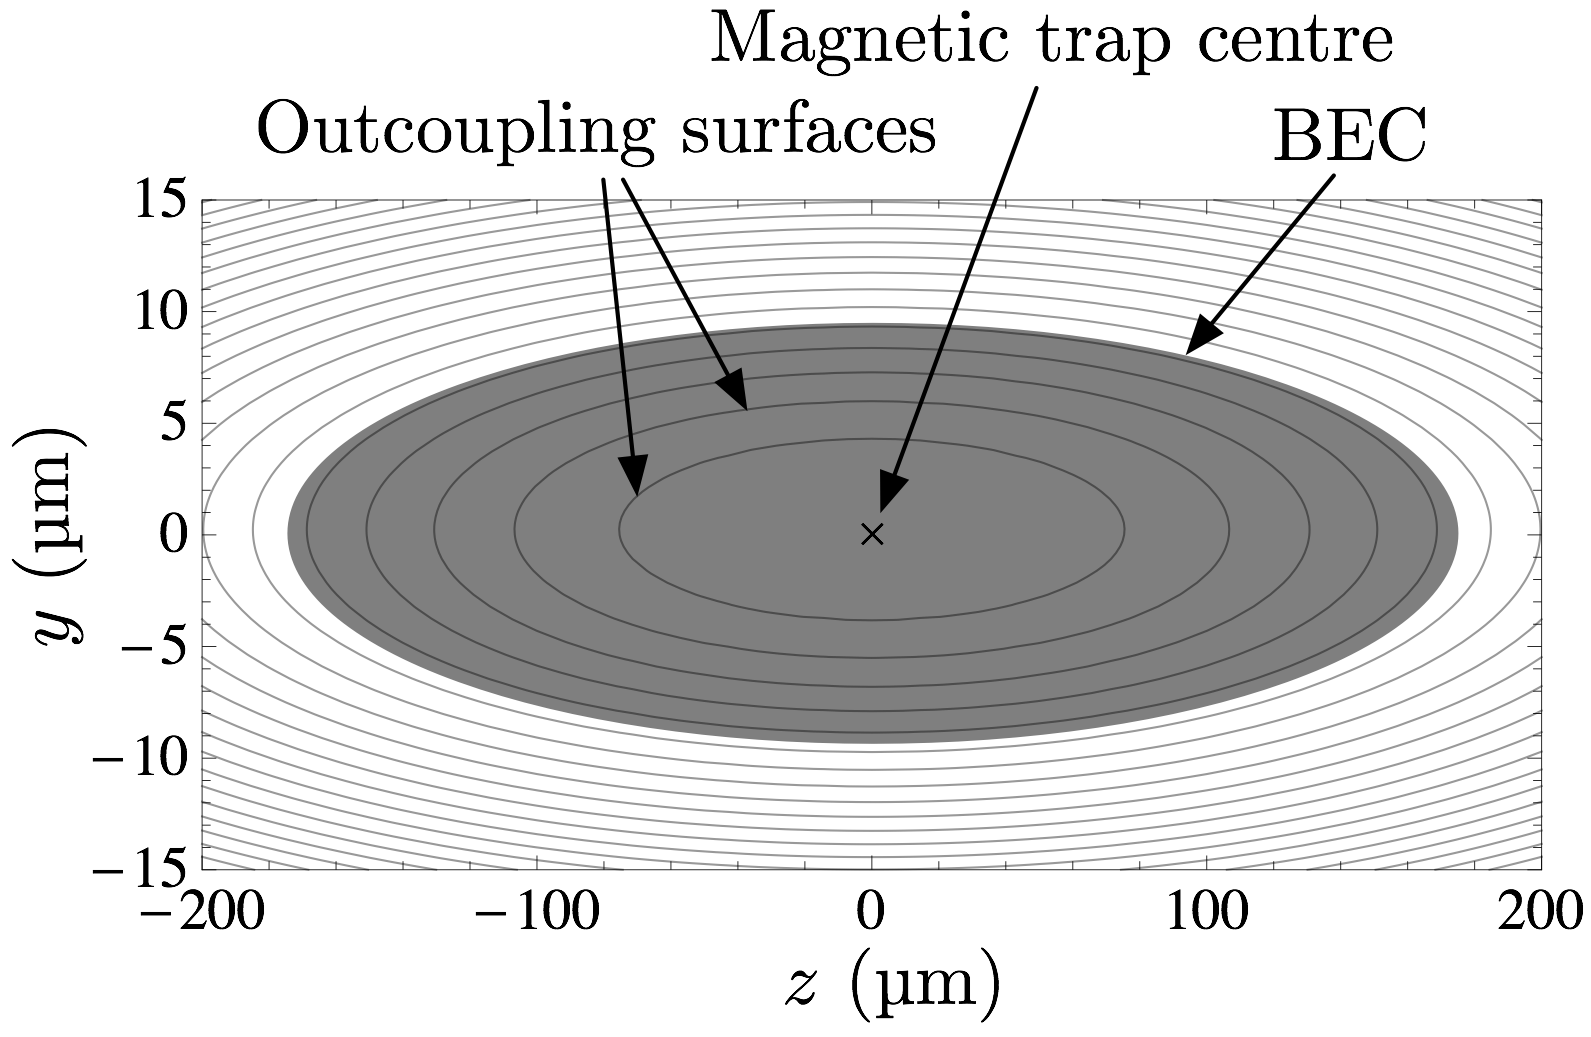
\includegraphics[width=8cm]{OutcouplingSurfaces}
    \caption{Outcoupling surfaces of the He* condensate under consideration in this chapter.  The small gravitational sag of $y_\text{sag} = \unit[0.2]{\micro m}$ means that the centre of the trap and the centre of the condensate almost exactly coincide.  Hence the outcoupling surfaces are approximately centred on the centre of the condensate.  The contours pictured are equally-spaced in energy.  The aspect ratio of this figure is not 1:1 for reasons of clarity; the condensate is significantly more elongated than pictured. \label{Peaks:OutcouplingSurfaces}}
\end{figure}

\begin{figure}
    \centering
    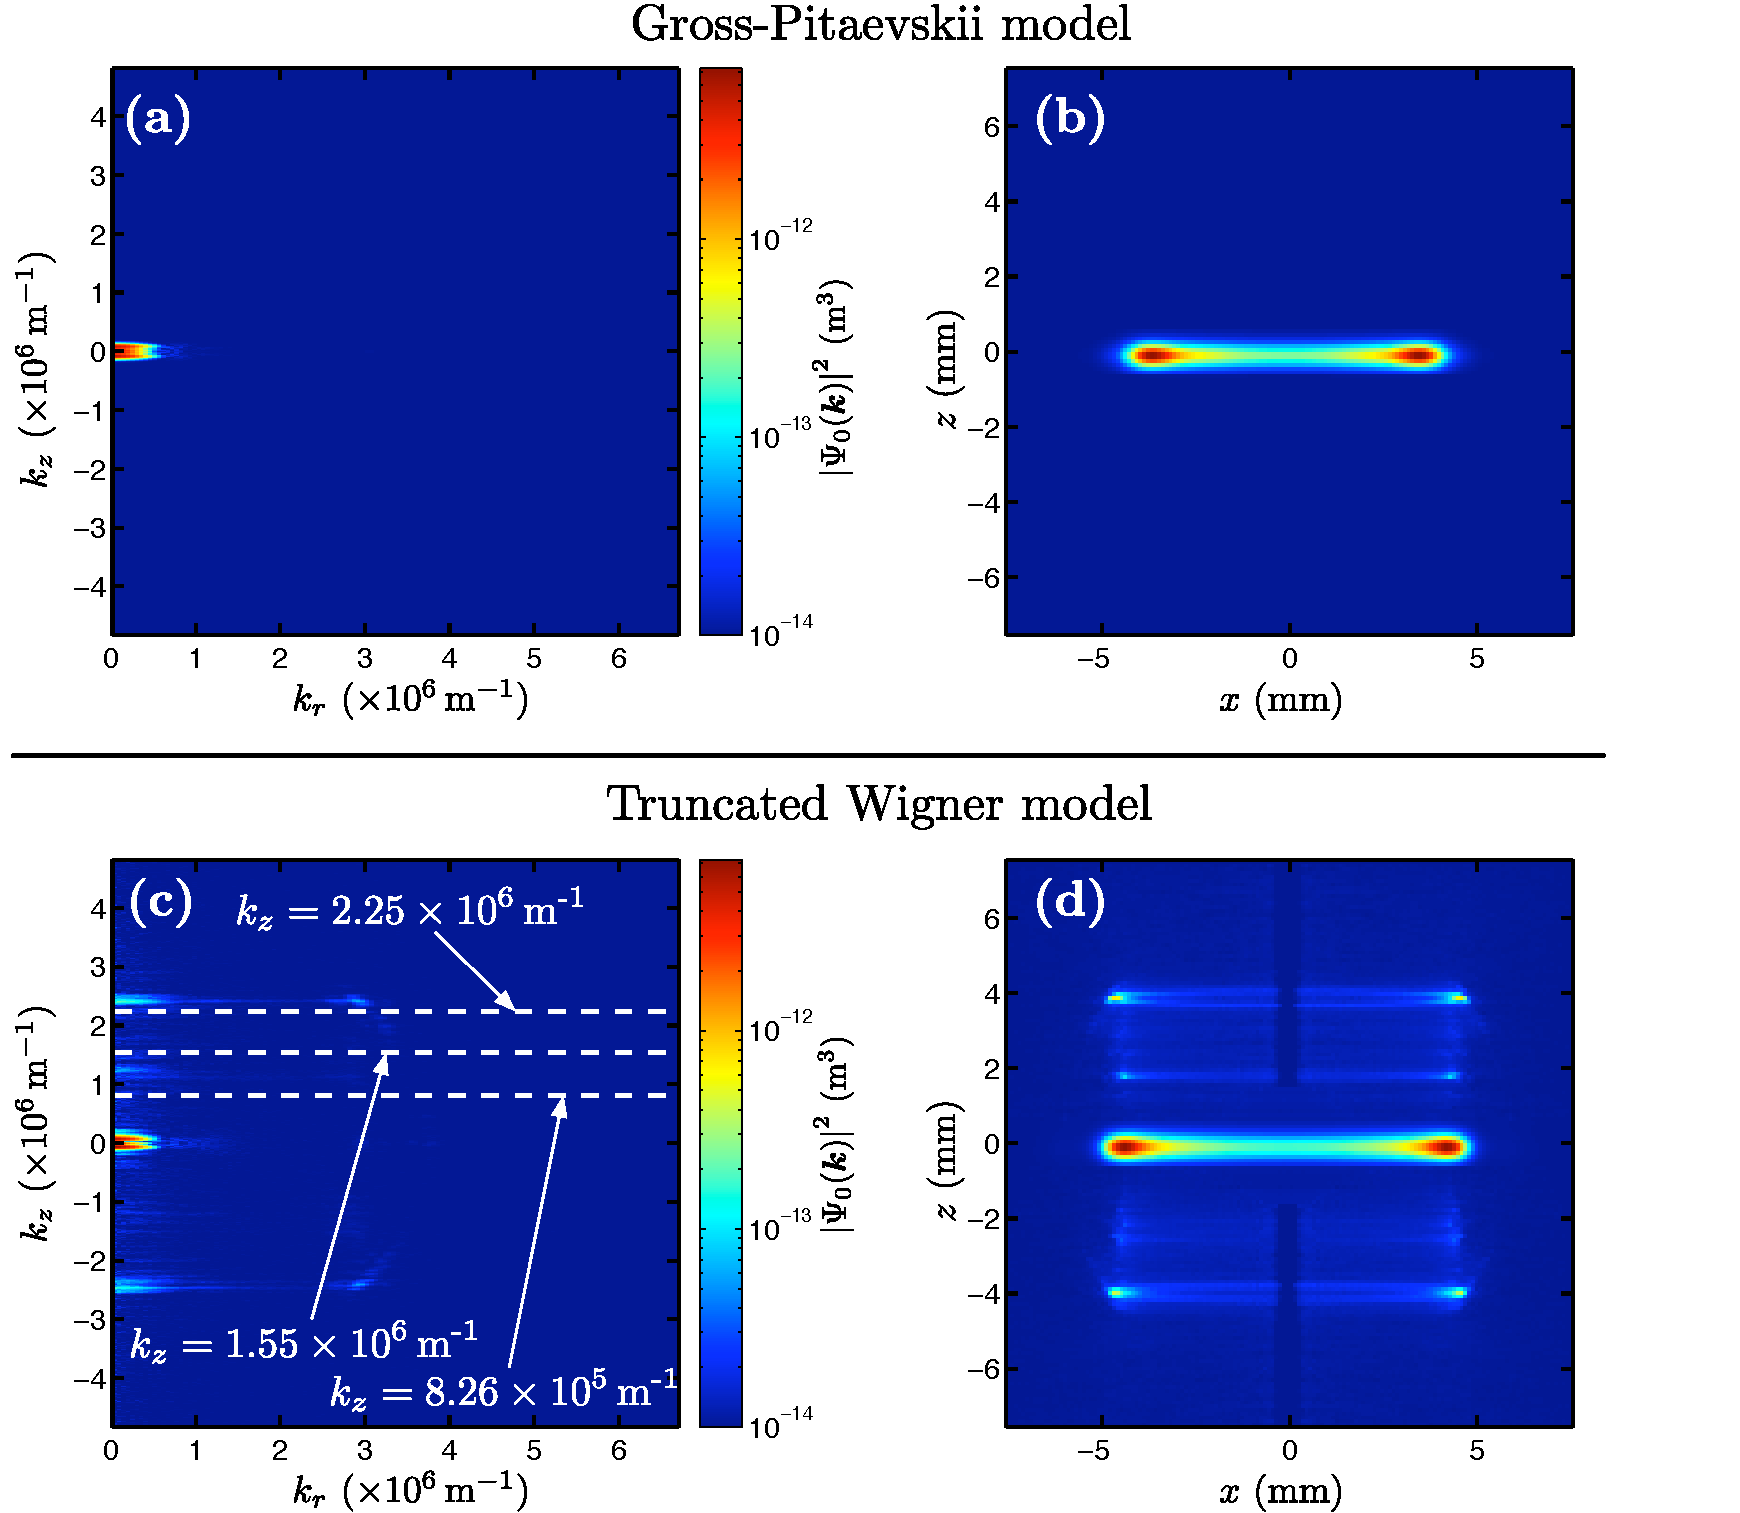
\includegraphics[trim=0 0 52 0,width=14cm]{ResonantOutcouplingNoPI}
    \caption{Simulation results for outcoupling from the centre of the condensate without Penning ionisation. Left figures (a) and (c) plot the momentum density of the untrapped state at $t=\unit[2]{ms}$ as a function of the radial ($k_r$) and axial ($k_z$) wavenumbers. Right figures (b) and (d) plot the normalised density profiles that would be observed on the MCP detector $\unit[4]{cm}$ below the condensate due to outcoupling from the condensate for $t=\unit[6]{ms}$. The upper figures (a) and (b) plot the results of a GP model where the $m_F=-1$ state is assumed negligible, lower figures (e) and (f) correspond to a Truncated Wigner simulation for the same system averaged over $N_\text{realisations} = 4$. The wavenumbers of the three fastest-growing instabilities predicted by the perturbation analysis performed in \sectionref{Peaks:PerturbativeApproach} are marked in (c). The weak axis is in the vertical direction in all figures.\label{Peaks:TheoryZeroDetuningNoPIResults}}
\end{figure}

The results of the GP and TW simulations for the case of resonant outcoupling but in the absence of Penning ionisation are presented in \figureref{Peaks:TheoryZeroDetuningNoPIResults}. The atom laser momentum density for the GP and TW simulations are displayed in \figureref{Peaks:TheoryZeroDetuningNoPIResults}(a) and (c). The primary contribution to the momentum density is around $(k_r \approx 0, k_z \approx 0)$ due to Rabi coupling to the Bose-Einstein condensate. Due to the high aspect ratio of the condensate, these atoms are strongly accelerated along the radial direction and hence move to the right in \figureref{Peaks:TheoryZeroDetuningNoPIResults}(a) and (c). At times earlier than $t=\unit[2]{ms}$ which is pictured in \figureref{Peaks:TheoryZeroDetuningNoPIResults}(a) and (c) there is an additional peak at $(k_r \approx \unit[2.8 \times 10^6]{m}^{-1}, k_z \approx 0)$ due to the main atom laser after it has accelerated out of the condensate. This peak disappears around $t=\unit[1.8]{ms}$ due to the formation of a bound state (see~\citep{Robins:2005uq}) causing the atom laser to shutdown.

The primary feature of the MCP detector profiles depicted in \figureref{Peaks:TheoryZeroDetuningNoPIResults}(b) and (d) is the atom laser profile in the middle of both images. The double-peak structure of the atom laser profile was discussed earlier in \sectionref{BackgroundTheory:TransverseProfile}. Briefly, the broad structure is due to the strong acceleration of the atom laser out of the condensate in the radial direction leading to a ring in momentum space (the peak at $(k_r \approx \unit[2.8 \times10^6]{m}^{-1}, k_z \approx 0)$ discussed above). Due to the expansion of the atom laser during as it falls, the measured density on the MCP detector corresponds to the vertically integrated momentum distribution as depicted in \figureref{Peaks:Schematic}. The vertical integration of the ring-shaped momentum distribution directly leads to the double-peak structure in the main atom laser profile in \figureref{Peaks:TheoryZeroDetuningNoPIResults}(b) and (d). Neither the fine structure nor the `shadow' of the BEC in the atom laser profile discussed in \sectionref{BackgroundTheory:TransverseProfile} are observed in \figureref{Peaks:TheoryZeroDetuningNoPIResults} due to the use of a purely classical method to propagate the momentum density from the edge of the computational region to the detector. However these details are not of interest in this chapter.

The spontaneously-seeded dynamical instabilities predicted in \sectionref{Peaks:PerturbativeApproach} are observed in the results of the Truncated Wigner model shown in \figureref{Peaks:TheoryZeroDetuningNoPIResults}, but absent from the results of the Gross-Pitaevskii model due to its neglect of spontaneously-seeded processes. Moreover, the dynamical instability with the largest growth rate illustrated in \figureref{Peaks:CondensateEigenvalues} at $k=\unit[2.25\times 10^6]{m}^{-1}$ is in good agreement with the highest growth rate instability in \figureref{Peaks:TheoryZeroDetuningNoPIResults}(c) observed at $(k_r \approx 0,\, k_z \approx \pm\unit[2.4\times 10^6]{m}^{-1})$. As discussed above this instability is outcoupled from the condensate and then accelerates radially outwards (to the right in \figureref{Peaks:TheoryZeroDetuningNoPIResults}(c)) to produce rings in momentum space. These rings appear as the double-peaked structures on the MCP detector away from the main atom laser profile in \figureref{Peaks:TheoryZeroDetuningNoPIResults}(d). The formation process of the instabilities is illustrated in \figureref{Peaks:ResonantOutcouplingProcess} and a comparison is made to the results of the GP model in which these instabilities do not occur\footnote{Although not pictured, the instabilities \emph{are} observed in the GP model, appearing just after $t=\unit[6]{ms}$. The appearance of these instabilities however is not for physical reasons, instead it is caused by the amplification of numerical noise in the simulation. A higher-precision GP simulation would show the instabilities appearing at a later time.}.

\begin{sidewaysfigure}
    \centering
    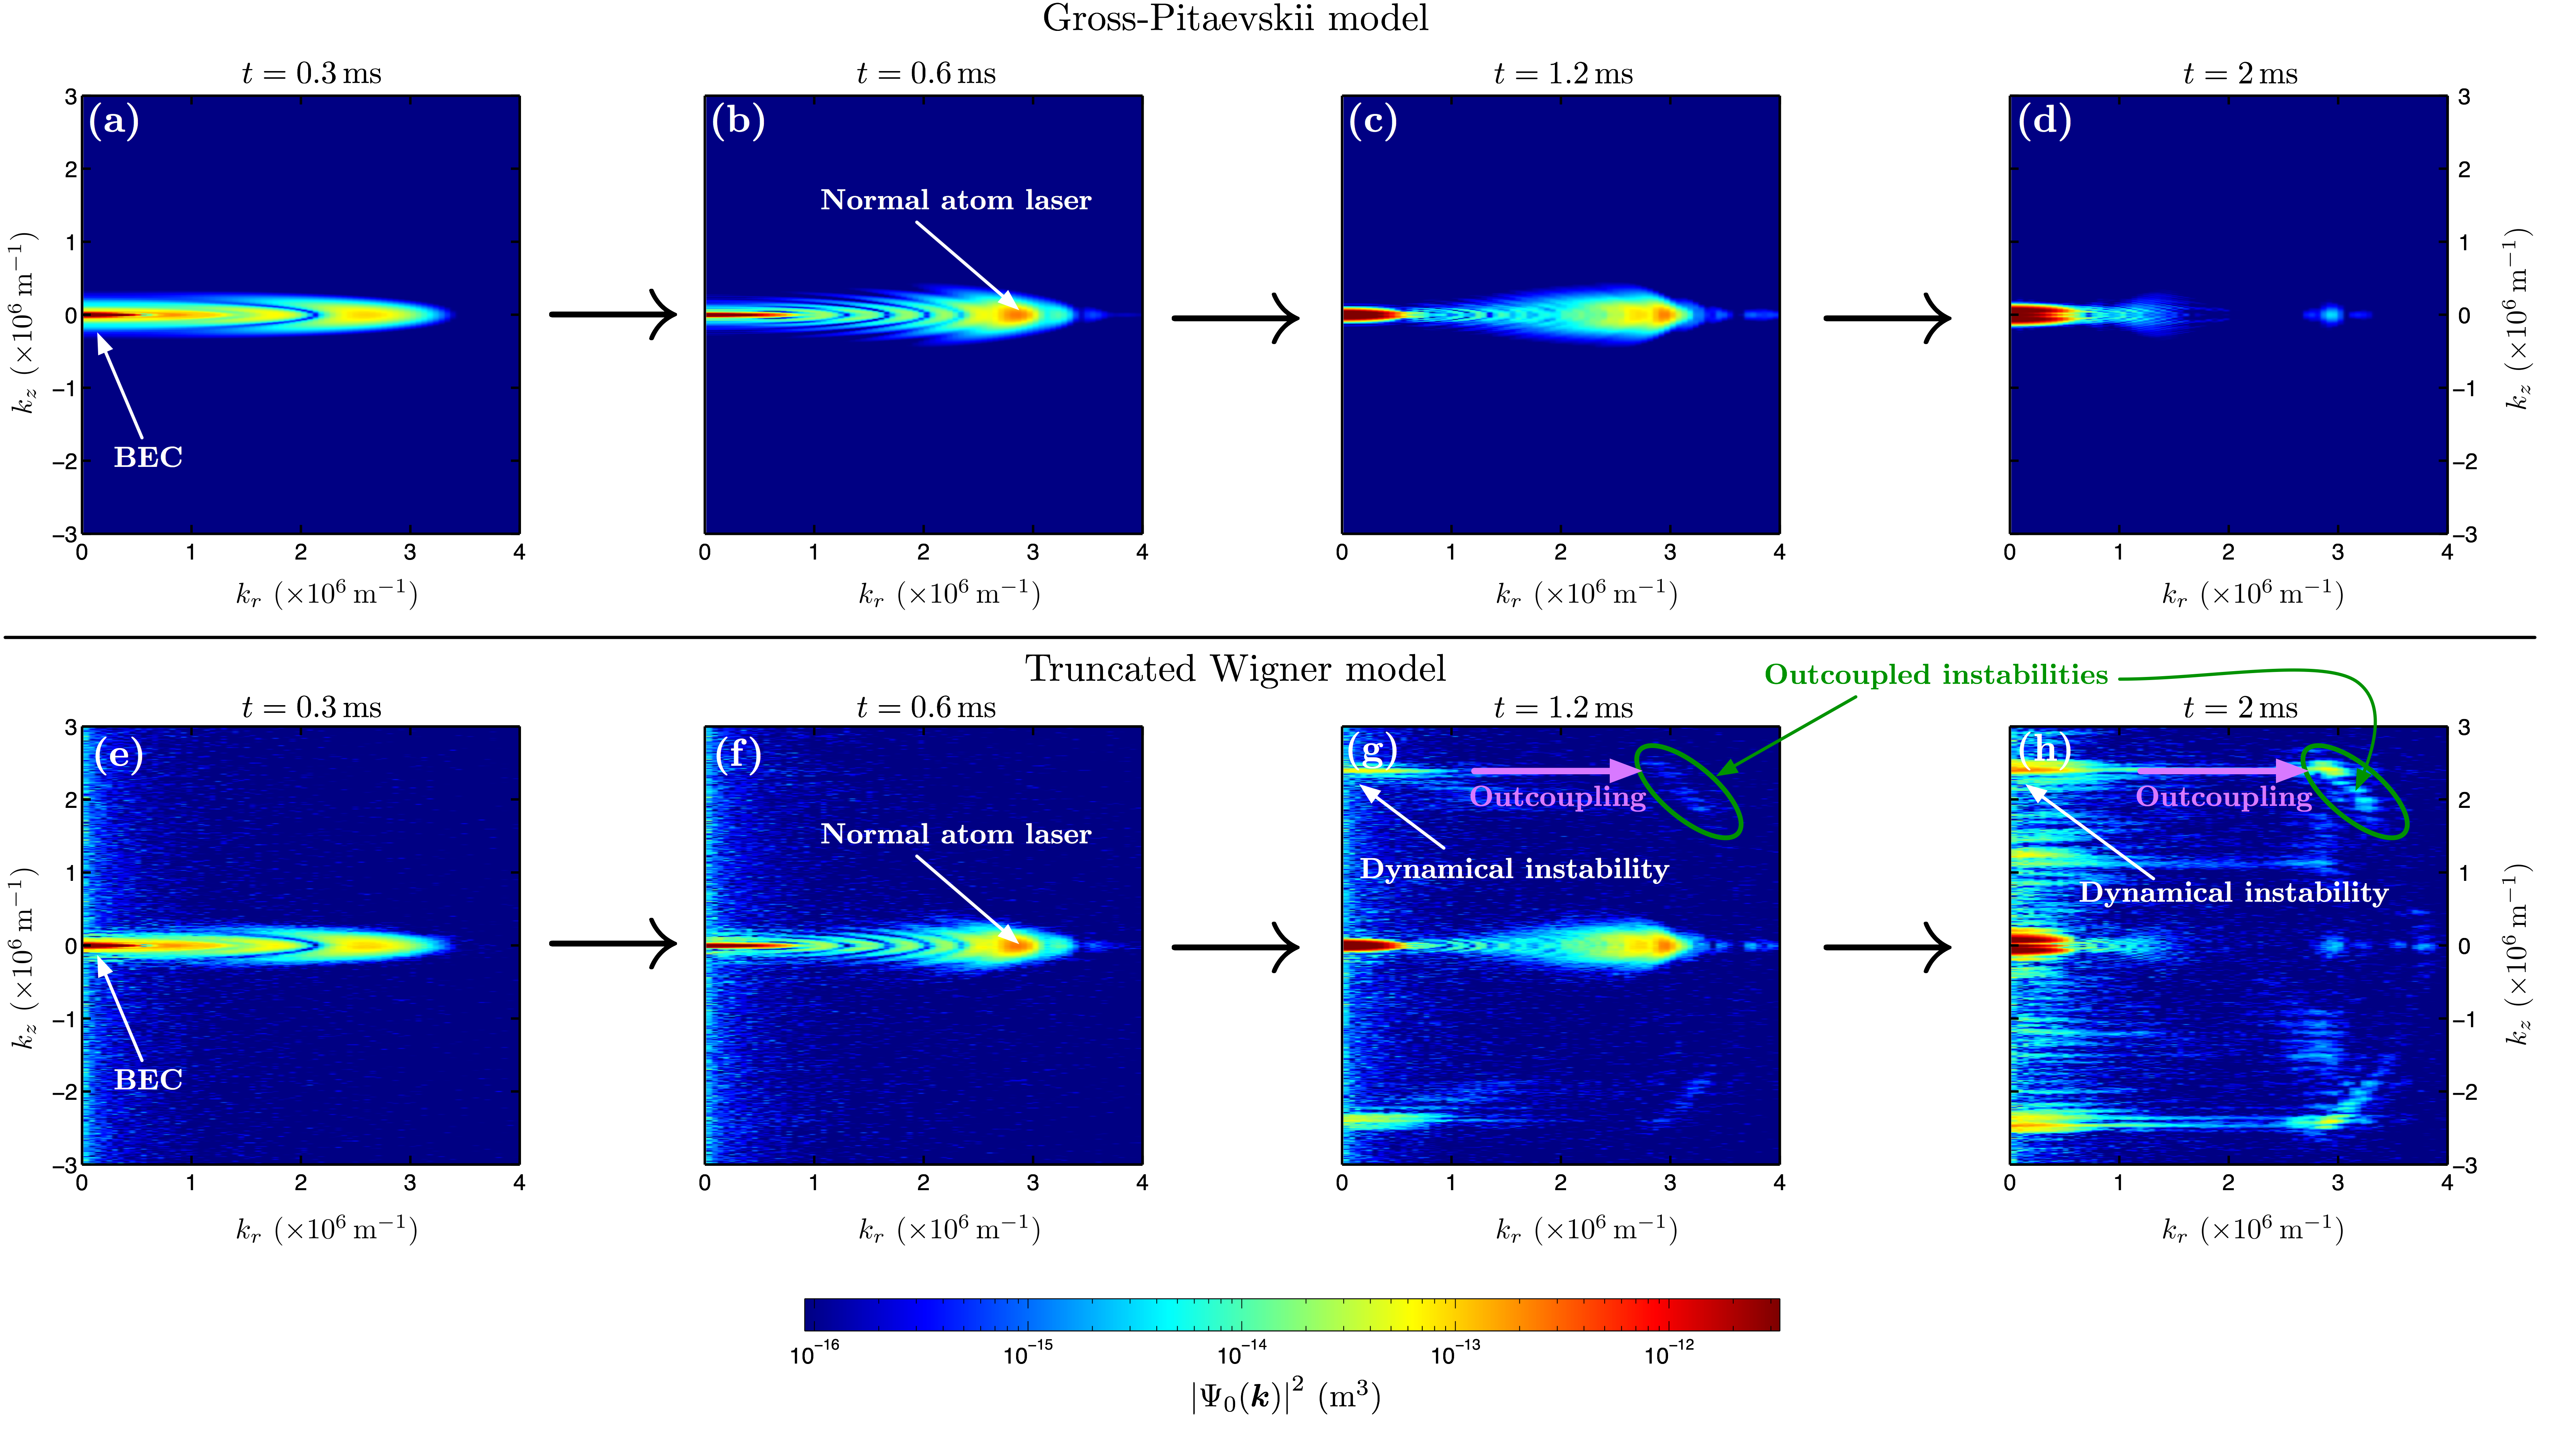
\includegraphics[width=22cm]{ResonantOutcouplingProcess}
    \caption{Simulation results for outcoupling from the centre of the condensate without Penning ionisation illustrating the formation of the normal atom laser profile and the dynamical instabilities. Upper figures (a)--(d) are the results of a two level Gross-Pitaevskii model, and lower figures (e)--(h) are the results of a two level Truncated Wigner model. The upper and lower rows respectively correspond to the upper and lower rows of \figureref{Peaks:TheoryZeroDetuningNoPIResults}. The columns from left to right show the evolution of the momentum density $\abs{\Psi_0(\vect{k})}^2$ of the untrapped state at times: \unit[0.3]{ms}, \unit[0.6]{ms}, \unit[1.2]{ms}, and \unit[2]{ms}.
    This figure illustrates that the instabilities are spontaneously seeded and that modes between the main atom laser profile and the instabilities are not significantly populated until after the instability has formed. The marked `Normal atom laser' part of the momentum density distribution is the component that corresponds to the MCP atom laser profile shown in \figureref{Peaks:TheoryZeroDetuningNoPIResults}(b).  Note that the vacuum noise in (e)--(h) is not uniform because the initial vacuum noise is proportional to the inverse volume element, which due to the assumed cylindrical symmetry $\displaystyle \Delta V_{\vect{k}}^{-1} \propto k_r^{-1}$.\label{Peaks:ResonantOutcouplingProcess}}
\end{sidewaysfigure}

As discussed in \sectionref{Peaks:DynamicalInstabilitiesDiscussion} the dynamical instabilities observed in \figureref{Peaks:TheoryZeroDetuningNoPIResults} will be entangled when they are produced, however the entangled modes are superpositions of the $\Psi_1$ and $\Psi_0$ states with opposite momenta. It will not be feasible to directly detect this entanglement as the outcoupling process will significantly complicate the spatial structure of the entangled modes. Although only the $\Psi_0$ state can leave the magnetic trap, the $\Psi_1$ component of the entangled mode is likely to be outcoupled faster than the time it would take to perform half an oscillation and reverse the sign of its axial momentum ($\sim \unit[9]{ms}$). Consequently number difference squeezing between the opposite momentum components of the entangled modes should be robust enough to survive outcoupling. It cannot be proven due to the small number of realisations calculated, however it is expected that there should exist number difference squeezing between the number of atoms above and below the main atom laser beam in \figureref{Peaks:TheoryZeroDetuningNoPIResults}. The main atom laser beam must be excluded as it is produced due to entirely classical means and hence would not be have number difference squeezing.

Although not pictured, the results of a GP model including all three atomic levels $\Psi_1$, $\Psi_0$ and $\Psi_{-1}$ are of the same form as the results presented in \figureref{Peaks:TheoryZeroDetuningNoPIResults}(a) and (b).




% \subsubsection{In the presence of Penning ionisation}
% Including Penning ionisation in the GP and TW simulations complicates the comparison of the results with the perturbative model presented in \sectionref{Peaks:PerturbativeApproach} as Penning ionisation will interfere with the growth processes and possibly suppress them. The results of GP and TW simulations for the case of resonant outcoupling and in the presence of Penning ionisation are presented in \figureref{Peaks:TheoryZeroDetuningPIResults}. It is noted that the spontaneously seeded structures observed in \figureref{Peaks:TheoryZeroDetuningNoPIResults} blah blah blah.
% 
% \begin{figure}
%     \centering
%     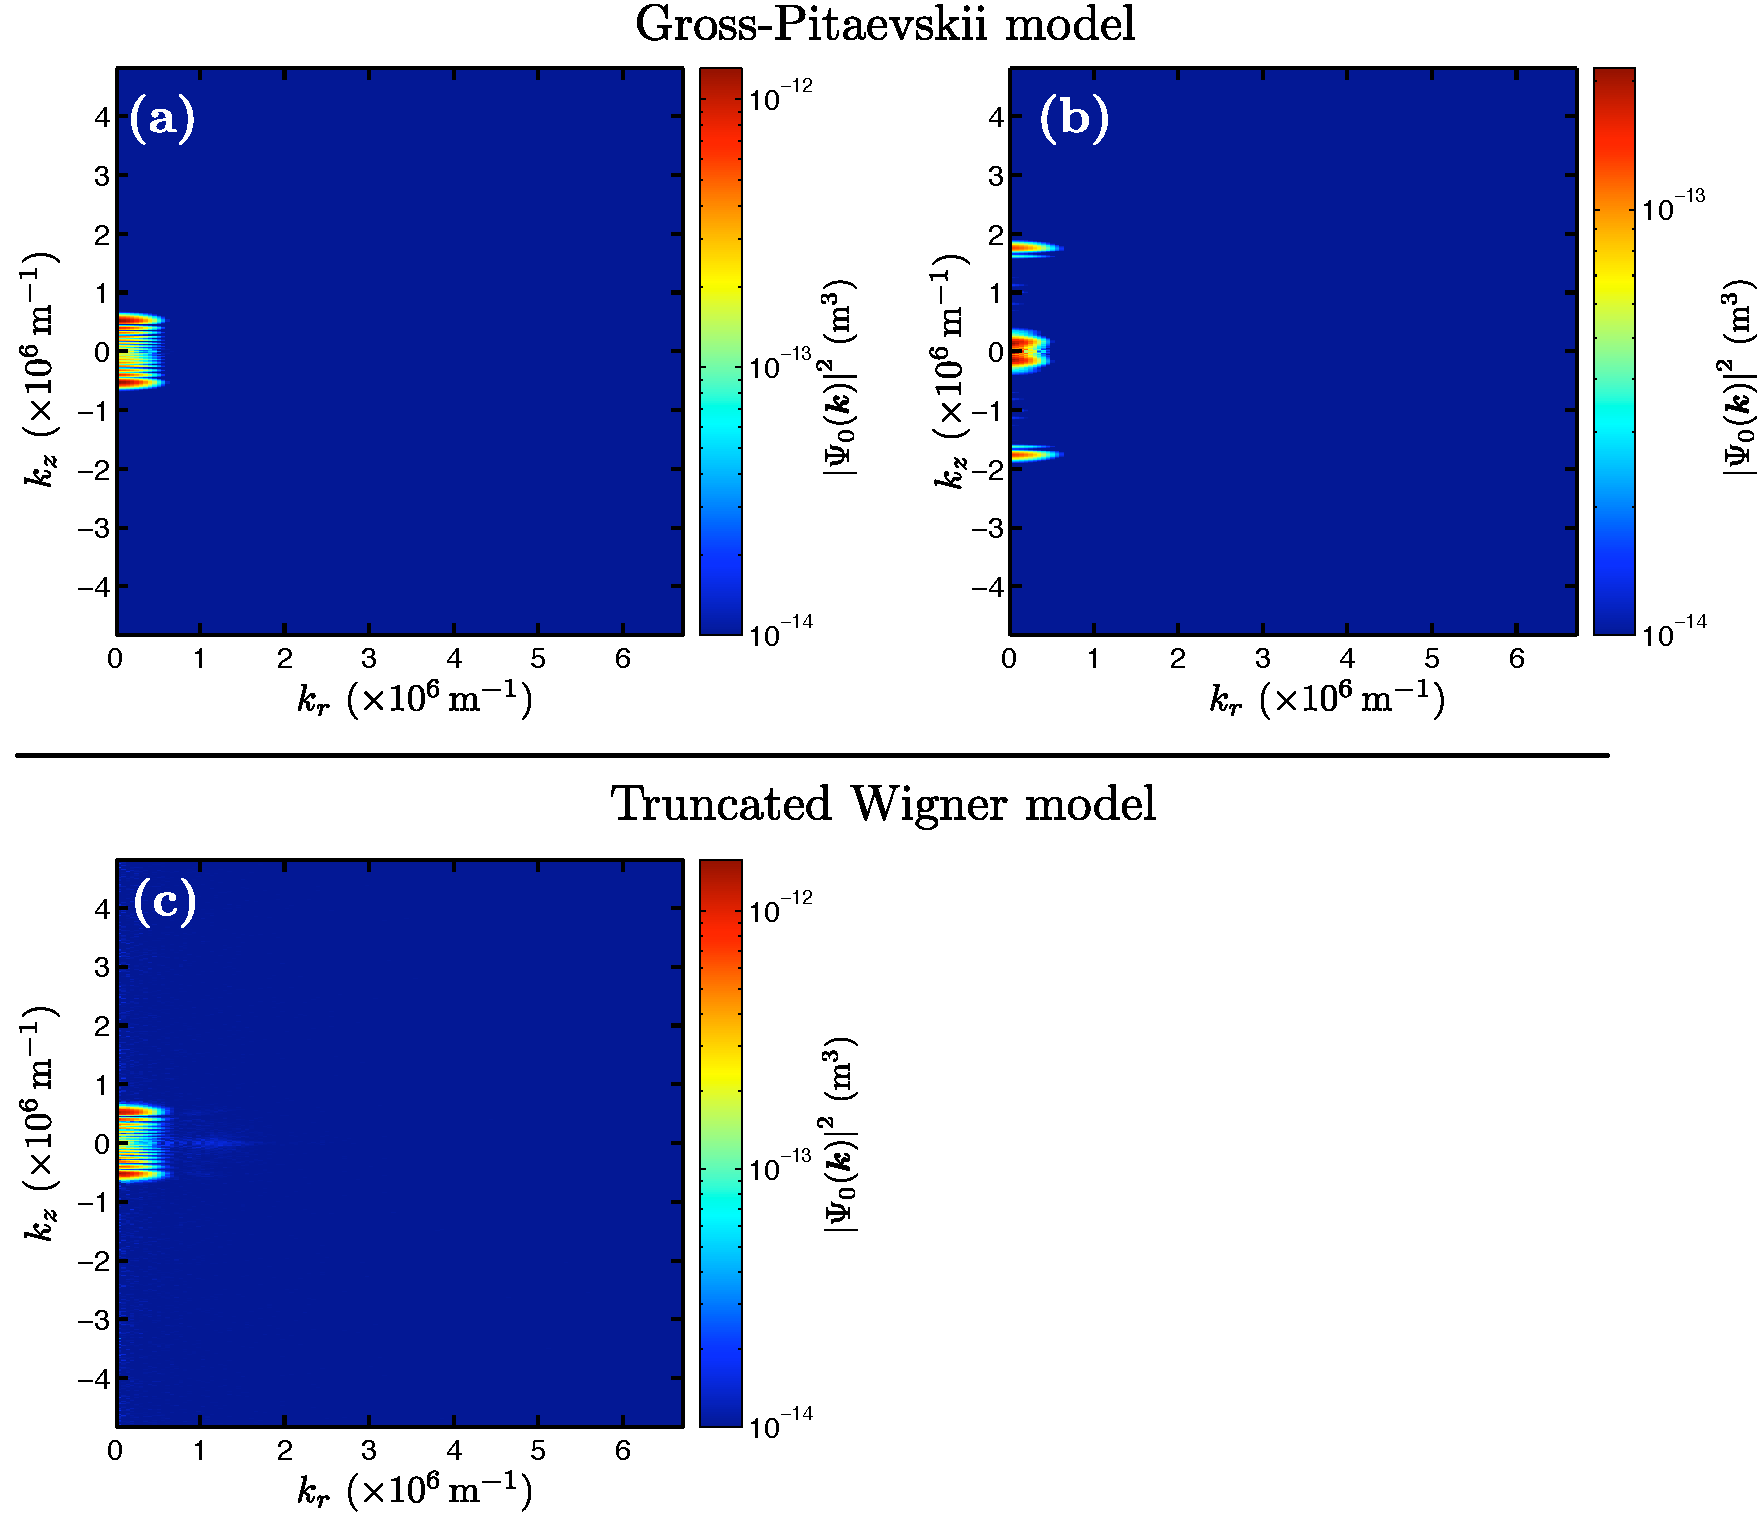
\includegraphics[width=14cm]{ResonantOutcouplingPI}
%     \caption{\label{Peaks:TheoryZeroDetuningPIResults} Simulation results for outcoupling from the centre of the condensate with Penning ionisation.}
% \end{figure}



% 
% The case in which Penning ionisation
% 
% \hrule
% 
% Next step: Penning ionisation.
% 
% As expected, the spontaneously-seeded dynamical instabilities predicted in \sectionref{Peaks:PerturbativeApproach} are not observed in the GP simulations where spontaneous scattering does not occur. Moreover, two of the dynamical instabilities predicted in \sectionref{Peaks:PerturbativeApproach} are observed in the results of the TW simulation with the third indistinguishable from the vacuum fluctuations due to the small number of realisations used. Although Penning ionisation was not considered in \sectionref{Peaks:PerturbativeApproach}, it can be seen from the results presented in \figureref{Peaks:TheoryZeroDetuningNoPIResults} that the instabilities have not been suppressed by Penning ionisation.
% 
% As the instabilities in \figureref{Peaks:TheoryZeroDetuningNoPIResults}(c) are outcoupled it can be observed that they accelerate along the radial direction forming momentum cones such as those pictured in \figureref{Peaks:Schematic}. When these momentum cones fall onto the detector they are vertically integrated to produce the well-defined peak-like structures in \figureref{Peaks:TheoryZeroDetuningNoPIResults}(d). Although these instabilities are entangled upon formation, it is unlikely that any useful entanglement will survive the outcoupling process as it is only the $\Psi_0$ and $\Psi_{-1}$ states that can escape the condensate. Despite this, it is likely that there will be number-difference squeezing between opposite points on the momentum cones as the characteristic time for the outcoupling process $\sim \unit[3]{ms}$ is much less than the time for an atom to undergo an oscillation in the weak trapping direction of $\sim \unit[18]{ms}$. Consequently, it is unlikely that the $\Psi_1$ component of the instability will remain in the condensate long enough for its momentum in the weak trapping dimension to change significantly. This number-difference squeezing between opposite points on the momentum-cones would be observed as a number difference squeezing between the structures on the opposite sides of the main atom laser profile in \figureref{Peaks:TheoryZeroDetuningNoPIResults}(d). Unfortunately, due to the computational difficulty of the problem, it is not at present possible to theoretically verify the claim of number-difference squeezing due to the large number of realisations that would be required for any results to have statistical significance.
% 
% To take into account the estimated expansion due to mean-field repulsion in the beam itself, we use an approximate method where we convolve the detector profiles with a Gaussian of width $\unit[200]{\micro m}$.
% 


\subsection{Comparison of Theory and Experiment}

In the previous section the behaviour of the atom laser when outcoupling from the centre of the condensate was considered.  In this limit it was found that the results of full 3D simulations were in good agreement with the semianalytical model presented in \sectionref{Peaks:PerturbativeApproach}.  The features in \figureref{Peaks:TheoryZeroDetuningNoPIResults}(d) and \figureref{Peaks:ExperimentalResults}(b) should therefore be interpreted as the result of the dynamical instabilities discussed in \sectionref{Peaks:PerturbativeApproach}. 

While the theoretical results presented in \figureref{Peaks:TheoryZeroDetuningNoPIResults}(d) show some similarity to the experimental results [\figureref{Peaks:ExperimentalResults}(b)], there are qualitative differences.  As will be shown in this section, these qualitative differences are due to the difference in detunings used in these two results.  While the theoretical results were for the case of outcoupling from the centre of the condensate, the experimental results were for the case of detuned outcoupling.  Resonant outcoupling can be understood in terms of the semianalytical model presented in \sectionref{Peaks:PerturbativeApproach} as the multimode behaviour of the full condensate only affects the dynamics weakly because the net force on atoms outcoupled from the centre of the trap is zero.  The direct application of the semianalytical model for detuned outcoupling is complicated by the multimode dynamics which are now evolve on a comparable timescale to the instabilities due to the nonzero net force on outcoupled atoms.  Although the model cannot be directly applied in this case it is reasonable to expect similar behaviour.  This expectation must be checked numerically.

The experimental results presented in \figureref{Peaks:ExperimentalResults} were not obtained by outcoupling from the centre of the condensate but instead a nonzero detuning of $\Delta = 2 \pi \times \unit[6.5]{kHz}$ was used, which is a significant fraction of the chemical potential $\mu/\hbar = 2\pi \times \unit[18]{kHz}$. This detuning was for the practical reason that when outcoupling near the centre of the condensate, the atom laser flux \emph{decreases} as the outcoupling surface moves towards the centre of the condensate (for the same rf outcoupling power). This behaviour can be explained using a simple model in which the  outcoupled atom laser flux is proportional to the surface area of the outcoupling surface times the average density over that surface. Outcoupling from the centre of the condensate will therefore lead to a small atom laser flux due to the small surface area (see \figureref{Peaks:OutcouplingSurfaces}). Detuning will cause the atom laser flux to increase as the surface area increases before decreasing again as the condensate density drops off towards the edge of the condensate. This behaviour is shown in \figureref{Peaks:DetuningCurve}. The experimental results presented in \figureref{Peaks:ExperimentalResults} were for the detuning which maximises the atom laser flux, which can be seen from \figureref{Peaks:DetuningCurve} to be $\Delta = 2\pi \times \unit[6.5]{kHz}$.

\begin{figure}
    \centering
    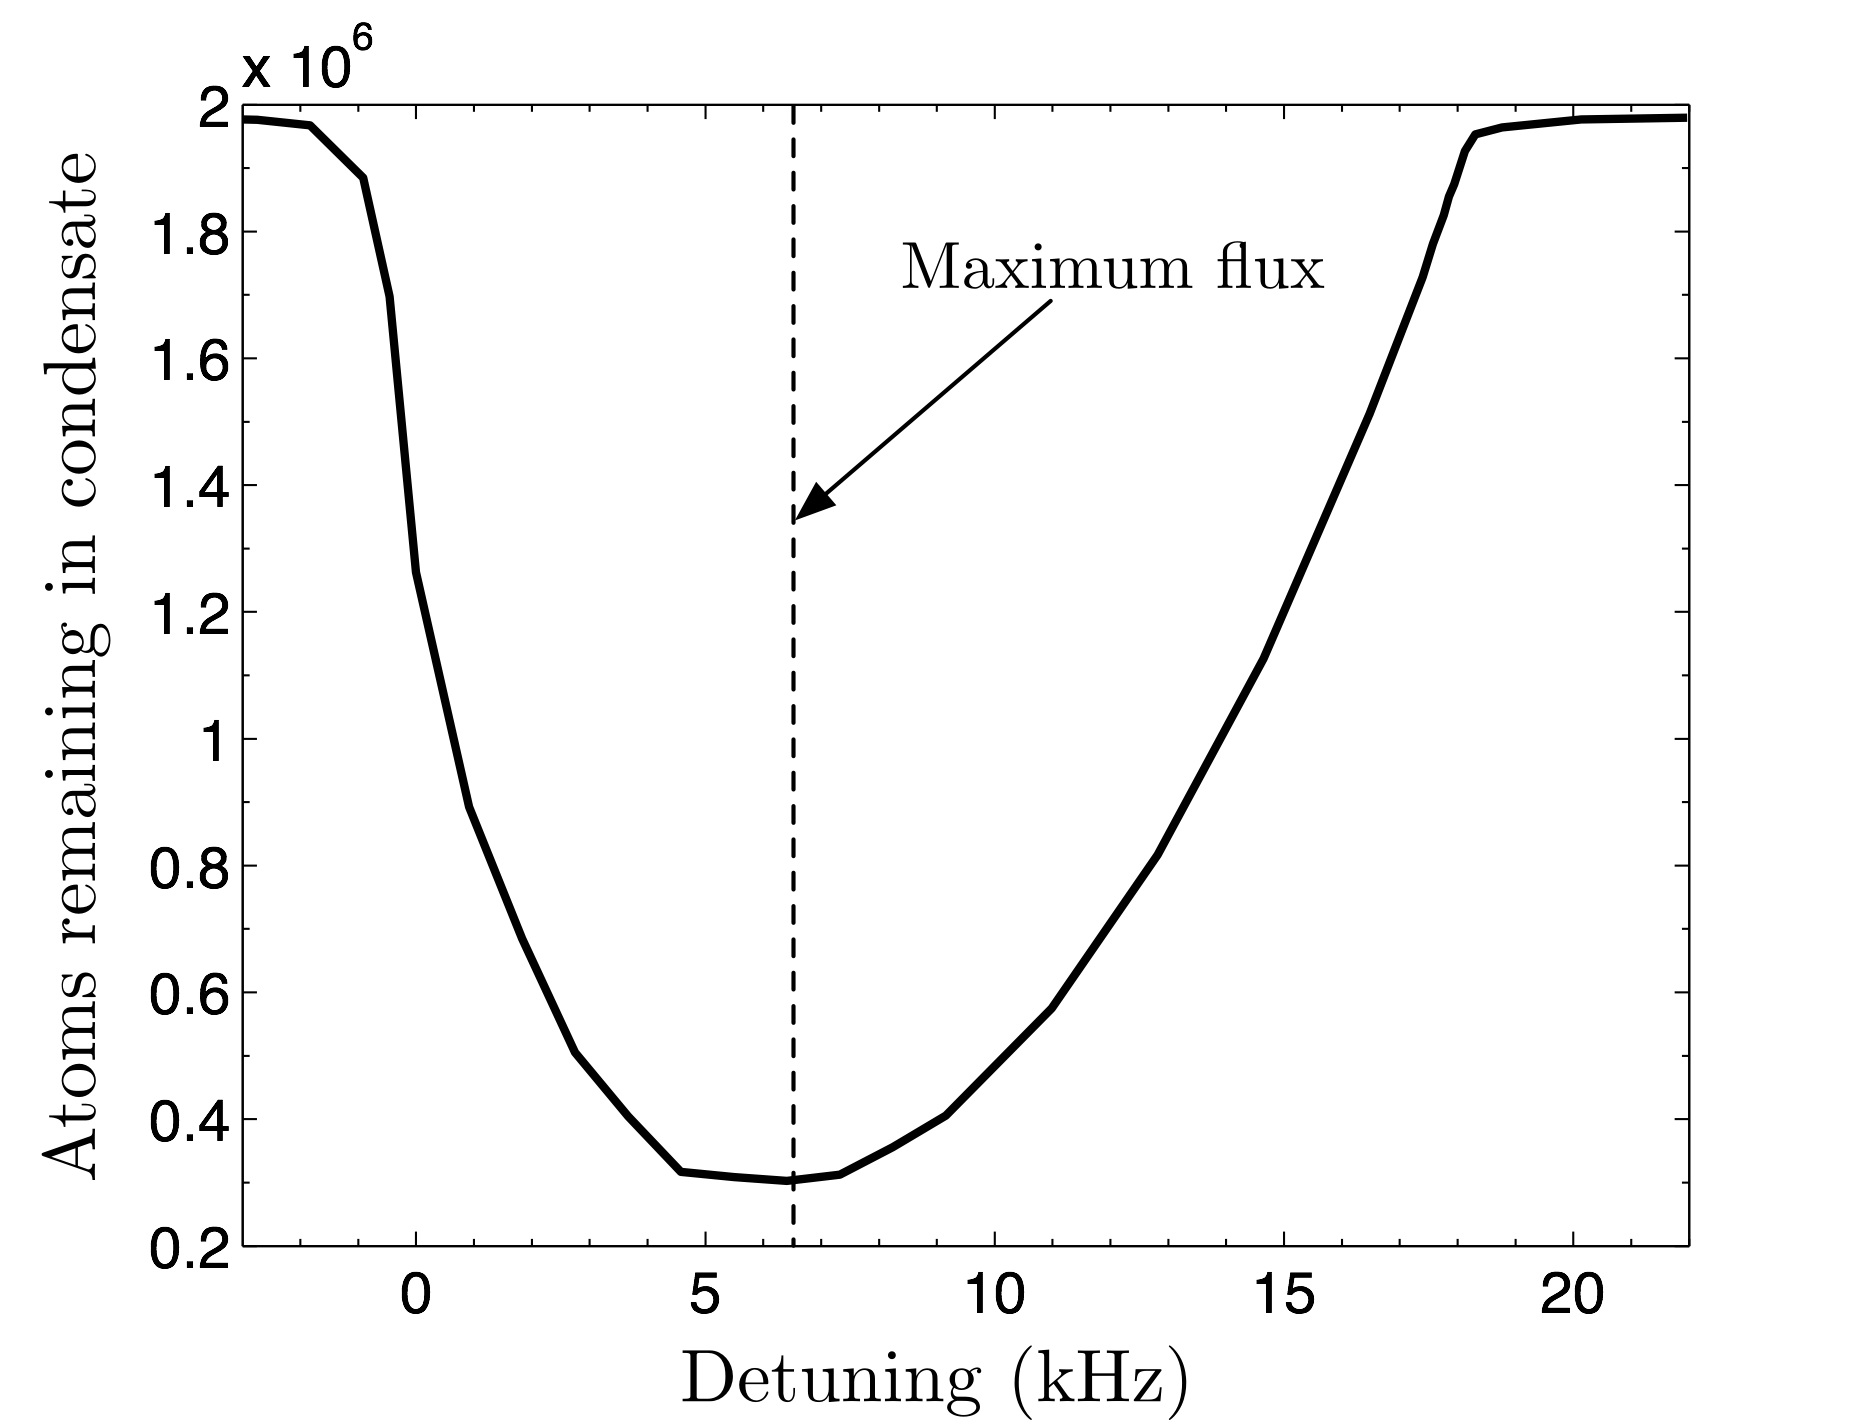
\includegraphics[width=8cm]{DetuningCurve}
    \caption{Theoretical calculation of the number of atoms remaining in the condensate after $\unit[10]{ms}$ of outcoupling at a Rabi frequency of $\Omega = \unit[210]{Hz}$ as a function of the detuning of the rf outcoupling from the centre of the condensate. The results shown are obtained from simulations of the 3D GP equations for the condensate under consideration. \label{Peaks:DetuningCurve}}
\end{figure}

\begin{figure}
    \centering
    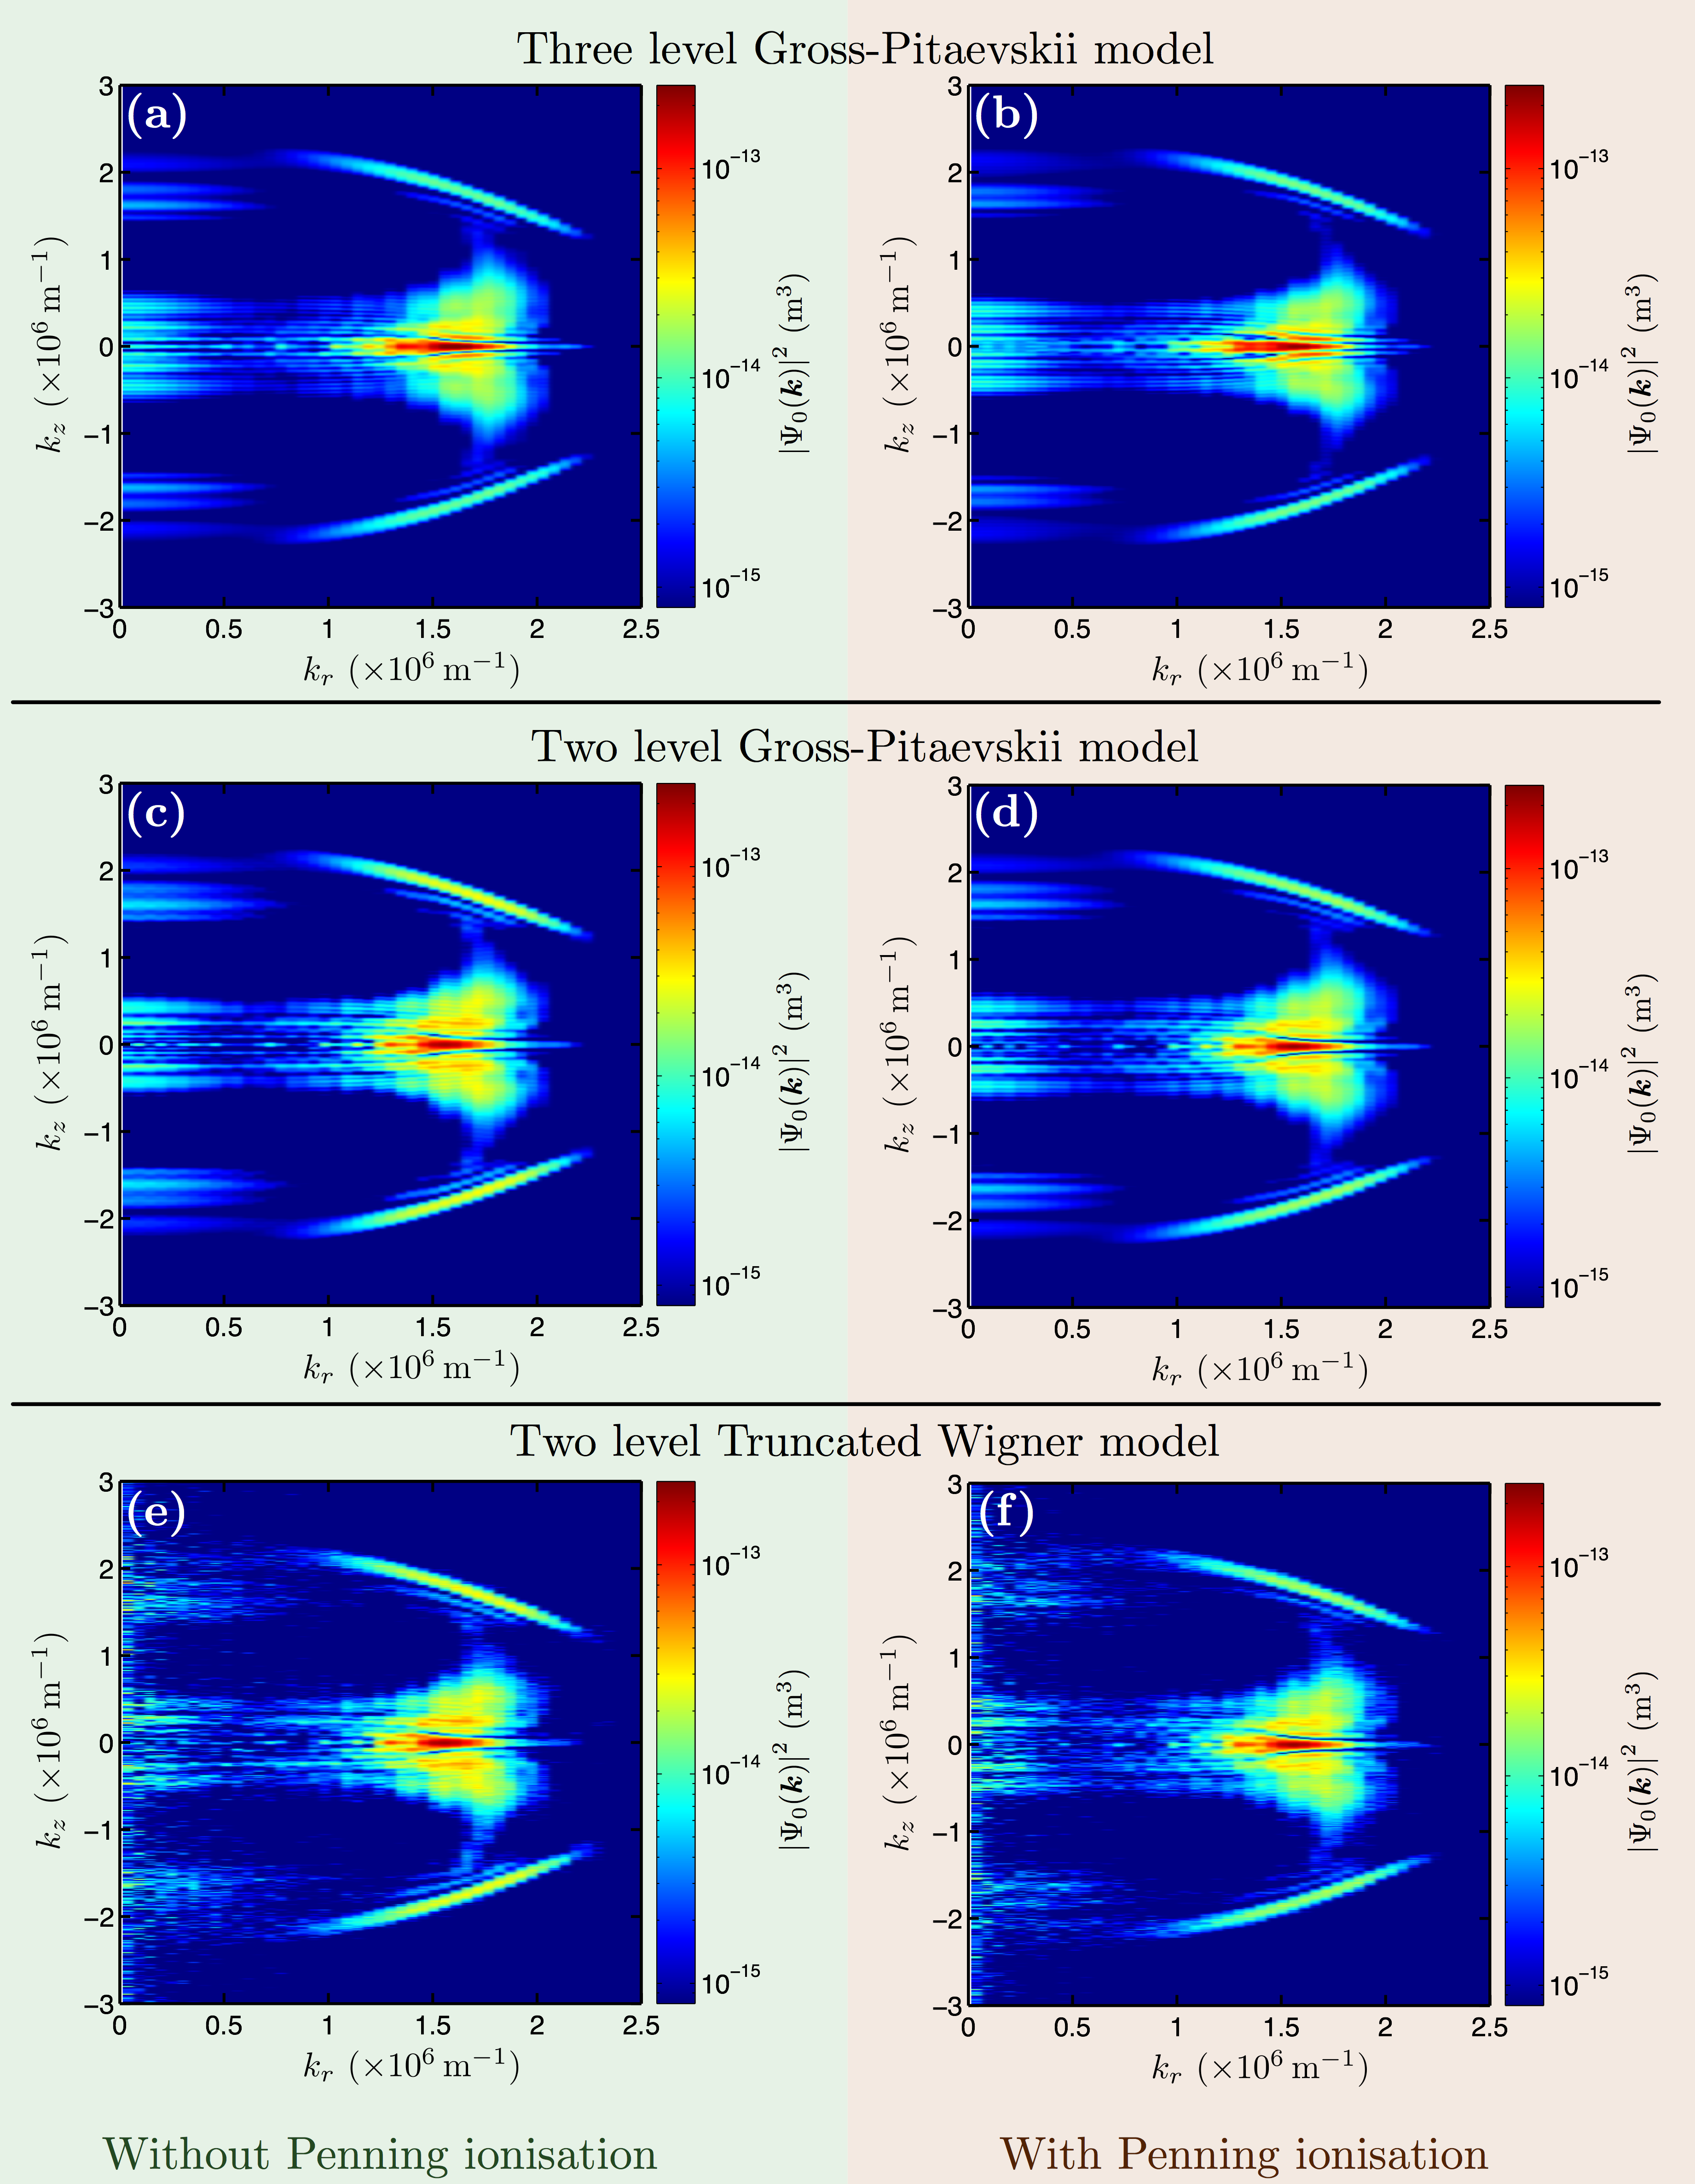
\includegraphics[width=14cm]{DetunedOutcouplingModelComparison}
    \caption{Simulation results for outcoupling with a detuning of $\Delta = 2\pi \times \unit[6.5]{kHz}$ from the centre of the condensate, with and without including the effects of Penning ionisation (right and left columns respectively). The upper figures (a) and (b) plot the results of a GP model including all $m_F$ atomic levels. Middle figures (c) and (d) plot the results of a reduced GP model where the $m_F=-1$ is assumed negligible, lower figures (e) and (f) correspond to a Truncated Wigner simulation for the same system with $N_\text{realisations} = 4$. The negligible difference between the figures in the left and right columns indicate that Penning ionisation has a negligible impact in the simulations depicted.\label{Peaks:TheoryMaxFluxDetuningResults}}
\end{figure}

The results of 2-level TW and 2- and 3-level GP simulations of the experiment for a detuning of $\Delta = 2\pi \times \unit[6.5]{kHz}$ are shown in \figureref{Peaks:TheoryMaxFluxDetuningResults}. As discussed at the end of \sectionref{Peaks:3DEquationsOfMotion}, a 3-level TW model is too computationally demanding to simulate, although the similarity of the results of the three models presented in \figureref{Peaks:TheoryMaxFluxDetuningResults} suggests that the results of such a simulation would differ negligibly from those presented.

The results pictured in \figureref{Peaks:TheoryMaxFluxDetuningResults} are of the momentum density $\abs{\Psi_0(\vect{k})}^2$ of the $m_F=0$ untrapped state at $t=\unit[5.1]{ms}$.  A comparison of the results of simulations with and without Penning ionisation are also shown (right and left columns respectively), which demonstrate that the features depicted are not suppressed by Penning ionisation.  As expected, the features of the momentum density profiles in \figureref{Peaks:TheoryMaxFluxDetuningResults} have a similar form to those in \figureref{Peaks:TheoryZeroDetuningNoPIResults}(c).  An important difference is that for detuned outcoupling, the features at large $\abs{k_z}$ appear in both the TW and GP models indicating that these structures are \emph{not} spontaneously seeded.  \figureref{Peaks:DetunedPeaksFormationProcess} illustrates the formation process of these structures demonstrating that they are produced by a stimulated scattering process from the condensate that sweeps in momentum from $k_z=0$ towards the final state pictured in \figureref{Peaks:TheoryMaxFluxDetuningResults}. 

\begin{sidewaysfigure}
    \centering
    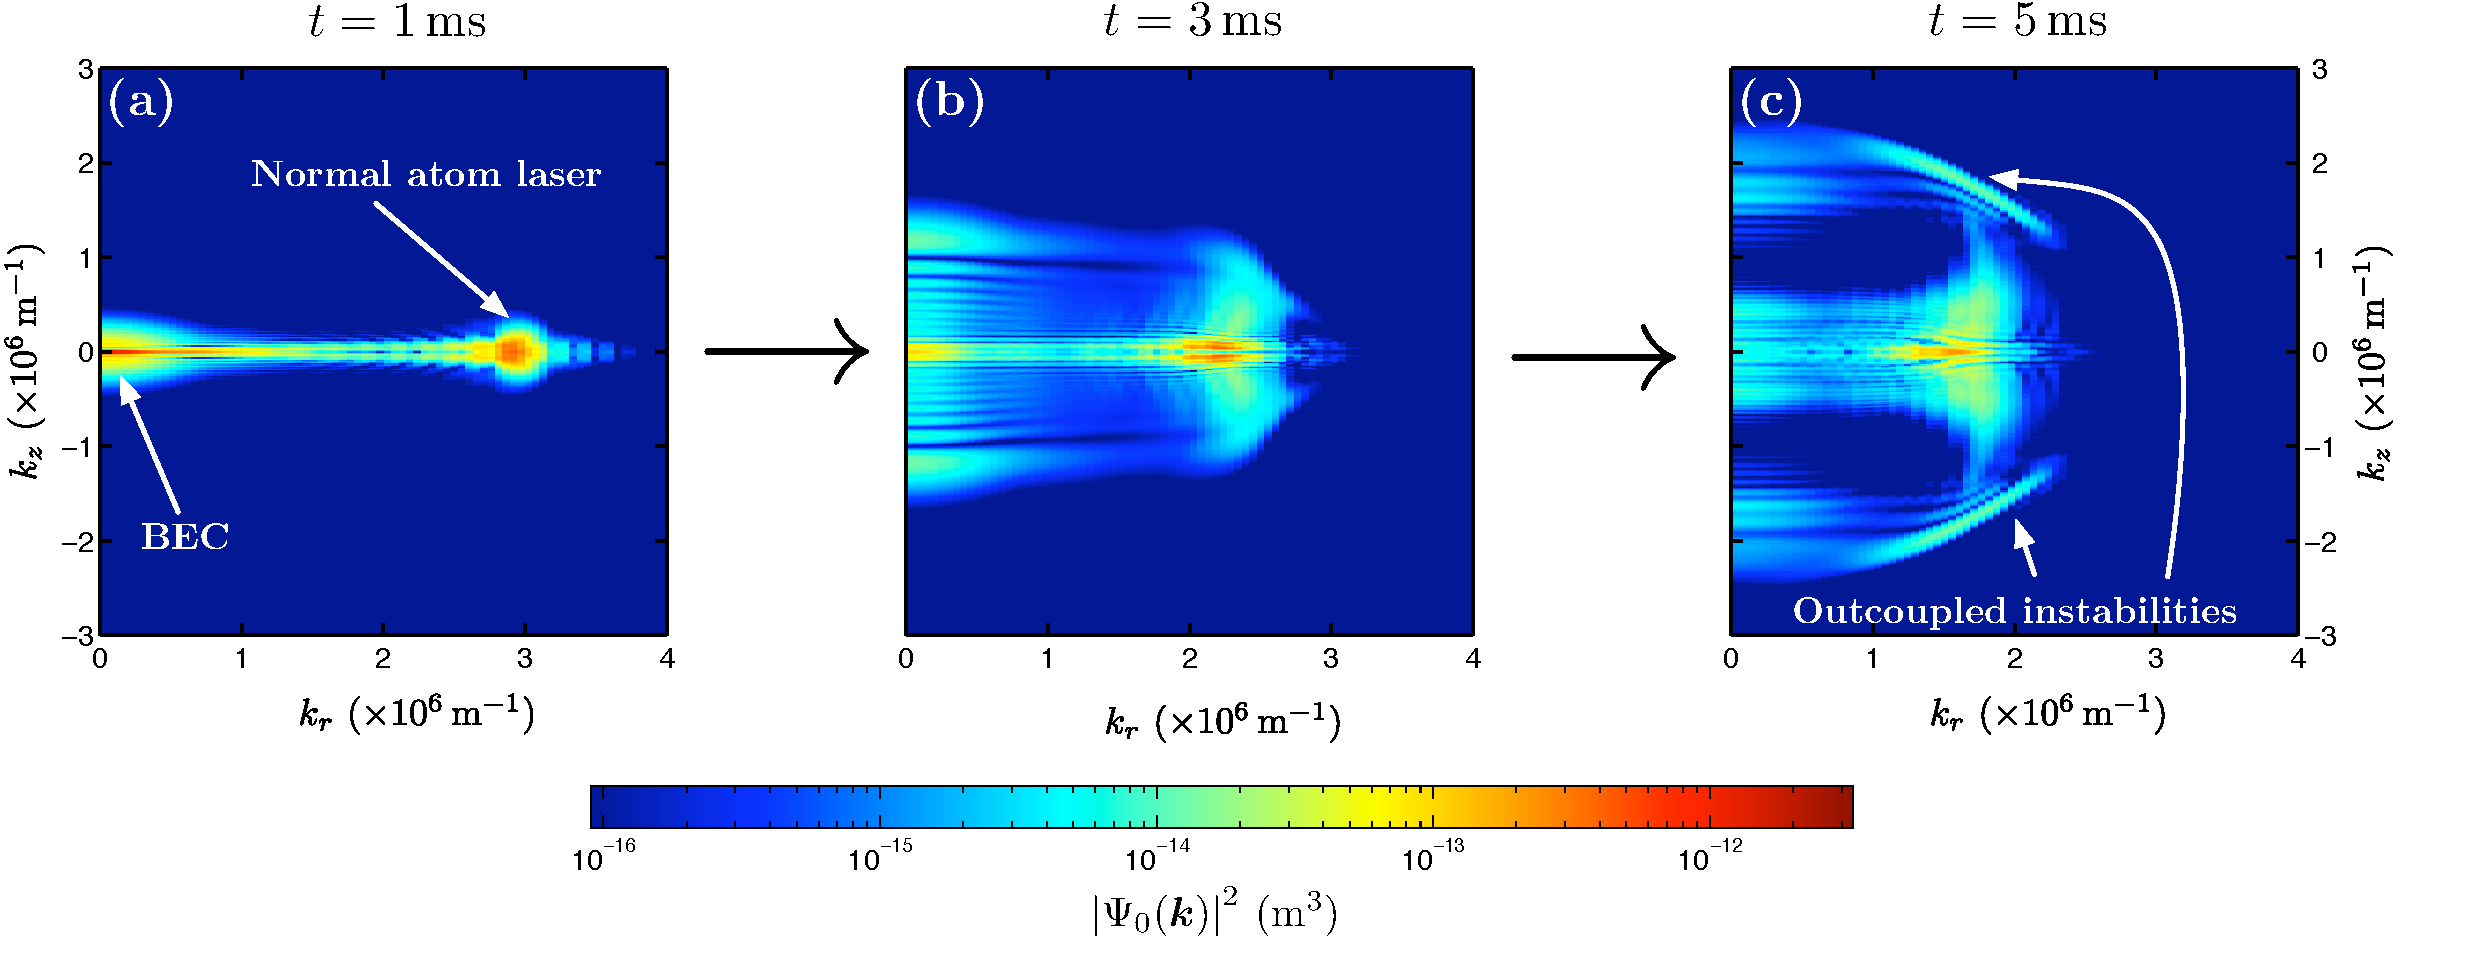
\includegraphics[width=20cm]{DetunedPeaksFormationProcess}
    \caption{Simulation results illustrating the formation of the peak-like structures due to stimulated scattering from the condensate. The results presented are from a three level GP model with a detuning of $\Delta = 2\pi \times \unit[6.5]{kHz}$ and include Penning ionisation (the results correspond to \figureref{Peaks:TheoryMaxFluxDetuningResults}(b)). Figures (a), (b), and (c) show the momentum density distribution $\abs{\Psi_0(\vect{k})}^2$ of the $m_F=0$ untrapped state at times \unit[1]{ms}, \unit[3]{ms}, and \unit[5]{ms} respectively. The marked outcoupled instabilities are the origin of the structure away from the main atom laser profile in \figureref{Peaks:ExpTheoryComparison}(e) and (f).
    \label{Peaks:DetunedPeaksFormationProcess}}
\end{sidewaysfigure}

A comparison between the experimental atom laser profile and the results of the 3-level GP simulations are presented in \figureref{Peaks:ExpTheoryComparison}.  The theoretical simulations are in excellent agreement with the experiment demonstrating that the instabilities discussed in \sectionref{Peaks:PerturbativeApproach} are the origin of the observed experimental atom laser profile.  The observed halo between the main atom laser profile and the peak-like structures at the upper and lower ends of the MCP profile are caused by the sweeping of the stimulated scattering process pictured in \figureref{Peaks:DetunedPeaksFormationProcess}.  Initially, the atom laser has negligible momentum in the weak trapping dimension ((a) of \figureref{Peaks:DetunedPeaksFormationProcess}).  This forms the central component to the atom laser profile in \figureref{Peaks:ExpTheoryComparison}(f).  As outcoupling continues the stimulated scattering process excites higher momentum modes in the axial dimension which are then outcoupled [\figureref{Peaks:DetunedPeaksFormationProcess}(b) and (c)] to form the background halo in \figureref{Peaks:ExpTheoryComparison}(f).  Once the stimulated scattering process stabilises at a maximum axial momentum, the peaks furthest from the central atom laser profile in \figureref{Peaks:ExpTheoryComparison}(f) become emphasised.

\begin{figure}
    \centering
    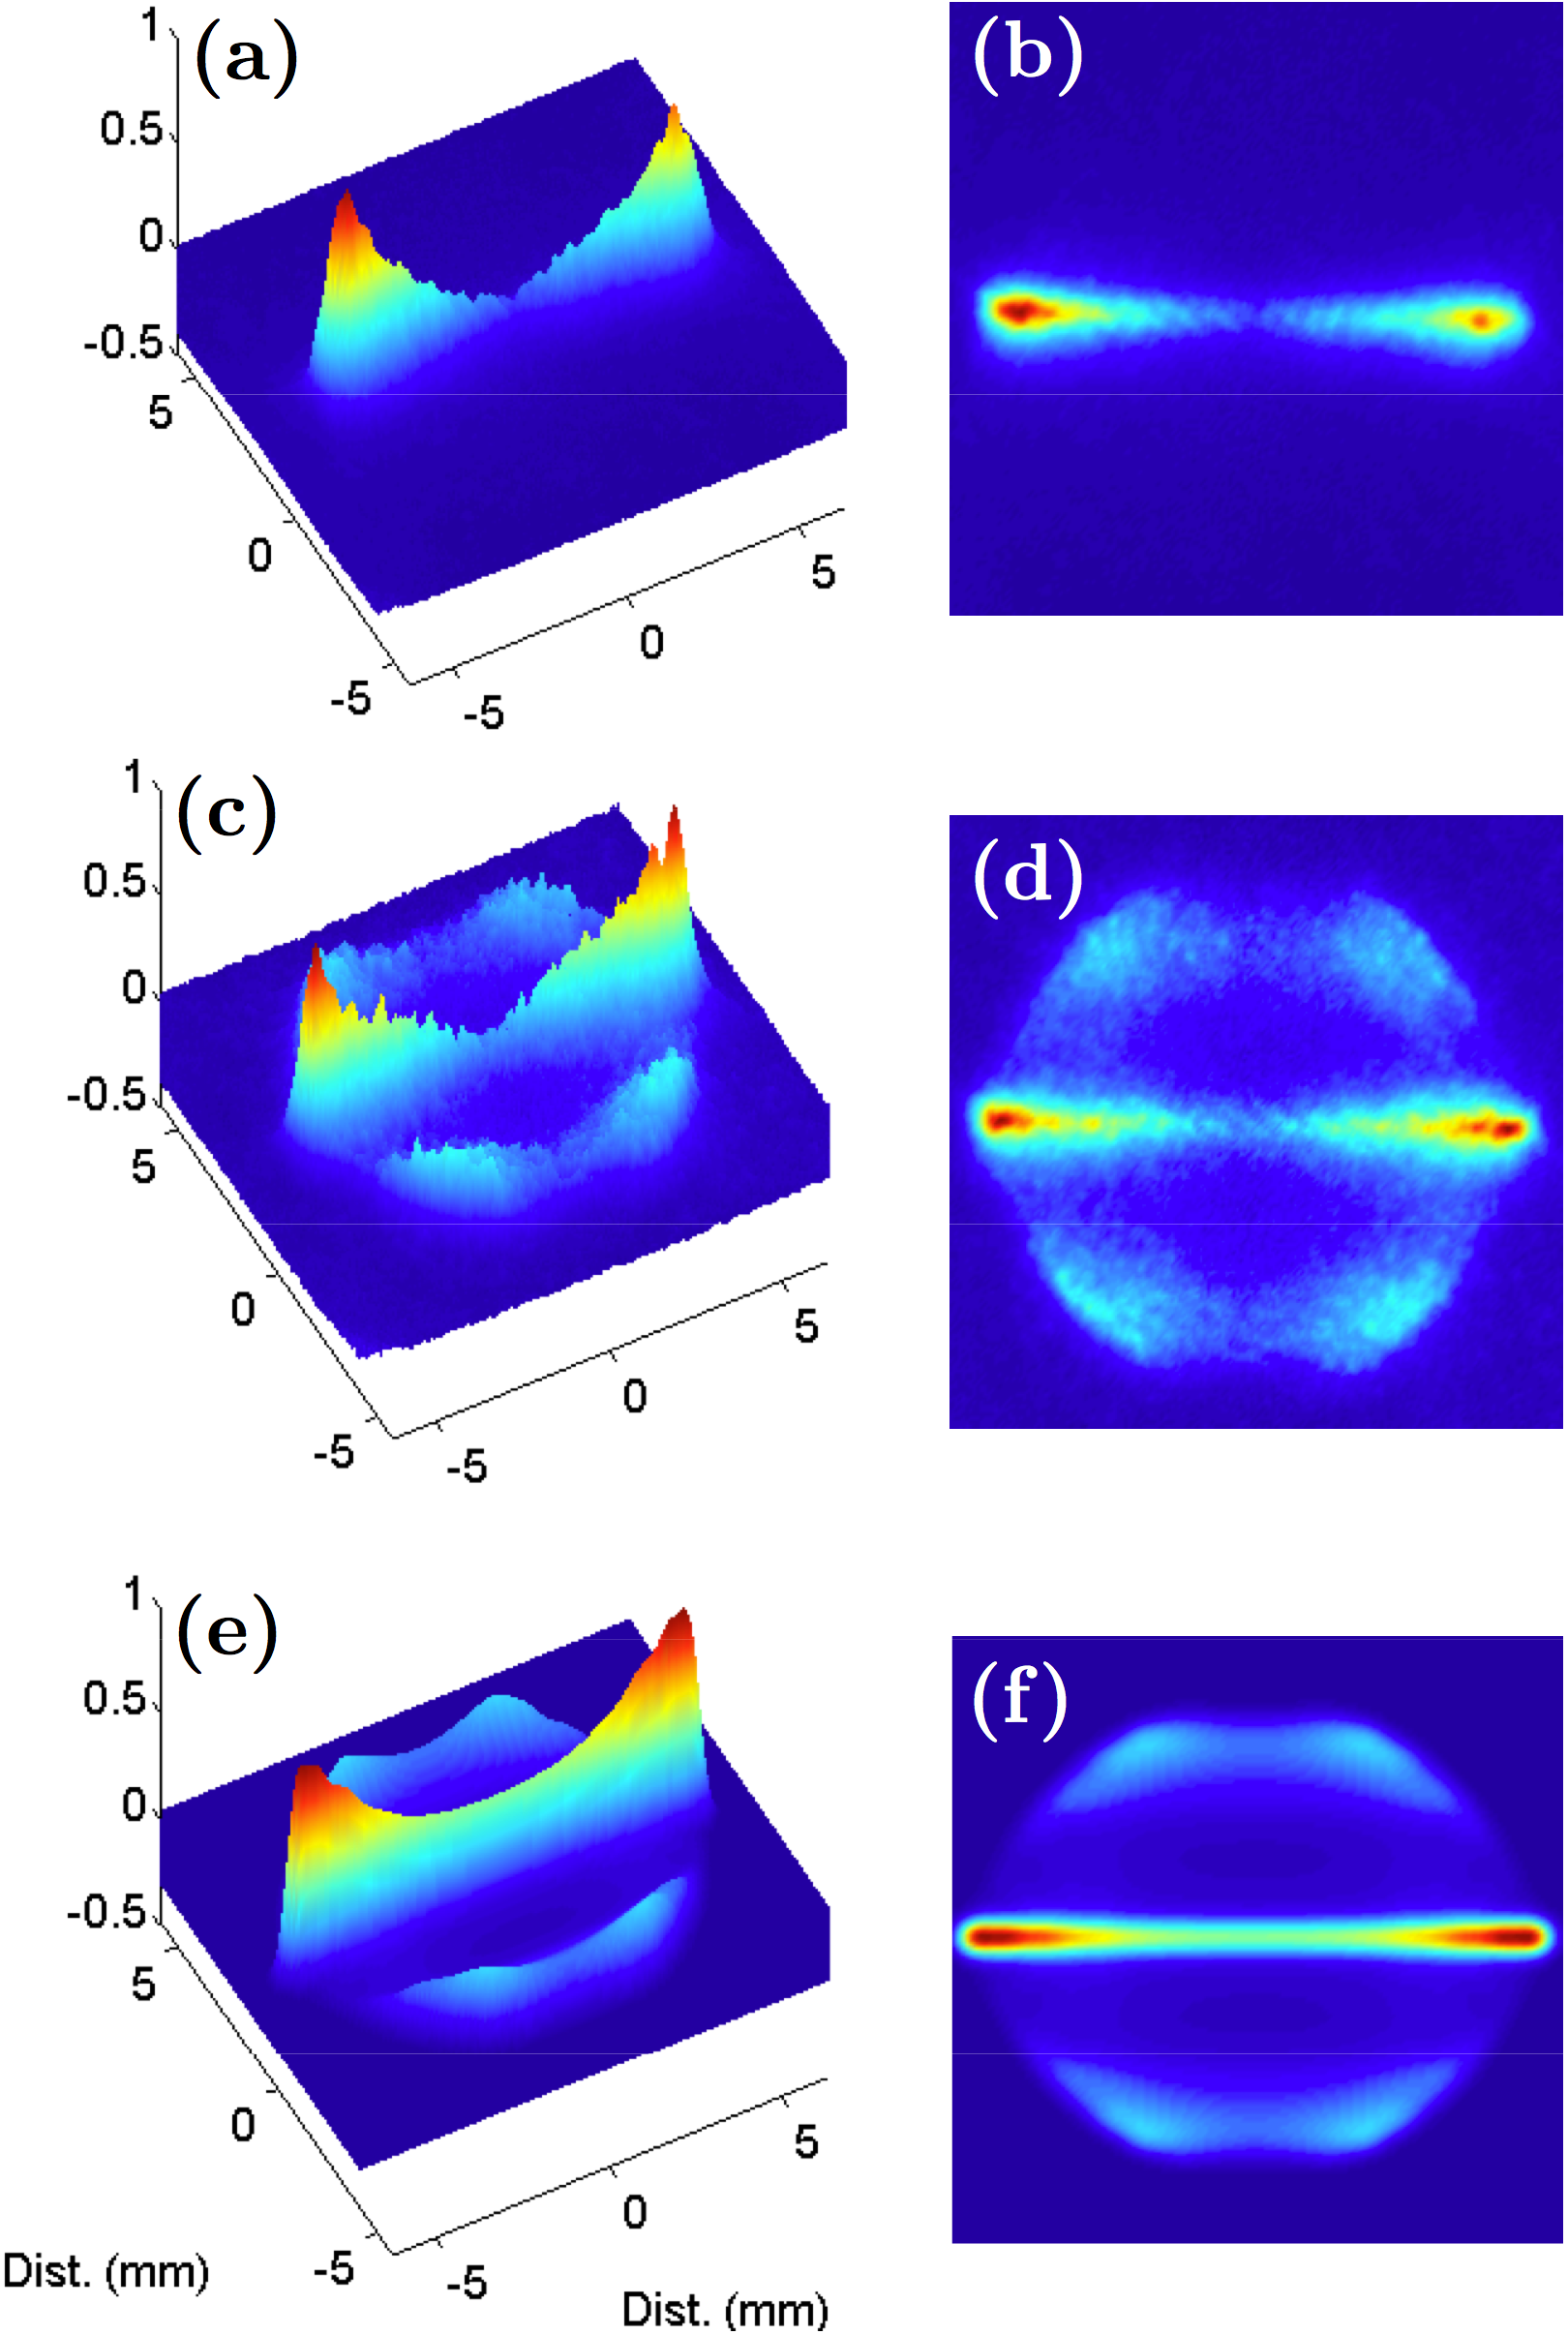
\includegraphics[width=8cm]{ExpTheoryComparison}
    \caption{First two rows show experimental atom laser spatial profiles on the MCP \unit[4]{cm} below the trap, in a three-dimensional rendering (left) and a two-dimensional image (right). Both sets of data were taken for an outcoupling detuning of \unit[6.5]{kHz}; however, the Rabi frequency is increased by an order of magnitude between the two sets. The upper row shows the usual He* atom laser (see \sectionref{BackgroundTheory:TransverseProfile}), while the middle row demonstrates the appearance of the resonant scattering peaks. The bottom row is the result of a simulation of the second experiment. The weak axis of the trap is aligned along the vertical axis of the images on the right.\label{Peaks:ExpTheoryComparison}}
\end{figure}

\subsection{Entangled beams?}

The dynamical instabilities do not need to be spontaneously seeded to be EPR-entangled.  As discussed in \sectionref{FloquetAppendix:EPREntanglement}, the optical parametric down-conversion process that drives the formation of the instabilities gives rise to EPR-entanglement even in the case that one or both of the amplified modes are initially in non-vacuum initial states.  In this case the entanglement only exists after a finite delay time.  

Although it does not follow that the outcoupled instabilities pictured in \figureref{Peaks:ExpTheoryComparison} are not entangled simply because they are predicted by the GP equation, neither can it be concluded that they are.  Certainly it cannot be checked by using a GP model, however many more simulation realisations than were used for the TW simulations presented in \figureref{Peaks:TheoryMaxFluxDetuningResults} would be necessary to verify whether or not the instabilities are entangled.  This calculation is currently infeasible as each realisation takes approximately 20 CPU-hours, and well over 1000 realisations would be necessary.  

In the case of resonant outcoupling, the excellent agreement between the results pictured in \figureref{Peaks:ResonantOutcouplingProcess} with the semianalytical model of \sectionref{Peaks:PerturbativeApproach} suggests that we can be confident that the instabilities are entangled upon formation.  The outcoupling process itself would complicate the shape of the entangled modes essentially precluding the use of this mechanism for the direct detection of entangled atomic matter waves (even if atom local oscillators in the correct states could be constructed).  That said, for both resonant and detuned outcoupling number-difference squeezing between opposite sides of the MCP detector should be robust enough to survive outcoupling.  These correlations will only exist in the time-integrated profiles as it will not be possible to determine when the other atom in the pair should arrive on the other side of the detector as the process discussed in this chapter is continuous, and hence a space-time reconstruction of the momentum distribution such as that performed in~\citep{Perrin:2007} is not possible.

Although it was not possible to investigate the existence of number-difference squeezing in the experiment described in this chapter, a recent upgrade to the experimental apparatus to include a high-resolution detector similar to that used by~\citet{Perrin:2007} has made this a possibility.  The author is hopeful that an experiment to look for the predicted number-difference squeezing will be performed in the near future.

\section{Conclusion}

In this chapter an unusual process in an atom laser was investigated.  The process involved the direct conversion of mean-field energy to the kinetic energy of unstable modes in the condensate.  This process was shown to generate entanglement in certain regimes, although in the experiment discussed it is unlikely that this entanglement remains in the outcoupled atom laser, and certainly not in any useful form.  These problems are however not fundamental.  A differently-designed experiment could overcome some of these problems to potentially produce entangled atom lasers.

One possibility worthwhile investigating would be to use a highly elongated two-state condensate in which both states experience the same trapping potential.  This could be achieved for example through the use of an optical dipole trap, or by trapping the $F=1$, $m_F=-1$ and $F=2$, $m_F=1$ \nucl{87}{Rb} states in the same magnetic trap.  As the two states of the condensate experience the same trapping potential, the two components of the dynamical instabilities would propagate together avoiding the problem of one of the components of the entangled modes leaving the condensate without the other.  Further, due to the high aspect ratio, the instabilities would propagate solely along the axial dimension.  To extract the entangled beams, one could ensure that the kinetic energy of the instabilities was higher than the trapping potential in the case of an optical dipole trap, or turn off the magnetic trap to allow the entangled beams to expand ballistically and separate from the condensate in the axial direction.  This experiment may then enable the production of highly-directional entangled atom lasers that would also be continuous in the case of the optical dipole trap.  Further theoretical investigation would be necessary to determine if such an experiment were feasible.

\parasep

\begin{quote}
    \emph{The most exciting phrase to hear in science, the one that heralds new discoveries, is not ``Eureka!'' but ``That's funny\dots''} --- Isaac Asimov
\end{quote}

The interaction between theory and experiment is a two-way street.  As a theorist, one might like to think that you can simply do some calculations, make some interesting predictions and then try to convince an experimentalist to test them.  While this is certainly a large part of the interaction, it sometimes goes the other way.  Sometimes the experimentalist tries something and the results show something that she didn't expect. ``That's funny,'' says the experimentalist.  She shows the results to the theorist and asks what might be going on.  ``That's funny,'' says the theorist\dots

This chapter is the story of one such interaction.

%This chapter has presented the results of one such interaction.  While they are not a major discovery by any stretch of the imagination, they are a testament to the accuracy of the theoretical techniques available for describing Bose-condensed systems that experimental results as strange as those presented in \figureref{Peaks:ExpTheoryComparison} can be accurately explained by theoretical calculations.


